%%
%% Template thesis.tex
%%
\documentclass{StyFiles/usydthesis}
\usepackage[palatino]{StyFiles/anuthesis}
\usepackage{StyFiles/my_macros}

%% Contents
\usepackage{makeidx}

%% Figures
\usepackage{graphicx}
\usepackage{hyperref}

%% Features
\usepackage{StyFiles/fancyhdr}
\usepackage{url}
\usepackage{makecell}
\usepackage{textcomp}
\usepackage{booktabs}
\usepackage{multirow}
\usepackage[normalem]{ulem}
\useunder{\uline}{\ul}{}

%% Formats
\usepackage[toc,page]{appendix}
\usepackage[font=small,labelfont=bf]{caption}
\usepackage[font=footnotesize]{subfig}
\usepackage{StyFiles/hyphenat}
% correct bad hyphenation here
\hyphenation{op-tical net-works semi-conduc-tor}

%% Algos
\usepackage{StyFiles/algorithm}
\usepackage{StyFiles/algorithmic}
\usepackage[algo2e,ruled,vlined,linesnumbered]{algorithm2e}
\newcommand{\fix}{\marginpar{FIX}}
\newcommand{\new}{\marginpar{NEW}}


%% For maths
\usepackage[cmex10]{amsmath}
\usepackage{amssymb,amsthm}
%%%%% NEW MATH DEFINITIONS %%%%%

\usepackage{amsmath,amsfonts,bm}

% Mark sections of captions for referring to divisions of figures
\newcommand{\figleft}{{\em (Left)}}
\newcommand{\figcenter}{{\em (Center)}}
\newcommand{\figright}{{\em (Right)}}
\newcommand{\figtop}{{\em (Top)}}
\newcommand{\figbottom}{{\em (Bottom)}}
\newcommand{\captiona}{{\em (a)}}
\newcommand{\captionb}{{\em (b)}}
\newcommand{\captionc}{{\em (c)}}
\newcommand{\captiond}{{\em (d)}}

% Highlight a newly defined term
\newcommand{\newterm}[1]{{\bf #1}}


% Figure reference, lower-case.
\def\figref#1{figure~\ref{#1}}
% Figure reference, capital. For start of sentence
\def\Figref#1{Figure~\ref{#1}}
\def\twofigref#1#2{figures \ref{#1} and \ref{#2}}
\def\quadfigref#1#2#3#4{figures \ref{#1}, \ref{#2}, \ref{#3} and \ref{#4}}
% Section reference, lower-case.
\def\secref#1{section~\ref{#1}}
% Section reference, capital.
\def\Secref#1{Section~\ref{#1}}
% Reference to two sections.
\def\twosecrefs#1#2{sections \ref{#1} and \ref{#2}}
% Reference to three sections.
\def\secrefs#1#2#3{sections \ref{#1}, \ref{#2} and \ref{#3}}
% Reference to an equation, lower-case.
\def\eqref#1{equation~\ref{#1}}
% Reference to an equation, upper case
\def\Eqref#1{Equation~\ref{#1}}
% A raw reference to an equation---avoid using if possible
\def\plaineqref#1{\ref{#1}}
% Reference to a chapter, lower-case.
\def\chapref#1{chapter~\ref{#1}}
% Reference to an equation, upper case.
\def\Chapref#1{Chapter~\ref{#1}}
% Reference to a range of chapters
\def\rangechapref#1#2{chapters\ref{#1}--\ref{#2}}
% Reference to an algorithm, lower-case.
\def\algref#1{algorithm~\ref{#1}}
% Reference to an algorithm, upper case.
\def\Algref#1{Algorithm~\ref{#1}}
\def\twoalgref#1#2{algorithms \ref{#1} and \ref{#2}}
\def\Twoalgref#1#2{Algorithms \ref{#1} and \ref{#2}}
% Reference to a part, lower case
\def\partref#1{part~\ref{#1}}
% Reference to a part, upper case
\def\Partref#1{Part~\ref{#1}}
\def\twopartref#1#2{parts \ref{#1} and \ref{#2}}

\def\ceil#1{\lceil #1 \rceil}
\def\floor#1{\lfloor #1 \rfloor}
\def\1{\bm{1}}
\newcommand{\train}{\mathcal{D}}
\newcommand{\valid}{\mathcal{D_{\mathrm{valid}}}}
\newcommand{\test}{\mathcal{D_{\mathrm{test}}}}

\def\eps{{\epsilon}}


% Random variables
\def\reta{{\textnormal{$\eta$}}}
\def\ra{{\textnormal{a}}}
\def\rb{{\textnormal{b}}}
\def\rc{{\textnormal{c}}}
\def\rd{{\textnormal{d}}}
\def\re{{\textnormal{e}}}
\def\rf{{\textnormal{f}}}
\def\rg{{\textnormal{g}}}
\def\rh{{\textnormal{h}}}
\def\ri{{\textnormal{i}}}
\def\rj{{\textnormal{j}}}
\def\rk{{\textnormal{k}}}
\def\rl{{\textnormal{l}}}
% rm is already a command, just don't name any random variables m
\def\rn{{\textnormal{n}}}
\def\ro{{\textnormal{o}}}
\def\rp{{\textnormal{p}}}
\def\rq{{\textnormal{q}}}
\def\rr{{\textnormal{r}}}
\def\rs{{\textnormal{s}}}
\def\rt{{\textnormal{t}}}
\def\ru{{\textnormal{u}}}
\def\rv{{\textnormal{v}}}
\def\rw{{\textnormal{w}}}
\def\rx{{\textnormal{x}}}
\def\ry{{\textnormal{y}}}
\def\rz{{\textnormal{z}}}

% Random vectors
\def\rvepsilon{{\mathbf{\epsilon}}}
\def\rvtheta{{\mathbf{\theta}}}
\def\rva{{\mathbf{a}}}
\def\rvb{{\mathbf{b}}}
\def\rvc{{\mathbf{c}}}
\def\rvd{{\mathbf{d}}}
\def\rve{{\mathbf{e}}}
\def\rvf{{\mathbf{f}}}
\def\rvg{{\mathbf{g}}}
\def\rvh{{\mathbf{h}}}
\def\rvu{{\mathbf{i}}}
\def\rvj{{\mathbf{j}}}
\def\rvk{{\mathbf{k}}}
\def\rvl{{\mathbf{l}}}
\def\rvm{{\mathbf{m}}}
\def\rvn{{\mathbf{n}}}
\def\rvo{{\mathbf{o}}}
\def\rvp{{\mathbf{p}}}
\def\rvq{{\mathbf{q}}}
\def\rvr{{\mathbf{r}}}
\def\rvs{{\mathbf{s}}}
\def\rvt{{\mathbf{t}}}
\def\rvu{{\mathbf{u}}}
\def\rvv{{\mathbf{v}}}
\def\rvw{{\mathbf{w}}}
\def\rvx{{\mathbf{x}}}
\def\rvy{{\mathbf{y}}}
\def\rvz{{\mathbf{z}}}

% Elements of random vectors
\def\erva{{\textnormal{a}}}
\def\ervb{{\textnormal{b}}}
\def\ervc{{\textnormal{c}}}
\def\ervd{{\textnormal{d}}}
\def\erve{{\textnormal{e}}}
\def\ervf{{\textnormal{f}}}
\def\ervg{{\textnormal{g}}}
\def\ervh{{\textnormal{h}}}
\def\ervi{{\textnormal{i}}}
\def\ervj{{\textnormal{j}}}
\def\ervk{{\textnormal{k}}}
\def\ervl{{\textnormal{l}}}
\def\ervm{{\textnormal{m}}}
\def\ervn{{\textnormal{n}}}
\def\ervo{{\textnormal{o}}}
\def\ervp{{\textnormal{p}}}
\def\ervq{{\textnormal{q}}}
\def\ervr{{\textnormal{r}}}
\def\ervs{{\textnormal{s}}}
\def\ervt{{\textnormal{t}}}
\def\ervu{{\textnormal{u}}}
\def\ervv{{\textnormal{v}}}
\def\ervw{{\textnormal{w}}}
\def\ervx{{\textnormal{x}}}
\def\ervy{{\textnormal{y}}}
\def\ervz{{\textnormal{z}}}

% Random matrices
\def\rmA{{\mathbf{A}}}
\def\rmB{{\mathbf{B}}}
\def\rmC{{\mathbf{C}}}
\def\rmD{{\mathbf{D}}}
\def\rmE{{\mathbf{E}}}
\def\rmF{{\mathbf{F}}}
\def\rmG{{\mathbf{G}}}
\def\rmH{{\mathbf{H}}}
\def\rmI{{\mathbf{I}}}
\def\rmJ{{\mathbf{J}}}
\def\rmK{{\mathbf{K}}}
\def\rmL{{\mathbf{L}}}
\def\rmM{{\mathbf{M}}}
\def\rmN{{\mathbf{N}}}
\def\rmO{{\mathbf{O}}}
\def\rmP{{\mathbf{P}}}
\def\rmQ{{\mathbf{Q}}}
\def\rmR{{\mathbf{R}}}
\def\rmS{{\mathbf{S}}}
\def\rmT{{\mathbf{T}}}
\def\rmU{{\mathbf{U}}}
\def\rmV{{\mathbf{V}}}
\def\rmW{{\mathbf{W}}}
\def\rmX{{\mathbf{X}}}
\def\rmY{{\mathbf{Y}}}
\def\rmZ{{\mathbf{Z}}}

% Elements of random matrices
\def\ermA{{\textnormal{A}}}
\def\ermB{{\textnormal{B}}}
\def\ermC{{\textnormal{C}}}
\def\ermD{{\textnormal{D}}}
\def\ermE{{\textnormal{E}}}
\def\ermF{{\textnormal{F}}}
\def\ermG{{\textnormal{G}}}
\def\ermH{{\textnormal{H}}}
\def\ermI{{\textnormal{I}}}
\def\ermJ{{\textnormal{J}}}
\def\ermK{{\textnormal{K}}}
\def\ermL{{\textnormal{L}}}
\def\ermM{{\textnormal{M}}}
\def\ermN{{\textnormal{N}}}
\def\ermO{{\textnormal{O}}}
\def\ermP{{\textnormal{P}}}
\def\ermQ{{\textnormal{Q}}}
\def\ermR{{\textnormal{R}}}
\def\ermS{{\textnormal{S}}}
\def\ermT{{\textnormal{T}}}
\def\ermU{{\textnormal{U}}}
\def\ermV{{\textnormal{V}}}
\def\ermW{{\textnormal{W}}}
\def\ermX{{\textnormal{X}}}
\def\ermY{{\textnormal{Y}}}
\def\ermZ{{\textnormal{Z}}}

% Vectors
\def\vzero{{\bm{0}}}
\def\vone{{\bm{1}}}
\def\vmu{{\bm{\mu}}}
\def\vtheta{{\bm{\theta}}}
\def\va{{\bm{a}}}
\def\vb{{\bm{b}}}
\def\vc{{\bm{c}}}
\def\vd{{\bm{d}}}
\def\ve{{\bm{e}}}
\def\vf{{\bm{f}}}
\def\vg{{\bm{g}}}
\def\vh{{\bm{h}}}
\def\vi{{\bm{i}}}
\def\vj{{\bm{j}}}
\def\vk{{\bm{k}}}
\def\vl{{\bm{l}}}
\def\vm{{\bm{m}}}
\def\vn{{\bm{n}}}
\def\vo{{\bm{o}}}
\def\vp{{\bm{p}}}
\def\vq{{\bm{q}}}
\def\vr{{\bm{r}}}
\def\vs{{\bm{s}}}
\def\vt{{\bm{t}}}
\def\vu{{\bm{u}}}
\def\vv{{\bm{v}}}
\def\vw{{\bm{w}}}
\def\vx{{\bm{x}}}
\def\vy{{\bm{y}}}
\def\vz{{\bm{z}}}

% Elements of vectors
\def\evalpha{{\alpha}}
\def\evbeta{{\beta}}
\def\evepsilon{{\epsilon}}
\def\evlambda{{\lambda}}
\def\evomega{{\omega}}
\def\evmu{{\mu}}
\def\evpsi{{\psi}}
\def\evsigma{{\sigma}}
\def\evtheta{{\theta}}
\def\eva{{a}}
\def\evb{{b}}
\def\evc{{c}}
\def\evd{{d}}
\def\eve{{e}}
\def\evf{{f}}
\def\evg{{g}}
\def\evh{{h}}
\def\evi{{i}}
\def\evj{{j}}
\def\evk{{k}}
\def\evl{{l}}
\def\evm{{m}}
\def\evn{{n}}
\def\evo{{o}}
\def\evp{{p}}
\def\evq{{q}}
\def\evr{{r}}
\def\evs{{s}}
\def\evt{{t}}
\def\evu{{u}}
\def\evv{{v}}
\def\evw{{w}}
\def\evx{{x}}
\def\evy{{y}}
\def\evz{{z}}

% Matrix
\def\mA{{\bm{A}}}
\def\mB{{\bm{B}}}
\def\mC{{\bm{C}}}
\def\mD{{\bm{D}}}
\def\mE{{\bm{E}}}
\def\mF{{\bm{F}}}
\def\mG{{\bm{G}}}
\def\mH{{\bm{H}}}
\def\mI{{\bm{I}}}
\def\mJ{{\bm{J}}}
\def\mK{{\bm{K}}}
\def\mL{{\bm{L}}}
\def\mM{{\bm{M}}}
\def\mN{{\bm{N}}}
\def\mO{{\bm{O}}}
\def\mP{{\bm{P}}}
\def\mQ{{\bm{Q}}}
\def\mR{{\bm{R}}}
\def\mS{{\bm{S}}}
\def\mT{{\bm{T}}}
\def\mU{{\bm{U}}}
\def\mV{{\bm{V}}}
\def\mW{{\bm{W}}}
\def\mX{{\bm{X}}}
\def\mY{{\bm{Y}}}
\def\mZ{{\bm{Z}}}
\def\mBeta{{\bm{\beta}}}
\def\mPhi{{\bm{\Phi}}}
\def\mLambda{{\bm{\Lambda}}}
\def\mSigma{{\bm{\Sigma}}}

% Tensor
\DeclareMathAlphabet{\mathsfit}{\encodingdefault}{\sfdefault}{m}{sl}
\SetMathAlphabet{\mathsfit}{bold}{\encodingdefault}{\sfdefault}{bx}{n}
\newcommand{\tens}[1]{\bm{\mathsfit{#1}}}
\def\tA{{\tens{A}}}
\def\tB{{\tens{B}}}
\def\tC{{\tens{C}}}
\def\tD{{\tens{D}}}
\def\tE{{\tens{E}}}
\def\tF{{\tens{F}}}
\def\tG{{\tens{G}}}
\def\tH{{\tens{H}}}
\def\tI{{\tens{I}}}
\def\tJ{{\tens{J}}}
\def\tK{{\tens{K}}}
\def\tL{{\tens{L}}}
\def\tM{{\tens{M}}}
\def\tN{{\tens{N}}}
\def\tO{{\tens{O}}}
\def\tP{{\tens{P}}}
\def\tQ{{\tens{Q}}}
\def\tR{{\tens{R}}}
\def\tS{{\tens{S}}}
\def\tT{{\tens{T}}}
\def\tU{{\tens{U}}}
\def\tV{{\tens{V}}}
\def\tW{{\tens{W}}}
\def\tX{{\tens{X}}}
\def\tY{{\tens{Y}}}
\def\tZ{{\tens{Z}}}


% Graph
\def\gA{{\mathcal{A}}}
\def\gB{{\mathcal{B}}}
\def\gC{{\mathcal{C}}}
\def\gD{{\mathcal{D}}}
\def\gE{{\mathcal{E}}}
\def\gF{{\mathcal{F}}}
\def\gG{{\mathcal{G}}}
\def\gH{{\mathcal{H}}}
\def\gI{{\mathcal{I}}}
\def\gJ{{\mathcal{J}}}
\def\gK{{\mathcal{K}}}
\def\gL{{\mathcal{L}}}
\def\gM{{\mathcal{M}}}
\def\gN{{\mathcal{N}}}
\def\gO{{\mathcal{O}}}
\def\gP{{\mathcal{P}}}
\def\gQ{{\mathcal{Q}}}
\def\gR{{\mathcal{R}}}
\def\gS{{\mathcal{S}}}
\def\gT{{\mathcal{T}}}
\def\gU{{\mathcal{U}}}
\def\gV{{\mathcal{V}}}
\def\gW{{\mathcal{W}}}
\def\gX{{\mathcal{X}}}
\def\gY{{\mathcal{Y}}}
\def\gZ{{\mathcal{Z}}}

% Sets
\def\sA{{\mathbb{A}}}
\def\sB{{\mathbb{B}}}
\def\sC{{\mathbb{C}}}
\def\sD{{\mathbb{D}}}
% Don't use a set called E, because this would be the same as our symbol
% for expectation.
\def\sF{{\mathbb{F}}}
\def\sG{{\mathbb{G}}}
\def\sH{{\mathbb{H}}}
\def\sI{{\mathbb{I}}}
\def\sJ{{\mathbb{J}}}
\def\sK{{\mathbb{K}}}
\def\sL{{\mathbb{L}}}
\def\sM{{\mathbb{M}}}
\def\sN{{\mathbb{N}}}
\def\sO{{\mathbb{O}}}
\def\sP{{\mathbb{P}}}
\def\sQ{{\mathbb{Q}}}
\def\sR{{\mathbb{R}}}
\def\sS{{\mathbb{S}}}
\def\sT{{\mathbb{T}}}
\def\sU{{\mathbb{U}}}
\def\sV{{\mathbb{V}}}
\def\sW{{\mathbb{W}}}
\def\sX{{\mathbb{X}}}
\def\sY{{\mathbb{Y}}}
\def\sZ{{\mathbb{Z}}}

% Entries of a matrix
\def\emLambda{{\Lambda}}
\def\emA{{A}}
\def\emB{{B}}
\def\emC{{C}}
\def\emD{{D}}
\def\emE{{E}}
\def\emF{{F}}
\def\emG{{G}}
\def\emH{{H}}
\def\emI{{I}}
\def\emJ{{J}}
\def\emK{{K}}
\def\emL{{L}}
\def\emM{{M}}
\def\emN{{N}}
\def\emO{{O}}
\def\emP{{P}}
\def\emQ{{Q}}
\def\emR{{R}}
\def\emS{{S}}
\def\emT{{T}}
\def\emU{{U}}
\def\emV{{V}}
\def\emW{{W}}
\def\emX{{X}}
\def\emY{{Y}}
\def\emZ{{Z}}
\def\emSigma{{\Sigma}}

% entries of a tensor
% Same font as tensor, without \bm wrapper
\newcommand{\etens}[1]{\mathsfit{#1}}
\def\etLambda{{\etens{\Lambda}}}
\def\etA{{\etens{A}}}
\def\etB{{\etens{B}}}
\def\etC{{\etens{C}}}
\def\etD{{\etens{D}}}
\def\etE{{\etens{E}}}
\def\etF{{\etens{F}}}
\def\etG{{\etens{G}}}
\def\etH{{\etens{H}}}
\def\etI{{\etens{I}}}
\def\etJ{{\etens{J}}}
\def\etK{{\etens{K}}}
\def\etL{{\etens{L}}}
\def\etM{{\etens{M}}}
\def\etN{{\etens{N}}}
\def\etO{{\etens{O}}}
\def\etP{{\etens{P}}}
\def\etQ{{\etens{Q}}}
\def\etR{{\etens{R}}}
\def\etS{{\etens{S}}}
\def\etT{{\etens{T}}}
\def\etU{{\etens{U}}}
\def\etV{{\etens{V}}}
\def\etW{{\etens{W}}}
\def\etX{{\etens{X}}}
\def\etY{{\etens{Y}}}
\def\etZ{{\etens{Z}}}

% The true underlying data generating distribution
\newcommand{\pdata}{p_{\rm{data}}}
% The empirical distribution defined by the training set
\newcommand{\ptrain}{\hat{p}_{\rm{data}}}
\newcommand{\Ptrain}{\hat{P}_{\rm{data}}}
% The model distribution
\newcommand{\pmodel}{p_{\rm{model}}}
\newcommand{\Pmodel}{P_{\rm{model}}}
\newcommand{\ptildemodel}{\tilde{p}_{\rm{model}}}
% Stochastic autoencoder distributions
\newcommand{\pencode}{p_{\rm{encoder}}}
\newcommand{\pdecode}{p_{\rm{decoder}}}
\newcommand{\precons}{p_{\rm{reconstruct}}}

\newcommand{\laplace}{\mathrm{Laplace}} % Laplace distribution

\newcommand{\E}{\mathbb{E}}
\newcommand{\Ls}{\mathcal{L}}
\newcommand{\R}{\mathbb{R}}
\newcommand{\emp}{\tilde{p}}
\newcommand{\lr}{\alpha}
\newcommand{\reg}{\lambda}
\newcommand{\rect}{\mathrm{rectifier}}
\newcommand{\softmax}{\mathrm{softmax}}
\newcommand{\sigmoid}{\sigma}
\newcommand{\softplus}{\zeta}
\newcommand{\KL}{D_{\mathrm{KL}}}
\newcommand{\Var}{\mathrm{Var}}
\newcommand{\standarderror}{\mathrm{SE}}
\newcommand{\Cov}{\mathrm{Cov}}
% Wolfram Mathworld says $L^2$ is for function spaces and $\ell^2$ is for vectors
% But then they seem to use $L^2$ for vectors throughout the site, and so does
% wikipedia.
\newcommand{\normlzero}{L^0}
\newcommand{\normlone}{L^1}
\newcommand{\normltwo}{L^2}
\newcommand{\normlp}{L^p}
\newcommand{\normmax}{L^\infty}

\newcommand{\parents}{Pa} % See usage in notation.tex. Chosen to match Daphne's book.

\DeclareMathOperator*{\argmax}{arg\,max}
\DeclareMathOperator*{\argmin}{arg\,min}

\DeclareMathOperator{\sign}{sign}
\DeclareMathOperator{\Tr}{Tr}
\let\ab\allowbreak


%% Commands
\newcommand{\mmqp}[3]{\textrm{\sc MaxMarginQP}\!\left(\{\by_t, #1\}_{t=1}^{T}, #2, #3\right)}
\newcommand{\energy}[1]{\ensuremath{E\!\left(#1\right)}}
\newcommand{\bigCI}{\mathrel{\text{\scalebox{1.07}{$\perp\mkern-10mu\perp$}}}}

%% Environments
\newtheorem{thm}{Theorem}[section]
\newtheorem{cor}[thm]{Corollary}
\newtheorem{lem}[thm]{Lemma}
\newtheorem{prop}[thm]{Proposition}
\newtheorem{obs}[thm]{Observation}
\newtheorem{defn}[thm]{Definition}

%%%%%%%%%%%%%%%%%%%%%%%%%%%%%%%%%%%%%%%%%%%%%%%%%%%%%%%%%%%%%%%%%%%%%%%
%% Preamble
\renewcommand{\thepage}{\roman{page}}

\makeindex
\begin{document}

\singlespacing
\pagenumbering{roman}  % first use Roman numerals for page numbers
% initial page numbers:  i, ii, iii, ...
\renewcommand{\thepage}{\roman{page}}	
%%%%%%%%%%%%
% Title page
\font\myfont=cmr12 at 20pt 
\title{{\myfont\bf SEQUENCE LEARNING USING DEEP NEURAL NETWORKS WITH FLEXIBILITY AND INTERPRETABILITY}}
\author{Chang Li}
\def\thisauthor{Chang Li}
\def\degree{Doctor of Philosophy}
\def\department{School of Computer Science \\ Faculty of Engineering}
\def\mydegrees{Doctor of Philosophy (Ph.D.)}
\def\supervisor{Dacheng Tao}
\def\assocsupervisora{Dongjin Song}
%\def\sid{200342291}
% \maketitle

\onehalfspacing
% %%%%%%%%%%%%%%%%%%%%%%%%%%%%%%%%%%%%%%%%%%%%%%%%%%%%%%%%%%%%%%%%%%%%%%%
% %% Here begin the preliminaries
% %%
%% Template frontmatter.tex (Copyright etc.)
%%

\vspace*{14cm}
\begin{center}
  \makeatletter
  \copyright\ \@author
  \makeatother
\end{center}
\noindent
\begin{center}
  \aboutthesis
\end{center}
\noindent

\newpage

\vspace*{7cm}
\begin{center}
  I certify that the intellectual content of this thesis is the
  product of my own work and that all the assistance received in
  preparing this thesis and sources have been acknowledged.
\end{center}

\vspace*{4cm}

\hspace{8cm}\makeatletter\@author\makeatother\par
\hspace{8cm}\today


%%% Local Variables: 
%%% mode: latex
%%% TeX-master: "thesis"
%%% End: 


% %%%%%%%%%%%%%%%%%%%%%%%%%%%%%%%%%%%%%%%%%%%%%%%%%%%%%%%%%%%%%%%%%%%%%%%
% %% Dedication (optional)
% \cleardoublepage
% \pagestyle{empty}
% %%
%% Template dedication.tex
%%

\vspace*{7cm}
\begin{center}
  To a world with love and equality.
\end{center}


%%% Local Variables: 
%%% mode: latex
%%% TeX-master: "thesis"
%%% End: 



% %%%%%%%%%%%%%%%%%%%%%%%%%%%%%%%%%%%%%%%%%%%%%%%%%%%%%%%%%%%%%%%%%%%%%%%
% %% Acknowledgements (optional!)
% \cleardoublepage
% \pagestyle{empty}
% %%
%% Template ack.tex
%%

\section*{\hfil Acknowledgements \hfil}

Thank you to my supervisor Dacheng Tao for his invaluable and
unconditional supports for my research during all these years.
His great patience and willingness to give his time so generously
are very much appreciated. Thank you to my associate supervisor
Dongjin Song for keep motivating and encouraging me to explore
hard challenges. The Skill-Action architecture will not be
discovered without their supports. Thank you to Shangtong Zhang
for his great open source project. Thank you to Pierre-Luc Bacon,
Matthew D Riemer and Shangtong Zhang's patience in answering my
questions. I would also like to express my very great
appreciation to the open source community (Python, OpenCV and
Chun-Nam Yu etc.). I cannot finish this work without their
generous contributions.


%%% Local Variables:
%%% mode: latex
%%% TeX-master: "../thesis"
%%% End:


% %%%%%%%%%%%%%%%%%%%%%%%%%%%%%%%%%%%%%%%%%%%%%%%%%%%%%%%%%%%%%%%%%%%%%%%
% %% Abstract
% \cleardoublepage
% \pagestyle{headings}
% %%
%% Template abstract.tex
%%

\chapter*{Abstract}
\label{cha:abstract}
\addcontentsline{toc}{chapter}{Abstract}

Throughout this thesis, I investigate two long-standing yet
rarely explored sequence learning challenges under the
Probabilistic Graphical Models (PGMs) framework: learning
multi-timescale representations on a single sequence and learning
higher-order dynamics between multi-sequences. The first
challenge is tackled with Hidden Markov Models (HMMs), a type of
directed PGMs, under the reinforcement learning framework. With
the help of conditional independence properties encoded in HMMs,
I prove that the Semi-Markov Decision Problem (SMDP) formulated
option framework
\cite{sutton1999between,bacon2017option,zhang2019dac}, one of the
most promising Hierarchical Reinforcement Learning (HRL)
frameworks, has a Markov Decision Problem (MDP) equivalence.
Based on this equivalence, a simple yet effective Skill-Action
(SA) architecture is proposed. SA can not only extract skills
(abstract actions) hierarchically from primary actions into skill
context vectors (embedding vectors), but also temporally extend
skills by employing the attention mechanism. Our empirical
studies on challenging robot simulation environments demonstrate
that SA significantly outperforms all baselines on both
single-task infinite horizon environments and transfer learning
environments. Compared to other option variants, SA has smaller
variance, faster convergence, and better interpretability.
Because of its exceptional scalability, SA has the potential to
pave the way for a large scale pre-training architecture in
reinforcement learning.

The second challenge is tackled with Markov Random Fields (MRFs),
also known as undirected PGMs, under the supervised learning
framework. I employ binary MRFs with weighted Lower Linear
Envelope Potentials (LLEPs) as the higher-order energy function
to capture higher-order dependencies. I propose an exact
inference algorithm under the graph-cuts framework and an
efficient learning algorithm under the Latent Structural Support
Vector Machines (LSSVMs) framework. Experiments on synthetic
checkerboard show that the novel formulation of binary MRFs can
learn LLEPs exactly other than previous studies which can only
learn LLEPs approximately
\cite{gouldlearning,narayanaswamy2017learning}. I extend this
model to learn higher-order dynamics between time series and
conduct experiments on financial stock data set. Stock price's
movements not only depend on the historical price of an
individual stock, but also has unobserved higher order dynamics
with other correlated stocks. In order to learn these
higher-order latent dynamics, we present a multi-task recurrent
neural network (RNN) with high-order Markov random fields (MRFs)
to predict directions of stock price movements. Specifically, I
first design a multi-task RNN framework to extract informative
features from the raw market data of individual stocks without
considering any domain knowledge. Then a sub-gradient algorithm
is employed to perform end-to-end training of the RNN and the
binary MRFs with high-order energy functions. We conduct thorough
empirical studies on three popular Chinese stock market indexes
and the proposed method outperforms baseline approaches. To our
best knowledge, the proposed technique is the first to
investigate intra-clique relationships with higher-order MRFs for
stock price movement prediction.

%%% Local Variables: 
%%% mode: latex
%%% TeX-master: "thesis"
%%% End: 


%%%%%%%%%%%%%%%%%%%%%%%%%%%%%%%%%%%%%%%%%%%%%%%%%%%%%%%%%%%%%%%%%%%%%%%
%% Table of contents
\cleardoublepage
\pagestyle{headings}
\markboth{Contents}{Contents}
\tableofcontents
\listoffigures
\listoftables

\pagenumbering{arabic} % switch to Arabic numerals for page numbers
\setcounter{page}{1}  % set page number to 1


%%%%%%%%%%%%%%%%%%%%%%%%%%%%%%%%%%%%%%%%%%%%%%%%%%%%%%%%%%%%%%%%%%%%%%%
%% Other options
% \begin{doublepage}

%%%%%%%%%%%%%%%%%%%%%%%%%%%%%%%%%%%%%%%%%%%%%%%%%%%%%%%%%%%%%%%%%%%%%%
%% Here begins the main text
\mainmatter

%%
%% Template intro.tex
%%

\chapter{Introduction}
\label{cha:intro}

One interesting task in machine learning is labeling over complex
and structured objects. Many applications such as image
segmentation, motif finding and noun-phrase parsing involved with
representing jointly correlated variables. Encoding consistency
constraints over large number of random variables, for example,
is central to the problem of image segmentation. Algorithm
frameworks like Markov Random Field (MRF) containing higher order
energy functions and max margin method for solving learning
problem are raising interests recently due to their capability of
representing structural dependencies of variables and ensuring
computationally feasible approximation.
  
Lower linear envelope potentials is one of higher order energy
functions defined on MRF which becomes popular due to their
ability to encode consistency relationship between labels in
clique. \citename{gouldlearning} investigated the submodularity
of lower linear envelope potentials and developed a graph-cuts
algorithm to perform exact inference on them. Then they proposed
a Max-Margin framework to optimize potentials' parameters.
However, in order to write the energy function into a linear
combination, they sampled the lower linear envelope potentials
using a set of fixed space points. Althought this formulation can
be globally optimized by using the Max-Margin framework, it lost
a rich class of representations of energy function due to the
fixed space sampling. Removing the equally spaced constraint and
introduce their auxiliary variables back will result in a latent
SVM formulation. Under this formulation the algorithm can learn
the lower linear envelope exactly. Our main goal in this thesis
is focused on this extension. The difficulty is how to learn
parameters of energy function together with latent information.
  
In practical, many information providing useful cues for
prediction is not directly observable from data. For motif
(repeated patterns in DNA sequences) finding problem, as an
example, the task if to find motifs from a set of DNA sequences
where the location of these motifs are unknown. Thus the
information of position can be treated as hidden variable and is
important to be considered in the model though it is not directly
observable. Issues like this have been well studied by many
researchers and latent SVMs, which can explicitly model hidden
variables with joint feature vectors, outperforms many other
methods.
  
The latent SVM was developed by
\citename{felzenszwalb2008discriminatively} and
\citename{yu2009learning} independently in different ways. The
main idea is introducing a latent variable to extend the feature
vector, which results in an arbitrary loss function, e.g. Hinge
Loss, with an upper bound. Then the optimization was done by
using Concave-Convex Procedure (CCCP) algorithm, which is
guaranteed to decrease the objective function to a local minimum.
 
In this thesis, we are aiming at exploring a variant formulation
of \citename{gouldlearning} by rewriting the lower linear
envelope function directly into a linear combination and
developing the learning algorithm using the latent structural
SVM. The rest of the thesis is structured as follows:

Chapter~\ref{cha:RelatedWorks} describes work related to MRFs and
latent structural SVM. We also provide some background about our
experiments. 

Chapter~\ref{cha:methodology} describes our main contributions.
We first introduce the concept of the lower linear envelope and
the exact inference method developed by \citename{gouldlearning}.
We then propose the exact formulation of the lower linear
envelope and develop the learning algorithm basing on that
formulation. 

Chapter~\ref{cha:Experiments} describes two experiments we use to
compare our new method to previous method~\cite{gouldlearning}.
We also give brief explanations and summary at the end of each
experiments. 

Chapter~\ref{cha:conclusion} summarizes our work and point out
advantages and disadvantages of our new formulation. We also
provide some insights for future work.

%%% Local Variables: 
%%% mode: latex
%%% TeX-master: "thesis"
%%% End: 

\part{Directed Probabilistic Graphical Model: Hidden Markov
  Models}
\label{part:1}
%% 
%% 
%% 

Reinforcement Learning (RL) is a paradigm for imitating humans
trial-and-error learning process: RL trains an agent to maximise
rewards by taking actions in and receiving feedback from an
environment. RL has achieved human-level performance in playing
video and board games \cite{mnih2015human,silver2016mastering}.
However, while humans can abstract the hierarchical complexity of
actions through interactions with the environment and make
decisions at both macro and micro time scales, conventional RL
agents have limited abilities to solve complex tasks
\cite{daniel2016probabilistic}: they only learn the most
primitive actions and make decisions at the smallest time scale.
Hierarchical Reinforcement Learning (HRL) attempts to resolve
this gap between humans and RL by decomposing complex tasks into
a hierarchy of abstracted actions at multiple time scales.

An HRL agent typically learns abstractions of actions on two
levels: skills and primary actions. Skills are higher-level
abstracted actions. Their executions are temporally extended to a
variable amount of time. Primary actions are lower-level actions
defined by the environment. They are executed at every time step.
For example, for a humanoid robot, walking and jumping are two
abstract skills, while movements of each joint are primary
actions. One of the most promising HRL frameworks is the option
framework~\cite{sutton1999between}. The option framework has
achieved great success in representing actions at different time
scales~\cite{bacon2017option}, speeding and scaling up
learning~\cite{bacon2018temporal}, improving exploration
\cite{harb2018waiting}, and facilitating transfer learning
\cite{zhang2019dac}.

In the option framework, an option is a primary action level
sub-policy consisting of an action policy, a termination
probability, and an initiation set. A master
policy~\cite{zhang2019dac} (aka
policy-over-options~\cite{sutton1999between}) is used to compose
those options and thus is a skill-level policy. The option
framework is formulated as a Semi-Markov Decision Problem
(SMDP)~\cite{puterman2014markov}: an option sampled from a master
policy is executed through a variable amount of time (until its
termination function determines to stop). As highlighted in the
literature, the SMDP formulation has the following limitations:

\begin{enumerate}
\item Sample inefficiency \cite{zhang2019dac}: a) For policy
  gradient based algorithms, the master policy cannot be updated
  until stop. As a result, one update consumes various time steps
  of samples. b) At each time step, only one (the executed)
  option's policies can be updated.
\item Large variance
  \cite{zhang2019dac,haarnoja2018soft}: SMDP
  algorithms are notoriously sensitive to hyperparameters . Due
  to the SMDP formulation, more stable Markov Decision Process
  (MDP) policy gradient algorithms cannot be used.
\item Expensive to scale up \cite{riemer2018learning}: for $M$
  options, there are $2M$ action and termination policies. Each
  policy is a neural network that could have millions of
  parameters to train.
\end{enumerate}

To address these problems, we propose a simple yet effective MDP
implementation of the option framework, the Skill-Action (SA)
architecture. The idea behind SA originates from our new
discovery that the SMDP option framework has an MDP equivalence,
which is achieved by adding extra dependencies into the master
policy. However, those extra dependencies still prevent the
master policy from being updated at every time step. Based on
this equivalence, a ``skill policy'' which marginalizes those
dependencies away is derived and hence can be updated at each
time step.

In SA, knowledge of a skill is explicitly represented as a skill
context vector (similar to an embedding
vector~\cite{vaswani2017attention} in Natural Language Processing
(NLP) or capsule~\cite{sabour2017dynamic} in Computer Vision
(CV)): each dimension encodes a particular property of the
skill\footnote{For example, the first dimension may encode the
  orientation of a primary action. A jump skill context vector
  may have a large first dimension value which instructs the
  robot to emit primary actions vertically. A walk skill may have
  a small value and emit actions horizontally.}. The skill policy
is similar to a compatibility function: it is used to replace the
master policy and termination function while improving their
functionalities by employing the attention
mechanism~\cite{vaswani2017attention}. At each time step, the
skill policy measures the compatibility (suitability) of all
skills with the current state and the executed skill from the
last step. If the previous skill still fits the current
situation, then the skill policy tends to continue with it;
otherwise, a new skill with better compatibility will be sampled.
Unlike the option framework, which requires $M$ action policies
for $M$ skills, SA's action policy only needs one decoder to
decode any skill context vector into primary actions. With this
formulation, the entire framework is MDP-based while the skill
can still be temporally extended, and its scalability, as well as
stability, are significantly improved. % todo: reconsider
All of these design choices have precursors in the existing
literature
(HRL~\cite{sutton1999between,bacon2018temporal,zhang2019dac};
CV~\cite{kosiorek2019stacked}; NLP~\cite{vaswani2017attention}).
Our contribution is establishing them in reinforcement learning
settings.

Compared to the SMDP option framework, SA has following
advantages:

\begin{enumerate}
\item SA is more sample efficient, because a) SA is MDP
  formulated, thus sample at each time step can be used to update
  the skill policy; and b) Only one action policy decoder is
  needed. It learns to decode each dimension of the skill context
  vector at each time step whichever skill is activated;
\item SA has smaller variance, because a) The skill value upon
  arrival function (Eq.~(\ref{eq:sa_v})) is theoretically and
  empirically proven to have smaller variance than the
  conventional value function; and b) SA only needs to train two
  (skill and action) policy networks; and c) SA can employ more
  stable MDP based policy gradient algorithms (e.g.
  PPO~\cite{schulman2017proximal});
\item SA has better scalability, because a) Regardless of the
  number of skills, only two policies need to be trained; and b)
  Adding one more skill is as cheap as adding a context vector;
  % to write: disentangle; exploration; convergence speed;
  % interpretability; generalization
\item SA is more effective, because a) On infinite-horizon
  environments, SA significantly outperforms the other models;
  and b) On transfer learning environments, SA ranks the first in
  5 out of 6 environments and shows its advantages in knowledge
  reuse tasks;
\item SA has better interpretability. Unlike the option framework
  encodes abstract knowledge implicitly in action policies,
  knowledge of a skill is explicitly encoded in each dimension of
  the skill context vector.
\end{enumerate}

% Incomplete Ideas:

% 1. 问问题,要解决什么问题,在干什么
% 2. 当前sota什么状况,但是有什么问题
% 3. 你做了啥,为啥能解决问题
% 4. 你这东西有啥特点
% 5. 怎么证明这东西work
% 6. Implication 是啥

% to write: smaller variance
% to write: only one critic
% to write: deep large scale; imitation; causual relationship
% because each run variance so small; not only exploration.

% todo: skill not pg/bp; may be dynamic routing/inference/K-means
% is enough. should have much simpler design

% todo: why option converges slower than action? disentangle paper

% todo: supervised train SA first -> reinf train SA; Imitation
% Learning (dm-control CMU humanoid-v3)

% todo: formal def of the turkey: latent variables between
% actions and environment. Not observable but truly exists
% ; design an experiment to show this problem

% potential problem: currently p(o_t|s_t,o_{t-1}) is updated
% using Q(o_t,s_t). Should it be Q(o_t,s_t,o_{t-1})? Should
% R_{t+1} depends on o_{t-1}?

% Yes it should. Reason:

% No it should not. Reason: We should not model environment. This
% is model free algo. Even though in reality, environment depends
% on latent variable $o_{t-1}$ to give R_{t+1}. But we should not
% model this relationship in Q value.
% Problem: Q used to update p(o'|s',o) does not consider o
% Possible solution: instead of include o in Q, create another
% ``latent variable environment reward mechanism'' function.
% Explicitly model this latent relationship between skill and
% environment's reward

% A state-previous-skill pair.
% Previous research only consider abstract, did not demonstrate
% contextual information. Knowing which action has been done can
% help predicting whats the next move. Cooking example
% Temporal relationships between skills (skill context) has not
% been explored before. Seems to encode only one-step temporal
% relationship. In order to encode multi time steps relationships,
% one can use longer history by turning into higher order markov,
% but still markov. our proof still holds. (e.g. adding temporal
% masks back to attention, extending the decoder input vector to a
% matrix, where rows are time steps, turn it into a k-order markov
% process). Remain open for future work.

% todo: explain why attention is not the best

% idea: In order to have better temporal representation what has
% happened before, need a dynamic routing like forward algorithm
% to encode all skills have been taken in time series

% idea: maximizing reasoning entropy
% statistical random variables decreasing bias increasing variance
% reasoning variables decreasing bias decreasing variance;
% maximizing reasoning entropy

% todo: MDP equi minor contribution
% todo: Equations addressed stuffed turkey (skill policy, decoder
% in nn)
% todo: reasons for oc -> sa based on MDP:

% minor contribution: MDP
% straight forward extend to deeper layer
% NLP interface to understand/instruct which dimension encode
% what information

\section{Related Works}
\label{sec:review}

% todo: SMDP-style MDP-style
To discover options automatically, \citename{sutton1999between}
proposed Intra-option Q-learning to update the master Q value
function at every time step. However, all policies under this
formulation are approximated implicitly using the Q-learning
method. \citename{levy2011unified} proposed to unify the
Semi-Markov process into an augmented Markov process and
explicitly learn an ``overall policy'' by applying MDP-based
policy gradient algorithms. However, their method for updating
the master policy is still SMDP-style thus sample inefficient.
\citename{bacon2017option} proposed a policy gradient based
Option Critic (OC) framework for explicitly learning intra-option
policies and termination functions in an intra-option manner.
However, for the master policy's policy gradients learning, OC
still remains SMDP-style. \citename{klissarov2017learnings}
attempted to combine OC with PPO in an intra-option learning
manner (PPOC). However, as we show in
Appendix~\ref{sec:appen_hmm}, due to the SMDP formulation,
gradients they use for updating master policy are inconsistent.
\citename{zhang2019dac} reformulated the option framework into
two augmented MDPs. Under this formulation all policies can be
modeled explicitly and learned in MDP-style. However, their model
is still expensive to scale up. On single task environments, DAC
has no significant advantages over other baselines.

We must appreciate that Bacon (\cite{bacon2018temporal}; Chapter
3.6) conceptually discussed a vectorized option representation
and directly approximated the marginalized master policy.
However, no concrete formulations and policy gradients theorems
were developed in their work. \citename{daniel2016probabilistic}
proposed an MDP-formulated PGM similar to ours in
Appendix~\ref{sec:appen_oc_pgm}. However, they did not prove the
equivalence between the MDP-formulation and SMDP by employing
conditional independencies. Furthermore, their learning algorithm
is EM based while ours is policy gradient based. Our work is
motivated by capsule networks \citename{kosiorek2019stacked}
(more details in Appendix~\ref{sec:append_gist}) and is developed
independently from above literature.

With respect to optimization, \citename{zhang2019dac} pointed out
that a large margin of performance boost of DAC comes from
Proximal Policy Optimization \cite{schulman2017proximal} (PPO).
Since SA is MDP-based, it can be optimized directly with the PPO.
Recent works show that the option framework trained under
off-policy \cite{haarnoja2018soft} algorithms outperforms
on-policy methods. For instance, HO2 \cite{wulfmeier2020data}
employs a trust-region constrained off-policy algorithm and shows
that it exhibits significant advantages over on-policy methods on
both sample efficiency and performance. In this paper, we propose
SA as a general HRL framework which can be trained by both
on-policy and off-policy algorithms. Our main contribution
focuses on deriving MDPs of SA and its policy gradient theorems.
Designing off-policy algorithms for SA remains open for future
work.

Existing RL literature
\cite{hausman2018learning,li2017infogail,tirumala2019exploiting}
also uses latent variables to learn skill embeddings. Typically,
PEARL \cite{rakelly2019efficient} learns a latent context vector
for each task under the meta-reinforcement learning framework to
improve the agent's sample and transfer learning efficiency.
However, embeddings learned by RL frameworks only encode action
level abstraction while SA learns abstractions at both action and
temporal levels. It is also worth to mention that, the novel
formulation of SA establishes a strong connection to causal
reinforcement learning. When the number of skills equals one
($M=1$), SA falls back to Generalized Hidden Parameter MDPs
(GHP-MDPs) \cite{kolobov2012discovering,perez2020generalized}.
Causality properties of SA is a direction worth to be explored in
the future work.

% parameter vector in policy to encode causality between policy and
% environment properties. Causality properties of SA is a direction
% worth to be explored in the future work. There are also
% interesting attempts to introduce supervised guidance into HRL
% \cite{gupta2019relay}. With hierarchical knowledge explicitly
% represented in embedding matrix, SA provides a more efficient and
% scalable HRL model for such frameworks.

\section{The Skill-Action Architecture}
\label{sec:sa}

In this section, we propose a simple
MDP~\cite{puterman2014markov} implementation of the option
framework: the Skill-Action (SA) architecture. To overcome
limitations of the SMDP option framework, we first prove an MDP
equivalence to the SMDP. Briefly, we propose a novel MDP
``mixture master policy'' (Appendix \ref{sec:appen_hmm}). Unlike
the conventional SMDP master policy that only depends on the
current state, the mixture master policy has extra dependencies
on the termination function and the previously activated option.
We then prove that the MDP has identical optimal properties with
the SMDP option framework \cite{sutton1999between} and identical
policy gradients with the option-critic architecture
\cite{bacon2017option}. Due to page limitations, we provide
detailed theorems and proofs in Appendix~\ref{sec:appen_oc_pgm}.

\begin{thm}
  \label{theo:smdp_mdp}
  The SMDP formulated option framework, which employs Markovian
  options, has an underlying MDP equivalence.
\end{thm}
\begin{prop}
  \label{theo:smdp_mdp}
  The MDP formulation has identical optimality (value functions)
  with the SMDP option framework~\cite{sutton1999between}.
\end{prop}
\begin{prop}
  \label{theo:smdp_mdp}
  The MDP formulation has identical policy gradients with the
  option-critic architecture~\cite{bacon2017option}.
\end{prop}

Although the mixture master policy (Appendix Eq.~\ref{eq:oc_po})
is MDP formulated, the master policy's (Appendix
Eq.~\ref{eq:oc_master}) gradients are still blocked by its
dependency on the termination function. To overcome this, we
present a marginalized derivation of the equivalence: the
Skill-Action (SA) architecture. SA marginalizes the termination
function away and models the marginalized policy (Appendix
Eq.~\ref{eq:oc_oso_p}) directly with a ``skill policy''
(Eq.~\ref{eq:sa_o_p}), which is used to replace both the master
policy and termination function while implements their
functionalities with the attention
mechanism~\cite{vaswani2017attention}. Section~\ref{sec:sa_PGM}
describes the dynamics (Markov process) of SA.
Section~\ref{sec:sa_mdp} defines value functions on top of the
dynamics, thus formulating the MDP. Policy gradient theorems are
then derived. Section~\ref{sec:net_arch} implements SA by
employing neural networks and the Multi-Head Attention
mechanism~\cite{vaswani2017attention}, which enables SA to
temporally extend skills in the absence of the termination
function.


\subsection{Dynamics of the Skill-Action Architecture}
\label{sec:sa_PGM}

\begin{figure*}[thb]
  \centering
  \begin{tabular}{cc}
    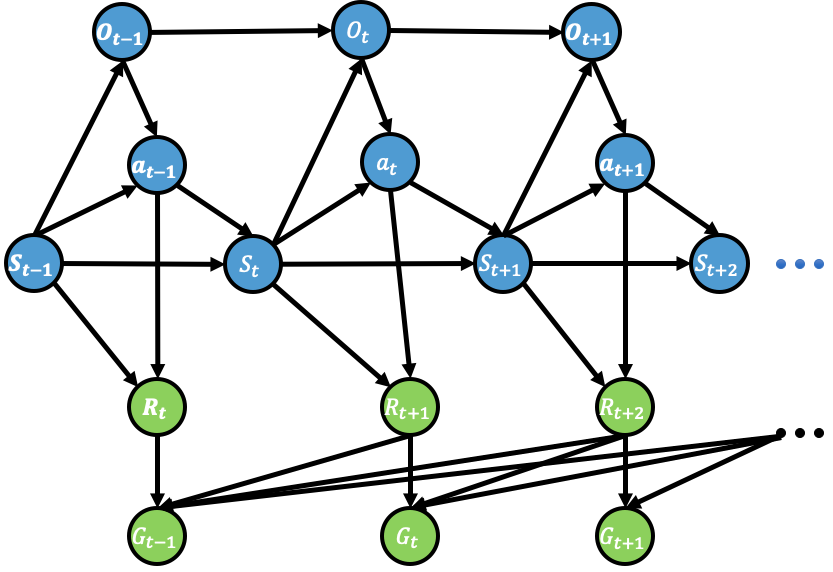
\includegraphics[width=0.45\linewidth]{./Part1/figures/doe.png}&
                                                              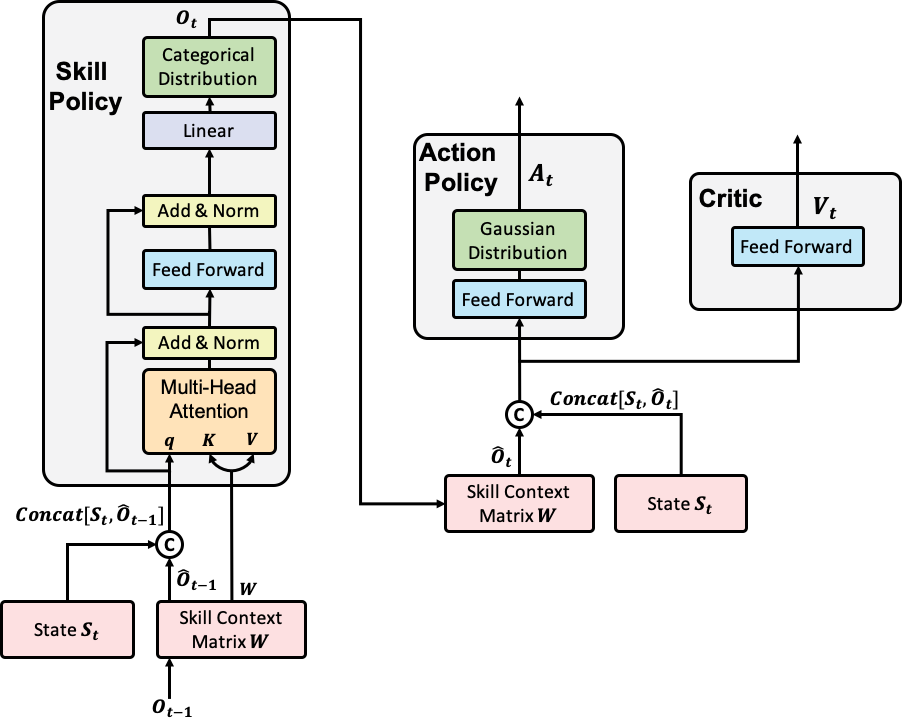
\includegraphics[width=0.45\linewidth]{./Part1/figures/sa_attn_net.png}\\
    {\small (a) PGM of SA}&
                            {\small (b) Network
                            Architecture of SA}\\
   
  \end{tabular}\vspace{-2mm}
  \caption{\label{fig:sa_net} The Skill-Action (SA) Architecture}
  \vspace{-6mm}
\end{figure*}

In this section, we define the dynamics (Markov process) of SA.
We first introduce MDP notations. A Markov decision process
$M=\{\sS,\sA,r,P,\gamma\}$ consists of a state space $\sS$, an
action space $\sA$, a state transition function
$P(\rvs_{t+1}|\rvs_t): \sS\rightarrow\sS$, a reward function
$r(\rvs,\rva):\sS\times\sA\rightarrow\sR$, and a discount factor
$\gamma\in\sR$. A policy $\pi=P(\rva|\rvs):\sS\rightarrow \sA$ is
a probability distribution defined over actions conditioning on
states. An expected discounted return is defined as $G_t =
\sum_k^N\gamma^kR_{t+k+1}$, where $R\in\sR$ is the actual reward
received from the environment. The value function
$V[\rvs_t]=\E_{\pi}[G_t|\rvs_t]$ is the expected return starting
at state $\rvs_t$ and following policy $\pi$ thereafter. The
action-value function is defined as $Q[\rvs_t,\rva_t]=
\E_{\tau_\pi}[G_t|\rvs_t,\rva_t]$. An Markov decision process
together with value functions defined on it are referred to as an
MDP~\cite{puterman2014markov}.

Having defined notations of MDP, we propose the dynamics of SA.
Specifically, a \textbf{skill index vector} $\rvo\in\sZ^M_2$ is
an $M$-dimensional one-hot vector, where $M$ denotes the total
number of skills to learn. Each entry $\ro\in\{0,1\}$ is a binary
random variable. $\ro_i=1$ means that the $i$-th skill is
activated. A \textbf{skill context matrix}
\cite{kosiorek2019stacked} $\mW_S\in \sR^{M\times E}$ is a
learnable parameter containing $M$ rows of $E$ dimensional real
vectors, the $i$-th row of $\mW_S$ corresponds to the $i$-th
skill $\ro_i$, and different columns encode different properties
of a skill. A \textbf{skill context vector} $\hat{\rvo}_t$ is
defined as:
\begin{equation}
  \label{eq:sa_skill_vector}
  \hat{\rvo}_t=\mW_S^{T}\cdot\rvo_t, \;\hat{\rvo}_t\in \sR^{E}.
\end{equation}
The \textbf{skill policy} is defined as:
\begin{equation}
  \label{eq:sa_o_p}
  P(\hat{\rvo}_t|\rvs_t,\hat{\rvo}_{t-1};\mW_s): \sS\times\sR^{E} \rightarrow \sR^{E},
\end{equation}
% todo: explain the functionality of P(o); what's the motivation;
% how is it implemented; advantages; contributions
which is a probability distribution over skill context vector
$\hat{\rvo}_{t}$ conditioned on state $\rvs_t$ and previous
sampled skill context vector $\hat{\rvo}_{t-1}$, with $\mW_S$ as
its learnable parameters.

The \textbf{action policy} is defined as:
\begin{equation}
  \label{eq:sa_a_p}
  P(\rva_t|\rvs_t,\hat{\rvo}_t): \sS\times\sR^E\rightarrow\sA,
\end{equation}
which is a probability distribution over the action random
variable $\rva_t\in\sA$ conditioned on the skill context vector
$\hat{\rvo}_t$ and state $\rvs_t$, and decodes them into primary
actions.

With both skill and action policies in hand, the dynamics of the
SA are defined as a Probabilistic Graphical Model
(PGM)~\cite{koller2009probabilistic} (Figure~\ref{fig:sa_net}
(a)):
\begin{align}
  \label{eq:sa_pgm_joint}
  \nonumber  P(\tau) = &P(\rvs_0)P(\hat{\rvo}_0)P(\rva_0|\rvs_0,\hat{\rvo}_0)\\
                       &\prod_{t=1}^\infty P(\rvs_t|\rvs_{t-1},\rva_{t-1})P(\hat{\rvo}_t|\rvs_t,\hat{\rvo}_{t-1})P(\rva_{t}|\rvs_{t},\hat{\rvo}_{t}),
\end{align}
where
$P(\tau)=P(\rvs_0,\hat{\rvo}_0,\rva_0,\rvs_1,\hat{\rvo}_1,\rva_1,\ldots)$
denotes the joint distribution of the PGM. Note that under this
formulation, $P(\tau)$ is actually an Hidden Markov Model (HMM)
with $\rvs_t$, $\rva_t$ as observable random variables and
$\hat{\rvo}_t$ as latent variables.

\subsection{MDP of the Skill-Action Architecture}
\label{sec:sa_mdp}

With SA's dynamics in hand, in this section, we first propose a
novel ``skill value upon arrival function'' and theoretically
prove that it has a smaller variance than the conventional value
function. This property is empirically justified in
Section~\ref{sec:exp_perf} and further discussed in
Appendix~\ref{sec:append_gist}. Then, we derive the recursive
formulation of value functions and formulate the MDP. Based on
the MDP, skill and action policies' gradients theorems are
finally derived.

Rather than use the conventional value function $V[\rvs_t]$, we
define the \textbf{skill value upon arrival function}
$V[\rvs_t,\hat{\rvo}_{t-1}]$ (derivations in Appendix
\ref{sec:appen_sa_v_proof}) as:
\vspace{-3mm}
\begin{equation}
  \label{eq:sa_v}
  V[\rvs_t,\hat{\rvo}_{t-1}]=\E[G_t|\rvs_t,\hat{\rvo}_{t-1}]= \sum_{\hat{\rvo}_t}P(\hat{\rvo}_t|\rvs_t,\hat{\rvo}_{t-1})Q_O[ \rvs_t,\hat{\rvo}_t].
\end{equation}
\begin{prop}
  \label{prop:var_unb}
  $V[ \rvs_t,\hat{\rvo}_{t-1} ]$ is an unbiased estimation of $V[ \rvs_t ]$.
\end{prop}
\begin{prop}
  \label{prop:var_red}
  The variance of $V[ \rvs_t,\hat{\rvo}_{t-1} ]$ is less than or equal to $V[ \rvs_t ]$.
\end{prop}
\vspace{-3mm}
\begin{proof}
  See Appendix \ref{sec:appen_sa_v_proof}
\end{proof}\vspace{-3mm}
Eq.~(\ref{eq:sa_v}) states that the skill value function upon
arrival is an expectation over skill value function
$Q_O[\rvs_t,\hat{\rvo}_{t}]$ conditioned on previous skill
$\hat{\rvo}_{t-1}$. The \textbf{skill value function}
$Q_O[\rvs_t,\hat{\rvo}_{t}]$ is defined as:
\begin{align}
  Q_O[\rvs_t,\hat{\rvo}_{t}]=\E[G_t|\rvs_t,\hat{\rvo}_{t}]
  \label{eq:sa_q_o}=\sum_{\rva_t}P(\rva_t|\rvs_t,\hat{\rvo}_{t})Q_A[ \rvs_t,\hat{\rvo}_t,\rva_t],
\end{align}
and the \textbf{skill-action value function} $Q_A[
\rvs_t,\hat{\rvo}_t,\rva_t]$ is defined as (derivations in
Appendix \ref{sec:appen_sa_v_proof}):
\begin{align}
\label{eq:sa_q_a}
Q_A[ \rvs_t,\hat{\rvo}_t,\rva_t]&=\E[G_t| \rvs_t,\hat{\rvo}_t,\rva_t]\nonumber\\
   &= r(s,a) + \gamma\sum_{\rvs_{t+1}}P(\rvs_{t+1}|\rvs_t,\rva_t)V[\rvs_{t+1},\hat{\rvo}_t],
\end{align}
where $\gamma \in \sR$ is a discounting factor. Expanding
(Eq.~\ref{eq:sa_q_a}) with (Eq.~\ref{eq:sa_v}) gives us a
recursion formulation from which Bellman equations and policy
gradient theorems are derived. To keep notations uncluttered, we
use $\theta_o$ to denote skill policy's parameters
(Eq.~\ref{eq:sa_o_p}) and $\theta_a$ to denote action policy's
parameters (Eq.~\ref{eq:sa_a_p}). The skill and action policies'
gradient theorems are:
\begin{thm}
  \textbf{ Skill Policy Gradient Theorem: } Given a stochastic skill policy
  differentiable in its parameter vector $\theta_o$, the gradient
  of the expected discounted return with respect to $\theta_o$ is:
  \begin{equation}
    \label{eq:sa_o_grad}
    \frac{\partial V[\rvs_t,\hat{\rvo}_{t-1}]}{\partial \theta_o}=\E[\;\frac{\partial P(\hat{\rvo}'|\rvs',\hat{\rvo})}{\partial \theta_o}Q_O[\rvs',\hat{\rvo}']\;|\;\rvs_t,\hat{\rvo}_{t-1}],
  \end{equation}
  ~where $\hat{\rvo}'$ is one time step later than $\hat{\rvo}$.
\end{thm}
\begin{thm}
  \textbf{ Action Policy Gradient Theorem: } Given a stochastic action policy
  differentiable in its parameter vector $\theta_a$, the gradient
  of the expected discounted return with respect to $\theta_a$ is:
  \begin{equation}
    \label{eq:sa_a_grad}
      \frac{\partial Q_O[\rvs_t,\hat{\rvo}_t]}{ \partial \theta_a }=\E[\;\frac{\partial P(\rva|\rvs,\hat{\rvo})}{\partial \theta_a}Q_A[ \rvs,\hat{\rvo},\rva]\; | \; \rvs_t,\hat{\rvo}_t].
  \end{equation}
 \vspace{-5mm} \begin{proof}
    See Appendix~\ref{sec:appen_sa_a_grad}
  \end{proof}\vspace{-3mm}
\end{thm}

% towrite:
%As conventional option frameworks, the action policy can also be
%composed of $M$ action policies, in which case all of our
%theorems still hold. However, 

Compared to MDP formulated algorithms, SMDP option frameworks are
sample inefficient and notoriously unstable to
hyperparameters~\cite{zhang2019dac}. The skill and action
policies' gradient theorems enable SA to be compatible with both
MDP on-policy and off-policy algorithms, and thus has much better
stability and convergence. This work is focused on deriving MDPs
of SA and its policy gradient theorems. To be comparable with
previous work \cite{zhang2019dac}, in this paper we directly
apply PPO~\cite{schulman2017proximal} to our learning algorithm
(Algorithm~\ref{alg:sa} in Appendix~\ref{sec:append_algo}).
Recent work \cite{wulfmeier2020data} shows that the off-policy
algorithm gives a performance boost to option variants. Designing
off-policy algorithms for SA remains open for future work.


\subsection{Networks Architecture}
\label{sec:net_arch}
\begin{figure*}[h]
  \centering
  \begin{tabular}{c}
    
\includegraphics[width=2\columnwidth]{Part1/figures/infinite_horizon.png}\\
    \vspace{-1mm}{\small (a) Infinite Horizon Environments}\\
    \includegraphics[width=2\columnwidth]{Part1/figures/finite_horizon_4.png}\\
    \vspace{-1mm}{\small (b) Finite Horizon Environments}
  \end{tabular}\vspace{-2mm}
  \caption{\label{fig:exp_dac} Episodic Returns. X-axis is time step. Y-axis is
    Episodic Return}
  \vspace{-4mm}
\end{figure*}
After deriving the MDP of SA, we present a simple neural network
implementation of the Skill-Action Architecture
(Figure~\ref{fig:sa_net}). Unlike the conventional SMDP option
framework, which employs a termination function and an SMDP
master policy to temporally extend the execution of an option, SA
implements the temporal extension functionality by employing the
Multi-Head Attention (MHA) mechanism~\cite{vaswani2017attention}
(due to page limitations, we briefly explain MHA in
Appendix~\ref{sec:appen_mha}). At each time step, the skill
policy $P(\hat{\rvo}_t|\rvs_t,\hat{\rvo}_{t-1};\mW_s)$ attends to
(measures the compatibility of) all skill context vectors in
$\mW_s$ according to $\rvs_t$ and $\hat{\rvo}_{t-1}$. If
$\hat{\rvo}_{t-1}$ still fits $\rvs_t$, then the skill policy
assigns a larger attention weight to $\hat{\rvo}_{t-1}$, thus has
a tendency to continue with it. Otherwise, a new skill with
better compatibility will be sampled. The action policy is as
simple as one decoder to decode $\hat{\rvo}_t$ and $\rvs_t$ into
primary actions $\rva_t$. The attention mechanism together with
skill context vectors enable SA to temporally extend skills even
in the absence of termination functions.

Specifically, a \textbf{skill policy} (Eq.~(\ref{eq:sa_o_p}))
uses a concatenation of current state $\rvs_t$ and previous skill
context vector $\hat{\rvo}_{t-1}$ as the query for MHA. Both key
and value matrices are the skill context matrix $\mW_S$. In this
way, we have:

\begin{align}
  \label{eq:sa_net_skill_concat}
  \hat{\rvs}_{t-1} &= linear(\text{Concat}[\rvs_t,\hat{\rvo}_{t-1}]),\\
  \label{eq:sa_net_skill_mha}
  \rvd^O_t &= \text{MHA}(\hat{\rvs}_{t-1},\mW_S,\mW_S),\\
  \label{eq:sa_net_skill_sample}
  \rvo_t &\sim Categorical(\rvo_t|\rvd^O_t),
\end{align}
where the $linear$ layer simply projects the concatenated vector
to $E$ dimension. MHA is employed to attend to (measures the
compatibility of) all skills in $\mW_s$ according to $\rvs_t$ and
$\hat{\rvo}_{t-1}$. The \textbf{skill density vector} $\rvd^O_t$
is then used as densities for a Categorical distribution
$P(\rvo_t|\rvd^O_t)$, from which the new one-hot \textbf{skill
  index vector} $\rvo_t$ is sampled from. We can retrieve the
\textbf{skill context vector} by $\hat{\rvo}_t =
\mW_S^T\cdot\rvo_t$. With the skill context vector $\hat{\rvo}_t$
in hand, the \textbf{action policy} can be designed as simple as
a multi-layer Feed-Forward Networks (FFN) decoder:
\begin{align}
  \label{eq:sa_net_action_concat}
  \rvd^A_t &= \text{FFN}(\rvs_t,\hat{\rvo}_{t}),\\
  \label{eq:sa_net_action_sample}
  \rva_t &\sim P(\rva_t|\rvd^A_t),
\end{align}
where $\rvd^A_t$ is a density vector and $P$ is an arbitrary
probability distribution (works for both discrete and continuous
situations).

Similar to \citename{zhang2019dac}, because of the \textbf{skill
  value upon arrival function} $V(\rvs_t,\hat{\rvo}_{t-1})$,
(Eq.~\ref{eq:sa_v}) is an expectation of the \textbf{skill value
  function} $Q_O[\rvs_{t},\hat{\rvo}_{t}]$ (Eq.~\ref{eq:sa_q_o}).
It is sufficient for us to model only one critic function:
\begin{equation}
  \label{eq:nn_o_input}
  Q_O=\text{FFN}(\rvs_t,\hat{\rvo}_t),
\end{equation}
where $Q_O$ is implemented as a multi-layer FFN. We summarize the
detailed learning procedures in Algorithm~\ref{alg:sa} in
Appendix~\ref{sec:append_algo}.

Since $\hat{\rvo}_t$ encodes all context of a skill, SA only
needs one action policy decoder to decode the activated skill
context vectors $\hat{\rvo}_t$ and current state $\rvs_t$ into
primary actions $\rva_t$. This design choice largely improves the
scalability of SA: adding one more skill is as cheap as adding a
skill context vector. Moreover, unlike the option framework, in
which only the activated option's action policy gets updated, the
action policy learns to decode each dimension of skill context
vectors at every time step. This design choice largely improves
sample efficiency and enables SA to converge faster than the
conventional option framework.

% todo: layer by layer training
% todo: training layer by layer proof
\section{Learning Skills at Multi-levels of Granularity}
\label{sec:append_gist}

Implementations of the option framework share some common
limitations. When proposing the option framework,
\citename{sutton1999between} expected that learning at
multi-level of temporal abstraction should be in favor of faster
convergence and better exploration. On the contrary, significant
improvements on single task environments have not been witnessed
in most option
implementations~\cite{klissarov2017learnings,smith2018inference,harb2018waiting,zhang2019dac}.
To the best of our knowledge, SA is the first option
implementation in which these properties are significantly
witnessed but only on infinite horizon environments. In this
section, we address this problem by first giving a theoretical
explanation of why the value function is the main reason for this
deficiency in section~\ref{sec:append_turkey} and how
\textbf{deep wide value functions} could solve this problem. We
then thoroughly explain the motivations of SA, and why it is a
promising candidate for a deep wide framework, in
section~\ref{sec:append_dwsa}. We also give a further explanation
of how SA is connected to causality reinforcement learning
literature and how a temporal causal reward can be used in
objective to further solve this problem in
section~\ref{sec:append_causal_rew}.

\subsection{Problem Statement and Evidences}
\label{sec:append_turkey}

The expectation of improvements of the option framework on single
task environment builds on an assumption that, by exploiting
hierarchical action and state space, an agent's searching space
can be greatly reduced thus accelerates learning and improving
exploration. However, as reported in section~\ref{sec:exp_ext},
most option frameworks including SA suffer from ``the dominant
skill problem'' \cite{zhang2019dac} which prevents option
frameworks from effectively learning hierarchy in action and
state space as well as coordinating between skills.

One root reason for this problem is that conventional value
functions $V[S_t]$ and $Q[S_t,O_t,A_t]$ make values depend on
temporal latent variables indistinguishable (i.e. Although
different skills $o_1$ and $o_2$ results to different values,
such as $V[S_t,O_{t-1}=o_1]=10$ and $V[S_t,O_{t-1}=o_2]=-10$.
Because they arrive at the same state $S_t$, they have identical
values under conventional value function $V[S_t]=0$). This
deficiency makes option frameworks can only learn skills at very
coarse level thus fail to exploit hierarchical information. The
solution is to use a \textbf{deep wide value function}: enabling
the framework to learn fine-grained skills at mutli-levels of
granularity (deep) and making value functions depend on latent
variables with longer (wide) dependencies (e.g. $V[S_t,O_{t-1}]$
and $Q[S_t,O_t,A_t,O_{t-1}]$).

To have a better understanding the importance of the deep wide
value function, let us consider a simple environment which can be
easily solved by $Q[s_t,a_t,a_{t-1}]$ but not $Q[s_t,a_t]$.

Suppose we are training a robot which only has a camera sensor to
cook thanksgiving turkey. In this setting there are only two
states: $\sS=\{\text{Raw Turkey Image},\text{Cooked Turkey
  Image}\}$. The robot's action space only consists of two
actions: $\sA=\{\text{Stuff turkey},\text{Roast turkey}\}$. As
for reward, if the robot roasted a stuffed turkey, then the
reward is $10$. However, if the robot roasted an un-stuffed
turkey, then the reward is $-10$. The $\text{stuff turkey}$
action receives $0$ reward.

The difficulty in this environment is, since the robot only has a
camera to capture an image of the turkey, it can only observes
either $\{\text{Raw Turkey Image}\}$ or $\{\text{Cooked Turkey
  Image}\}$. There is no way to look inside the turkey and see if
the turkey is stuffed. Under this setting, a robot can never
learn to first stuff a turkey and then roast it because
$Q[\text{Raw Turkey Image},\text{Stuff Turkey}] = Q[\text{Raw
  Turkey Image},\text{Roast Turkey}] = 0$. Therefore, the robot
can only randomly cook a turkey. However, this problem can be
easily solved by using a deep wide value function
$Q[S_t,A_t,A_{t-1}]$.

The core problem in this setting is, action has no effect on
states, it only affects rewards. At the first glance this is a
Partially Observed MDP (POMDP) problem since the state of whether
the turkey is stuffed is un-observed. This is true in all
reinforcement learning settings without dependencies on latent
variables. However, it goes much deeper in HRL settings.

In HRL, a common formulation is to estimate a latent variable $O$
to encode hierarchical information and makes the policy depends
on it $P(A_t|S_t,O_t)$. Since $O$ is a latent variable, it is
highly likely that at state $S_t$, different latent variable
$P(A_t|S_t,O_t=o_x)$ and $P(A_t|S_t,O_t=o_y)$ emits the same
action $A_t=A_1$, and thus makes the conventional value function
indistinguishable between $o_x$ and $o_y$.

This phenomenon is especially common around the switching time
step of two skills: around switching point, states are usually
compatible with both old and new skills. Conventional value
functions will be especially confused at those moments. This is
exactly what we observed in Figure~\ref{fig:skill_sequence}:
overall, skill 2 is executed consistently. However, there are
some random switches to skill 1. And the randomization is
increased between around switching time steps. To explicitly show
this, we visualized ``Run4'' into a video:
$\text{https://www.youtube.com/watch?v=QiLVZvI6NJU}$. The skill
selection is very random at the beginning of the episode as well
as around the switching point (the 16th second). These are
exactly the most confusing moments of conventional value
functions. This is not a cherry-pick result but a common problem.
Similar patterns can also be observed here
$\text{https://youtu.be/xrfxbI3duBM?t=4}$ in a HumanoidStandUp
environment.

Due to the insufficiency of conventional value functions,
compatible states have to be different enough to cause
distinguishable values of value functions. Therefore, with
conventional value functions, SA is only able to learn very
coarse skills. For example, as shown in
Figure~\ref{fig:interp_joint} and the video, the HalfCheetah
agent is only able learn two skills: one is to run forward, one
is to stand up when fall. However it is not able to learn more
fine-grained skills such as jump forward and landing. This
problem is not limited to SA, but is a common problem in HRL. The
solution is to use deep wide value functions.

\subsection{Motivations behind SA's Architecture}
\label{sec:append_dwsa}

SA is carefully designed to make the most out of deep wide value
functions. Compared to other HRL frameworks, SA has following
advantages: 

\begin{enumerate}
\item Stable and unbiased estimation: Thanks to
  proposition~\ref{prop:var_unb} and \ref{prop:var_red}, the
  higher the order of the MDPs, the smaller the variance will be.
  The deep wide value functions stays unbiased estimations of
  conventional value functions no matter how many dependencies
  introduced. The current solution in option framework is a
  biased estimation \cite{harb2018waiting} and adding
  hyper-parameters to the framework.
\item Easy to incorporate wide value functions: Incorporating a
  deep wide value function is straightforward, SA's \textbf{skill
    value upon arrival function} is already a wide function. The
  \textbf{skill value function} and the \textbf{skill-action
    value function} can be easily extended to wide function by
  adding a first-order dependency on $\hat{O}_{t-1}$.
\item Easy to incorporate deep value functions: SA is MDP
  formulated, extending SA to multiple hierarchies is
  straightforward.
\item Scalability to long time dependencies: SA is MDP
  formulated, adding more time dependencies is simply to change
  the 1st-order MDP to higher-order MDPs while both value
  functions and gradient theorems stay unchanged; SA is attention
  based, SA can easily attends to thousand time steps without
  adding any extra complexity to neither skill policy nor action
  policy.
\item Scalability to multiple hierarchies of skills: SA is
  attention based and embedding based. Adding skills is as simple
  as adding skill context matrix. In traditional option
  frameworks \cite{riemer2018learning}, the number of option
  (note that each option is a neural network) grows at $O(N^L)$
  complexity of levels ($N$ is the number of options and $L$ is
  the number of levels).
\item Interpretability. As shown in section~\ref{sec:interpret},
  skill context vectors learned under SA-based architectures are
  straightforward to visualize and interpret. This property is
  especially useful for investigating multi-level granularity
  skills.
\end{enumerate}

\subsection{Causality Discovery Rewards}
\label{sec:append_causal_rew}

Although theoretically a DWSA can learn multi-level granularity
skills, on-policy optimization algorithm is often insufficient
for learning such models especially in sparse reward
environments. However, SA has a natural connection with causal
reinforcement learning thus can exploits causality as a reward in
objective function to further facilitate fine grained skill
discovery. In this section we explain how skill embedding vectors
learned by SA encodes temporal causality relationships and how to
use them to devise causal rewards.

In causal reinforcement learning area, \citename{doshi2016hidden}
proposed Hidden Parameters MDP (Hi-MDP) in which a skill vector
like hidden parameter vector is introduced to learn abstract
properties from environments. PEARL \cite{rakelly2019efficient}
utilizes meta-learning framework to learn a skill representation
that encodes abstract properties of a task and updates the
framework in an off-policy manner to improve sample efficiency in
transfer learning. \citename{killian2017robust} extended Hi-MDP
by including the hidden parameter vector into transition
probability function. \citename{perez2020generalized} further
extended their work by proposing Generalized Hidden Parameter
MDPs (GHP-MDPs), a causality discovery framework by including
hidden parameter vector into both transition function and value
function.

GHP-MDPs is a special case of SA with number of skills $M=1$.
When $M>1$, SA not only encodes causality relationships between
environments and actions but also temporal causality between
skills. Since the latent variable is modeled as a skill vector,
the distance between different trajectories is straightforward to
be calculated and thus can be used as a causal reward to
encourage fine-grained and disentangled skills' discovery. To the
best of our knowledge, SA is the first RL framework concerns
causality in temporal abstraction sequences. We focus this paper
on proposing SA, the causality rewarded SA will be discussed in
future works.

Another interesting understanding of SA is that, rather than an
implementation of the option framework, SA can also be seen as a
novel capsule network~\citename{kosiorek2019stacked} trained by
policy gradient theorems. In Stacked Capsule Auto-Encoders (SCAE)
\cite{kosiorek2019stacked}, a ``capsule'' vector encodes a
different property (scale, orientation, etc.) of the visual
object in each dimension. \citename{kosiorek2019stacked} proposed
to delegate the complexity of part objects detection and
part-to-whole objects aggregation by employing the attention
mechanism \cite{lee2019set} on which a generative model is then
built to further decode the whole-part relationships. This design
choice abstracts the complexity of inference away from the
decoder and largely simplified the designation of the generative
model.

In this paper, we follow their motivations of learning better
representations and utilizing the attention mechanism to simplify
the inference problem (sampling new skill without termination
function). Moreover, the skill context vector is analogously to a
capsule and the skill-action relationship is analogously to the
whole-part relationship in the SCAE. Similar to SCAE utilizing
the equi-variance property of the whole-part relationship to
achieve computing efficiency and better performance, it will be
very exciting to investigate potentially ``equi-variance'' or
``invariance'' properties existed in skill-action relationships,
which might give rise to a novel causal inference architecture in
the reinforcement learning area.

\section{Experiments Results}
\label{sec:append_exp}
\subsection{Performance}
\label{sec:append_exp_perf}

In this section we provide results for all ten OpenAI Gym Mujoco
Environments. Those environments can be classified into two categories:
infinite horizon environments (i.e., HalfCheetah, Swimmer,
HumanoidStandup and Reacher) and finite horizon environments (the
other).
\begin{figure*}[thb]
  \centering
  \includegraphics[width=1\linewidth]{./Part1/figures/all_exps.png}\\
  \caption{\label{fig:all_tasks} Performance of Ten OpenAI Gym
    MuJoCo Environments.}
\end{figure*}

\begin{table*}[]
\caption{Performance of Infinite Horizon Environments}
\label{table:single_infinite}
\vskip 0.15in
\begin{center}
\begin{tabular}{|l|l|l|l|l|}
\hline
        & HalfCheetah        & Swimmer           & HumanoidStandup     & Reacher          \\ \hline
PPO     & 2143.6                & 59.9                 & 62262.2                & -7.5                \\ \hline
DAC+PPO & 1830.1                & 85.0                 & 38954.9                & -8.1                \\ \hline
AHP+PPO & 1701.7                & 86.7                 & 38684.9                & -7.3                \\ \hline
PPOC    & 1441.2                & 43.6                 & 39841.7                & -9.4                \\ \hline
OC      & 832.3                 & 33.0                 & 52352.7                & -15.3               \\ \hline
SA+PPO  & {\ul \textbf{3446.7}} & {\ul \textbf{107.8}} & {\ul \textbf{91654.5}} & {\ul \textbf{-4.6}} \\ \hline
\end{tabular}
\end{center}
\vskip -0.1in
\end{table*}

\begin{table*}[]
\caption{Performance of Finite Horizon Environments}
\label{table:single_finite}
\vskip 0.15in
\begin{center}
\begin{tabular}{|l|l|l|l|l|l|l|}
\hline
        & Walker2d           & Hopper             & InvertedPendulum  & InvertedDoublePendulum & Ant                & Humanoid          \\ \hline
PPO     & 1512.5                & 1489.9                & 939.9                & 7112.6                    & 1049.6                & 562.1                \\ \hline
DAC+PPO & {\ul \textbf{1968.0}} & 1702.2                & {\ul \textbf{943.7}} & 5804.5                    & 985.8                 & 487.6                \\ \hline
AHP+PPO & 1520.6                & {\ul \textbf{1993.6}} & 940.0                & {\ul \textbf{7120.7}}     & {\ul \textbf{1359.3}} & {\ul \textbf{569.3}} \\ \hline
PPOC    & 756.1                 & 1308.1                & 936.2                & 7117.6                    & 429.4                 & 483.9                \\ \hline
OC      & 391.9                 & 487.6                 & 207.1                & 2369.4                    & 433.4                 & 475.1                \\ \hline
SA+PPO  & 1856.9                & 1955.3                & 906.5                & 6884.1                    & 907.4                 & 528.7                \\ \hline
\end{tabular}
\end{center}
\vskip -0.1in
\end{table*}

\newpage
\subsection{Temporal Extension}
\label{sec:append_exp_ext}

In Figure~\ref{fig:duration}, we plot the average duration of
each skill during 430 training episodes (each episode contains a
trajectory of 512 time steps) of the HalfCheetah environment. In this
environment, the agent learns to run half of a Cheetah by controlling 6
joints: back thigh, back shin, back foot, front thigh, front
shin, and front foot. The faster the Cheetah runs forward, the
higher return it gets from the environment. At the start of
training, all skills' durations are short. After the $100$-th
episode, Skill 2's duration quickly grows and dominates the
entire episode. The dominant skill phenomenon is also reported in
other option implementations such as DAC. One explanation for
this domination phenomenon is that for some single task environments,
primitive actions might be enough to express the optimal policy,
in which case extra levels of abstraction (skills) become
overhead. However, because the duration of dominant skill starts
to fall at the end of training and SA significantly outperforms
PPO which only employs primary actions, these facts indicate that
SA has a better capability of automatically discovering abstract
actions from primary actions as well as coordinating between
them.
\begin{figure*}[thb]
  \centering
  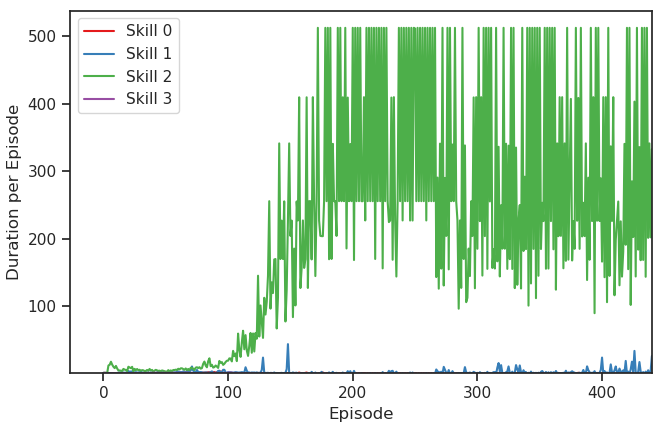
\includegraphics[width=0.7\linewidth]{./Part1/figures/duration.png}\\
  \caption{\label{fig:duration} Duration of 4 options during 430
    training episodes of HalfCheetah.}
\end{figure*}

To illustrate how SA coordinates
skills, we take the HalfCheetah model trained after 1 million
steps and independently run it 4 times (4 episodes. each episode
contains 512 time steps). Skill activation sequences of 4 runs
are then plotted in Figure~\ref{fig:option_pattern}.
\begin{figure*}[thb]
  \centering
  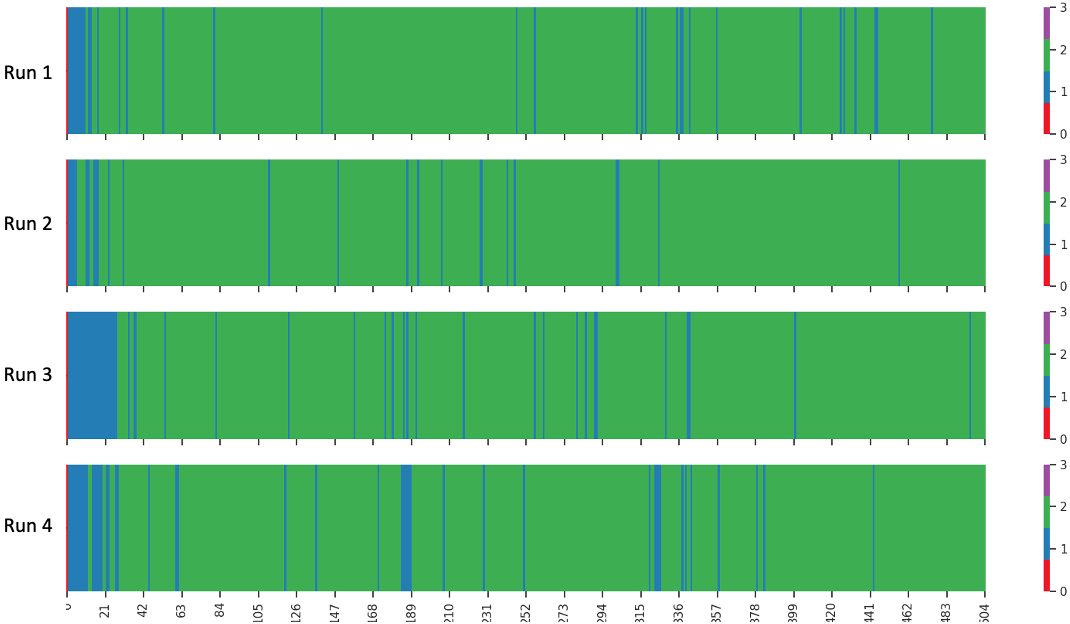
\includegraphics[width=0.7\linewidth]{./Part1/figures/option_pattern.png}\\
  \caption{\label{fig:option_pattern} Activated option sequences
    of 4 independent HalfCheetah runs.}
\end{figure*}
As we can see that there are some common patterns between all 4
independent runs. For example, all runs start with Skill 0 and
use Skill 1 at the early stage. After executing Skill 1 for a
short period, they all switch to Skill 2 which has longest
durations in all 4 runs. From time to time they will fall back to
Skill 1 for short periods and quickly switch to Skill 2 again.
This pattern of coordination indicates that Skill 1 and Skill 2
have completely different functionality and SA has the capability
of automatically discovering as well as leveraging those
skills.

\subsection{Interpretation of Skill Context Vectors}
\label{sec:append_interpret}

In this section we continue with the HalfCheetah model used in
Section~\ref{sec:append_exp_ext} and demonstrate how to interpret
skill context vectors as well as skill activation sequences
(Figure \ref{fig:option_pattern}). In HalfCheetah, the agent
learns to run half of a Cheetah by controlling 6 joints: back
thigh, back shin, back foot, front thigh, front shin, and front
foot. The faster the Cheetah runs forward, the higher return it
gets from the environment. We interpret skill context vectors and
activation patterns by first inspecting what property each
dimension of the skill context vector encodes (Figure
\ref{fig:first_dim_perturb}). Once each dimension is understood,
skills (Figure \ref{fig:all_skill_vectors}) become straight
forward to interpret by simply inspecting on which dimension
(property) they have the most significant weights (Figure
\ref{fig:interp_skill}). These interpretations can further be
taken to explain skill activation patterns in Figure
\ref{fig:option_pattern}.
\begin{figure*}[thb]
  \centering
  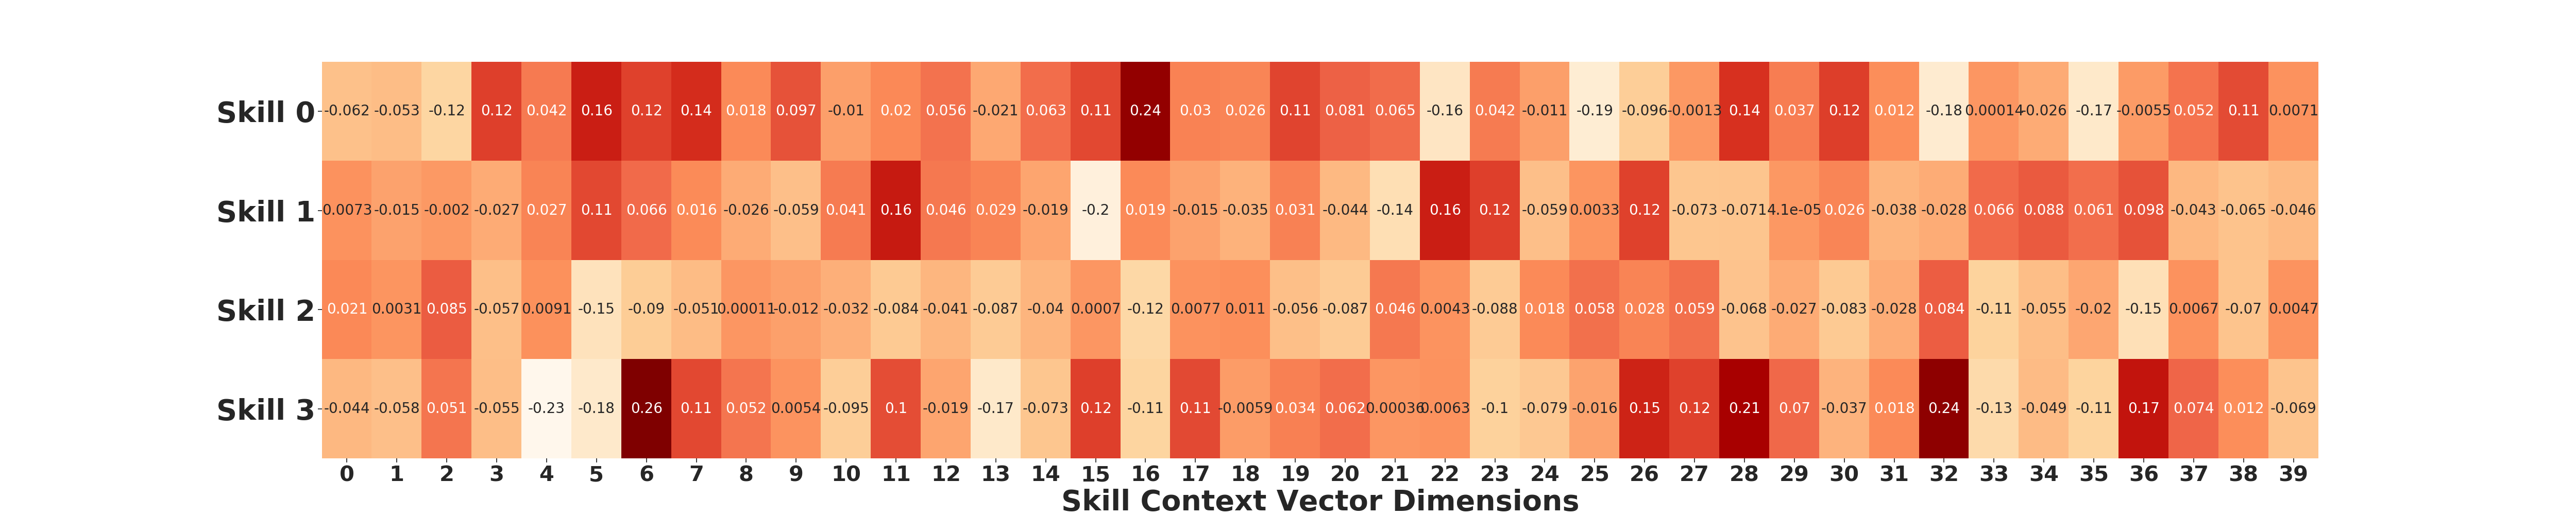
\includegraphics[width=1\linewidth]{./Part1/figures/all_skill_vectors.png}\\
  \caption{\label{fig:all_skill_vectors} Heatmap of all 4 skill
    context vectors}
\end{figure*}

As the first step, we follow \citename{sabour2017dynamic} to
interpret what property each dimension of the skill context
vector in Figure~\ref{fig:all_skill_vectors} encodes by
perturbing each dimension and decode perturbed skill context
vectors into primary actions. Specifically, we perturb one
dimension by adding a range of perturbations $[{-0.1}, 0.09]$ by
intervals of $0.01$ onto it while keep the other dimensions
fixed. After perturbation, each skill context vector dimension
has $20$ perturbed vectors. We then use the action policy decoder
to decode all those vectors into primary actions and see how the
perturbation affects the primary action. As an illustration, we
plot Dimension 0's all $20$ perturbed results in Figure
\ref{fig:first_dim_perturb}.
\begin{figure*}[thb]
  \centering
  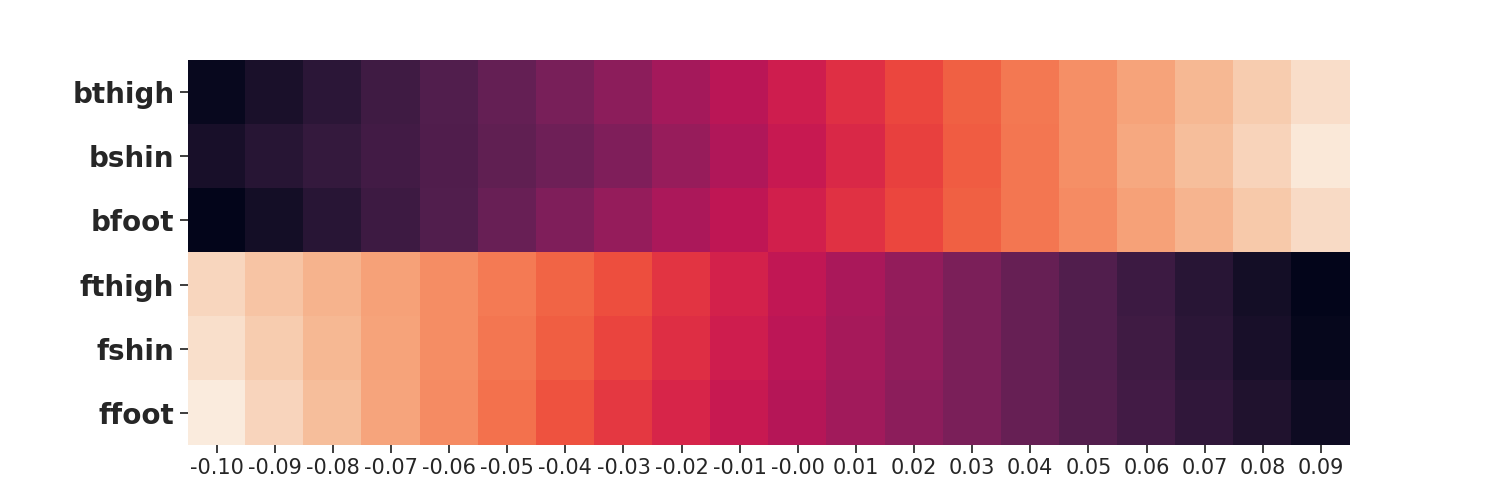
\includegraphics[width=1\linewidth]{./Part1/figures/skill_heatmap.png}\\
  \caption{\label{fig:first_dim_perturb} Perturbation on the
    Dim 0}
\end{figure*}

With visualization of perturbation results in hand, we can
interpret what property each dimension encode by inspecting
relationships between perturbations and primary actions. In
Figure \ref{fig:first_dim_perturb}, as an example, it is clear
that changes on Dim $0$ has opposite effect on the back leg and
front leg: a larger value on Dim $0$ will assign the back leg a
larger torque while the front leg a smaller one, and vice versa.
This means Dim $0$ is has a focus point property: it focuses
torque on only one leg.

Once we know how to interpret one dimension, we can move on to
interpret the whole skill context vector. Since Skill $1$ and
Skill $2$ are two main skills employed in
Figure~\ref{fig:option_pattern}, here we provide an example of
how to interpret them. Figure~\ref{fig:all_skill_vectors} shows
that Skill $1$ has significant values on dimension $11$, $15$ and
$22$. Skill $2$ is significant on dimension $2$, $5$ and $36$. We
demonstrate these dimensions in the same manner as
Figure~\ref{fig:first_dim_perturb} below:
\begin{figure*}[thb]
  \centering
  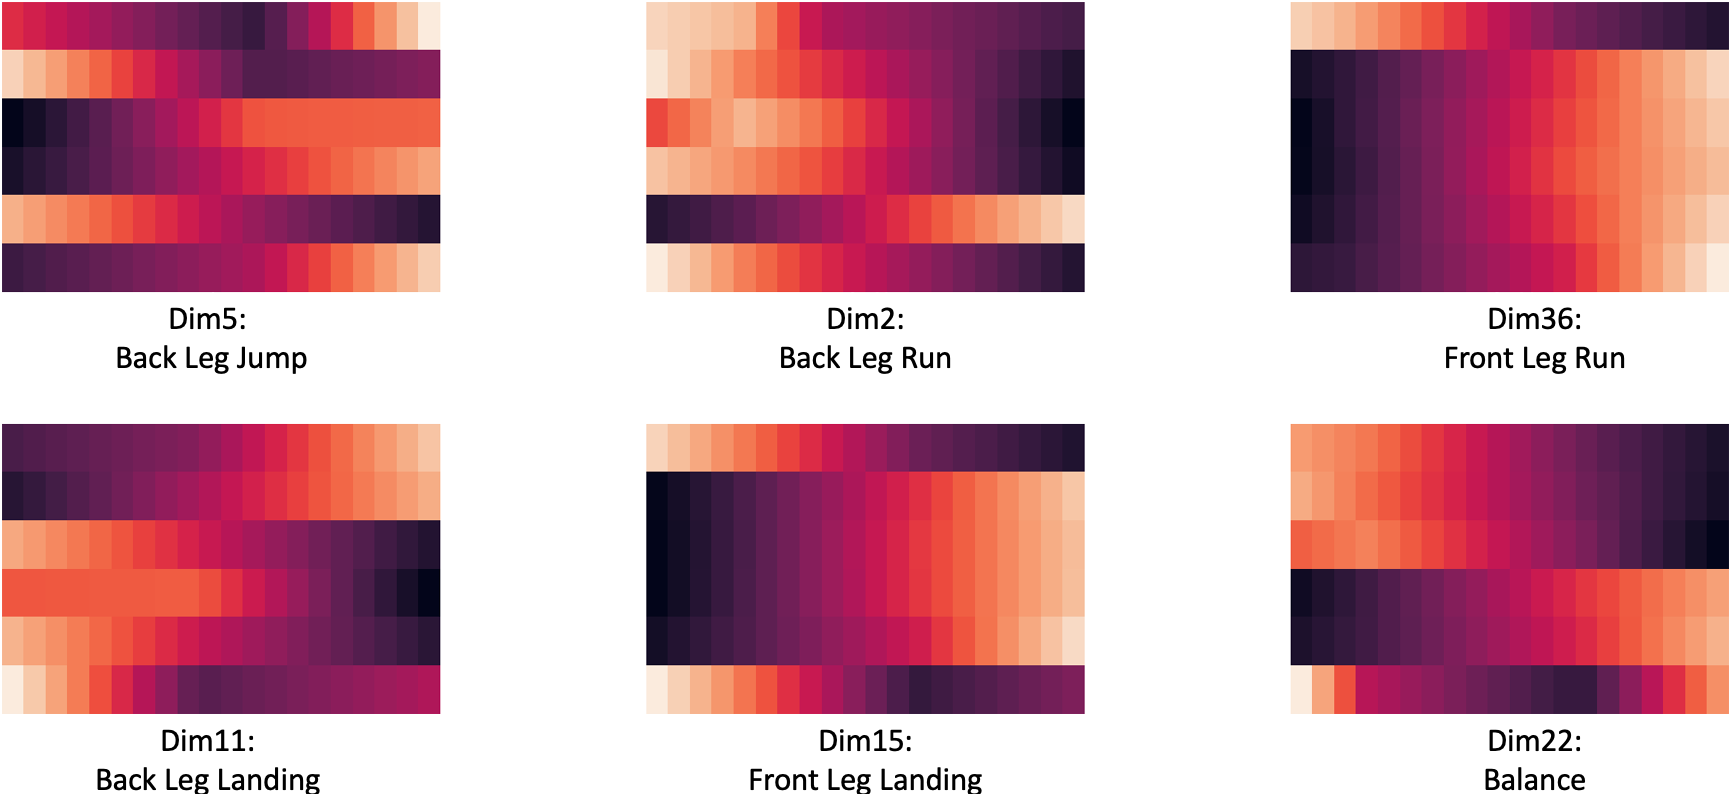
\includegraphics[width=1\linewidth]{./Part1/figures/interp_2_skills.png}\\
  \caption{\label{fig:interp_skill} Interpretation of Skill 1
    and Skill 2}
\end{figure*}

Subfigures in Figure~\ref{fig:interp_skill} can be interpreted in
the same manner as Figure~\ref{fig:first_dim_perturb}. As an
example, from Figure~\ref{fig:all_skill_vectors} we can see that
Skill $1$ has a significant small value on Dim $11$. In
Figure~\ref{fig:interp_skill}, it shows that a smaller Dim $11$
will twist the front leg forward and back foot forward while
twist back thigh, back shin backward. Composition of these
movements is a back leg landing property. Similarly, we can
interpret that Dim $15$ is a front leg landing property and Dim
$22$ is a balancing property. Therefore, Skill $1$ is focusing on
landing from all positions.

Unlike other skill context vectors which have apparent focusing
dimensions, Skill $2$ has a rather balanced skill context vector.
It has no apparently dominant dimension. It only has slightly
more significant values on Dim $2$, $5$, $36$, which are focusing
on jumping and running properties. Therefore, Skill $2$ is more
like an ``all-weather'' skill: it is a skill having very balanced
properties with a slightly demonstration on running and jumping.

Interpretations of Skill $1$ and $2$ above can then be taken to
understand skill activation patterns in
Figure~\ref{fig:option_pattern}: as an all-weather skill, Skill
$2$ is the most frequently executed one and has the longest
duration. From time to time, when the Cheetah needs to land and
balance itself, Skill $1$ will be executed. However, since
landing skill does not provide power of moving forward and thus
has lower returns to continue, once the body is balanced the
Cheetah will quickly stop Skill $1$'s execution and keep running
with Skill $2$.

\subsection{Transfer Learning Results}
\label{sec:append_transfer}

\begin{table*}[h]
\caption{Performance of Deepmind Control Suite Transfer Learning Environments}
\label{table:transfer}
\begin{center}
\begin{tabular}{|l|l|l|l|l|l|l|}
\hline
        & CartPole             & Reacher              & Cheetah              & Fish                 & Walker1              & Walker2              \\ \hline
PPO     & 829.7                & 327.6                & 73.0                 & 287.9                & 231.8                & 72.2                 \\ \hline
DAC+PPO & 970.8                & 517.2                & 211.2                & 505.4                & {\ul \textbf{590.3}} & 360.5                \\ \hline
AHP+PPO & 966.5                & 395.2                & 167.4                & 357.9                & 362.1                & 143.2                \\ \hline
PPOC    & 942.1                & 400.1                & 72.7                 & 336.7                & 236.6                & 80.9                 \\ \hline
OC      & 106.1                & 19.4                 & 100.6                & 286.6                & 356.3                & 238.7                \\ \hline
SA+PPO  & {\ul \textbf{974.1}} & {\ul \textbf{675.3}} & {\ul \textbf{233.8}} & {\ul \textbf{562.1}} & 473.8                & {\ul \textbf{403.0}} \\ \hline
\end{tabular}
\end{center}
\end{table*}

\section{MDP Equivalence to the SMDP Option Framework}
\label{sec:appen_oc_pgm}

In this section, we show that the the conventional Semi-Markov
Decision Problem (SMDP) option framework which employs Markovian
options actually has an MDP equivalence. We first follow
\citename{bishop2006pattern}'s method and formulate the dynamics
of the option framework as an Hidden Markov Model
(HMM)~\cite{bishop2006pattern} in section~\ref{sec:appen_hmm}.
With Probability Graphical Model (PGM)~\cite{bishop2006pattern}
and its conditional independence relationships (Chapter 8.2.1
\cite{bishop2006pattern}) in hand, we then move on to prove that
MDP formulation has identical value functions
(section~\ref{sec:appen_mdp}), bellman equations as well as
intra-option policy and termination policy gradients to SMDP
formulation (section~\ref{sec:appen_mdp_grad}). To the best of
our knowledge, this is the first work discovering the option
framework's MDP equivalence and deriving the option framework
from a PGM view.

\subsection{Background: The Option Framework}
\label{sec:appen_oc_background}

\citename{sutton1999between} proposed the option framework to
demonstrate the temporal abstraction problem. A scalar
$\ro\in\sZ$ denotes the index of an option where $\sO \subseteq
\{1,2,\ldots,M\}$ and $M$ is the number of options. An Markovian
option is a triple $(\sI_{o},P_{o}(\rva|\rvs),P_{o}(\rb|\rvs))$
% $(\sI_{o_t},P_{o_t}(\rva_t,|\rvs_t),P_{o_t}(\rb_t|\rvs_t))$
in which $\sI_{o}\subseteq\sS$ is an initiation set where the
option $o$ can be initiated. $P_{o}(\rva|\rvs):\sS\rightarrow\sA$
is the intra-option policy which maps environment states
$\rvs\in\sS$ to an action vector $\rva\in \sA$.
$P_{o}(\rb|\rvs):\sS\rightarrow\sZ_2$ is a termination function
where $\rb$ is a binary random variable. It is used to determine
whether to terminate ($\rb=1$) the policy $P_{o}(\rva|\rvs)$ or
not ($\rb=0$). Conventionally, $\beta_o=P_o(\rb=1|\rvs)$. Since
an option's execution may persist over a variable period of time,
a set of options' execution together with its value functions
constitutes a Semi-Markov Decision Problem (SMDP)
\cite{puterman2014markov}. When an old option is terminated, a
new option will be sampled from the master policy
(policy-over-options) $o\sim P(o_{t+1}|\rvs_{t+1}):
\sS\rightarrow\sO$.
\begin{figure*}[th!]
  \centering
  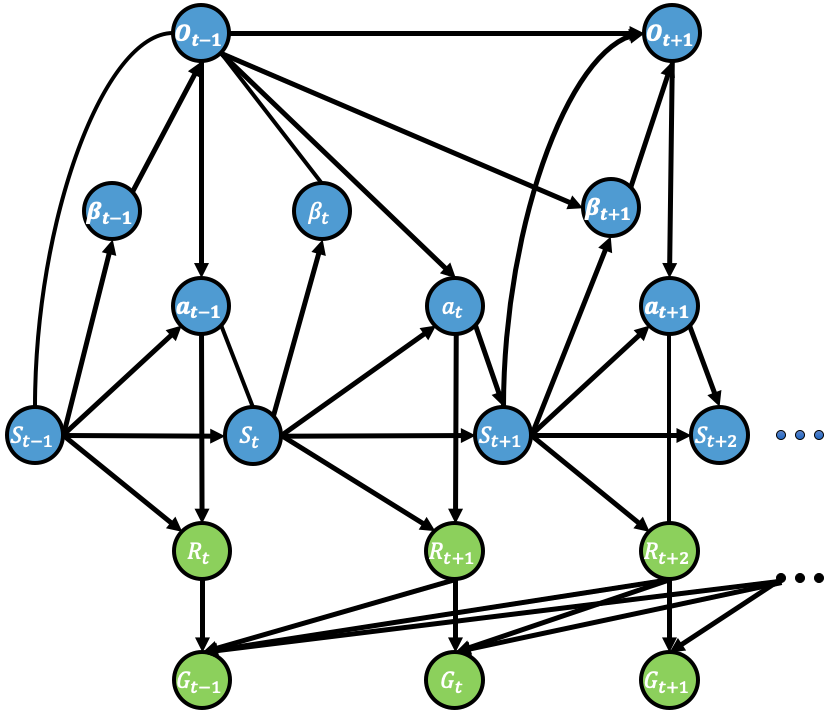
\includegraphics[width=0.5\linewidth]{Part1/figures/oc_smdp.png}\\
  \caption{\label{fig:oc_smdp} An Illustration of the SMDP Option
    Framework. An option $\ro_{t-1}$ is selected by
    master policy $P(\ro_{t-1}|\rvs_{t-1})$ at time step
    $t-1$. At time step $t$, termination function
    $\beta_{o_{t-1}}(\rvs_t)$ determines to continue option
    $\ro_{t-1}$. So that there is no random variable $\ro_t$ at
    time step $t$ compared to there are random variables $\rvo$
    at every time step in MDP formulation
    (figure~\ref{fig:oc_pgm}).}
\end{figure*}
Due to the SMDP formulation, an option can only be improved when
the option terminates. We refer this as the SMDP-style learning
which is sample inefficient and prevents applying SOTA MDP based
algorithms such as the Proximal Policy Optimization (PPO)
algorithm \cite{schulman2017proximal}.



\subsection{HMM dynamics for the Option Framework}
\label{sec:appen_hmm}

We follow \citename{bishop2006pattern}'s formulation of mixture
distribution and Probabilistic Graphical Models (PGMs). By
introducing option variables as latent variables and adding extra
dependencies between them, we show that the conventional SMDP
version of the option framework
\cite{bacon2017option,sutton2018reinforcement,sutton1999between,harb2018waiting,zhang2019dac}
has an MDP equivalence.
\begin{figure*}[th!]
  \centering
  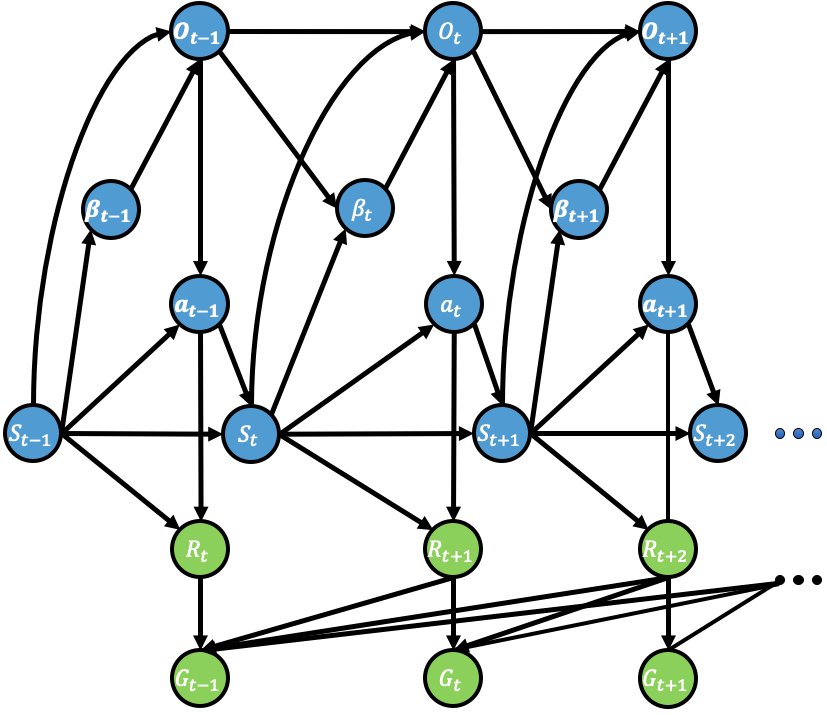
\includegraphics[width=0.5\linewidth]{Part1/figures/oc_pgm.png}\\
  \caption{\label{fig:oc_pgm} PGM of the MDP Option Framework}
\end{figure*}
Following \citet{bishop2006pattern}'s notation, we use bolded
letter $\rvs\in\sS$ to denote a random variable and normal letter
$\rs$ to denote its realization. Without special clarification, a
random vector can have either a vector of continuous or discrete
entries. Vector $\rvo\in\sO$ is an $M$-dimensional one-hot vector
and each entry $\ro\in\{0,1\}$ is a binary random variable.
$P(\rvo_t|\rvs_t)$ denotes the probability distribution over
one-hot vector $\rvo$ at time step $t$ conditioned on state
$\rvs_t$. $P(\rvo_t=\ro_t|\rvs_t)$ denotes a probability entry (a
scalar value) of the random variable $\rvo_t$ with a realization
at time step $t$ where $\ro_t=1$ and $\ro\in\rvo_t/\ro_t=0$.
% todo: define an option set P_o(a) P_o(b) I

In figure~\ref{fig:oc_pgm}, $\rvs\in\sS$, $\rvo\in\sO^M$,
$\rvb\in\sB^M$ and $\rva \in \sA$, denote the state, option,
termination and action random variable respectively. $\rvo$ is an
$M$-dimensional one-hot vector and $\rvb$ is an $M$-dimensional
binary vector where each entry $\rb\in\{0,1\}$. $M$ is the number
of options. $R_{t+1}$ is the actual reward received from the
environment after executing action $\rva_{t}$ in state $\rvs_t$.
$G_t=R_{t+1}+\gamma R_{t+2}+\gamma^2R_{t+3}\cdots$ is the
discounted expected return where $\gamma\in \sR$ is a discount
factor.

The termination policy distribution
$P(\rvb_t|\rvs_t,\rvo_{t-1}):\sS\times\sO\rightarrow\sB$ can be
formulated as a mixture distribution\footnote{Different from
  conventional formulation which only depends on state $\rvs_t$,
  our termination function has an extra dependence on
  $\rvo_{t-1}$} conditioned on option vector (the one-hot vector)
$\rvo_{t-1}$ and state $\rvs_t$.
\begin{equation}
  \label{eq:oc_beta_p}
P(\rvb_t|\rvs_t,\rvo_{t-1}) = \prod_{\ri\in\rvo_{t-1}}P_{\ri}(\rb_t|\rvs_t)^{\ri}.
\end{equation}

Because each option has its own \textbf{termination policy}
$P_o(\rvb|\rvs)$, with a slightly abuse of notation, in
equation~(\ref{eq:oc_beta_p}) we use
$P(\rvb_t|\rvs_t,\rvo_{t-1})$ to denote the termination policy
activated at time step $t$ by previous chosen option
$\rvo_{t-1}$. To keep notation uncluttered, we use
$\beta_t=P(\rvb_t=1|\rvs_t,\rvo_{t-1})$ to denote the probability
of option $\rvo_{t-1}$ terminates at time step $t$ and
$(1-\beta_t) = P(\rvb_t=0|\rvs_t,\rvo_{t-1})$ to denote the
probability of continuation.

Conventionally, master policy \cite{zhang2019dac} (also called
``policy-over-options''~\cite{sutton1999between,bacon2017option}))
is defined as:
\begin{equation}
  \label{eq:oc_master}
  P(\rvo_t|\rvs_t).
\end{equation}
Similarly, we propose a novel \textbf{mixture master policy} as a
mixture distribution\footnote{Different from conventional
  formulation which only depends on state $\rvs_t$, our mixture
  master policy has extra dependencies on $\rvo_{t-1}$ and
  $\rvb_t$}:

\begin{equation}
  \label{eq:oc_po}
P(\rvo_t|\rvs_t, \rvb_t,\rvo_{t-1}) = P(\rvo_t|\rvs_t)^{\rb_t}P(\rvo_t|\rvo_{t-1})^{1-\rb_t},
\end{equation}
~where $P(\rvo_t|\rvo_{t-1})$ is a degenerated probability
distribution~\cite{puterman2014markov}

\begin{equation}
  \label{eq:deg_puterman}
P(\rvo_t|\rvo_{t-1}) = 
\begin{cases}
  1&\;\text{if } \rvo_t=\rvo_{t-1},\\
  0&\;\text{if } \rvo_t\neq\rvo_{t-1}.
\end{cases}
\end{equation}

As shown in equation~(\ref{eq:oc_po}), the master policy only
exists when $\rb_t=1$ the option terminates. Therefore, PPOC
\cite{klissarov2017learnings} uses inaccurate gradients for
updating the master policy during an option's execution.

According to the conditional dependency relationships in PGM
(figure~\ref{fig:oc_pgm}), the joint probability distribution of
$\rvo_t$ and $\rvb_t$ can be written as:
\begin{equation}
  \label{eq:oc_ob_p}
  P(\rvo_t,\rvb_t|\rvs_t,\rvo_{t-1})=P(\rvb_t|\rvs_t,\rvo_{t-1})P(\rvo_t|\rvs_t, \rvb_t,\rvo_{t-1}),
\end{equation}
~and the marginal probability distribution can be written as:
\begin{align}
  \label{eq:oc_oso_p}
  P(\rvo_t|\rvs_t,\rvo_{t-1})&=\sum_{\rvb_t}P(\rvb_t|\rvs_t,\rvo_{t-1})P(\rvo_t|\rvs_t, \rvb_t,\rvo_{t-1})\\
  \nonumber &=P(\rvb_t=0|\rvs_t,\rvo_{t-1})P(\rvo_t|\rvo_{t-1}) +P(\rvb_t=1|\rvs_t,\rvo_{t-1})P(\rvo_t|\rvs_t) \\
\nonumber                             &=(1-\beta_t)P(\rvo_t|\rvo_{t-1}) +\beta_tP(\rvo_t|\rvs_t)\\
  \nonumber&=(1-\beta_t)\1_\mathrm{\rvo_t=\rvo_{t-1}} +\beta_tP(\rvo_t|\rvs_t).
\end{align}

The \textbf{intra-option (action) policy} distribution can also
be formulated as a mixture distribution
\begin{equation}
  \label{eq:oc_a_p}
  P(\rva_t|\rvs_t,\rvo_t) = \prod_{\ri\in\rvo_t}P_{\ri}(\rva_t|\rvs_t)^{\ri}.
\end{equation}
Therefore, the dynamics of the PGM in
figure~\ref{fig:oc_pgm} can be written as:
\begin{align}
  \label{eq:oc_pgm_joint}
\nonumber  P(\tau) = &P(\rvs_0)P(\rvo_0)P(\rva_0|\rvs_0,\rvo_0)\\
  &\prod_{t=1}^\infty P(\rvs_t|\rvs_{t-1},\rva_{t-1})P(\rvb_t|\rvs_t,\rvo_{t-1})P(\rvo_t|\rvb_t,\rvs_t,\rvo_{t-1})P(\rva_{t}|\rvs_{t},\rvo_{t}),
\end{align}
~where
$P(\tau)=P(\rvs_0,\rvo_0,\rva_0,\rvs_1,\rvb_1,\rvo_1,\rva_1,\ldots)$
denotes the joint distribution of the PGM. Notice that under this
formulation, $P(\tau)$ is actually an HMM with $\rvs_t$, $\rva_t$
as observable random variables and $\rvb_t$, $\rvo_t$ as latent
variables.

It is worth to mention that equation~(\ref{eq:deg_puterman}) is
essentially the indicator function
$\1_\mathrm{\rvo_t=\rvo_{t-1}}$ used in conventional SMDP option
framework papers and the last line in
equation~(\ref{eq:oc_oso_p}) is identical to transitional
probability distribution in their formulation. However, as we
show in this section, by adding latent variables $\rvo_{t-1}$ and
introducing the dependency between $\rvo_{t}$ and $\rvb_t$, our
formulation is essentially an HMM. It
% todo: contribution
opens the door to introduce many well developed PGM algorithms
such as message passing~\cite{forney1973viterbi} and variational
inference~\cite{hoffman2013stochastic} to the reinforcement
learning framework. As we show below, the nice conditional
independence relationships enjoyed by this model also enable us
to prove the equivalence between the option framework's SMDP and
MDP formulation.

\subsection{MDP formulation for the Option Framework}
\label{sec:appen_mdp}

With PGM in hand, we now prove that the HMM formulated MDP option
framework has identical value functions with the conventional
SMDP option framework\cite{bacon2017option,sutton1999between}. In
this section, we first show that all value functions defined on
our PGM are identical to the SMDP formulation. We will prove that
the gradients are also the same in next section.

We follow \citename{sutton2018reinforcement}'s notation in this
section and write value functions for MDP below:

\begin{align}
  \label{eq:oc_v}
  \nonumber  V[\rvs_t] &= \E[G_t|\rvs_t] = \sum_{G_t}G_t\sum_{\rvo_t}P(G_t,\rvo_t|\rvs_t)\\
  \nonumber  &= \sum_{\rvo_t}P(\rvo_t|\rvs_t)\sum_{G_t}G_tP(G_t|\rvs_t, \rvo_t)\\
  \nonumber  &= \sum_{\rvo_t}P(\rvo_t|\rvs_t)\E[G_t|\rvo_t, \rvs_t]\\
  &=\sum_{\rvo_t}P(\rvo_t|\rvs_t)Q_{O}[\rvo_t,\rvs_t],
\end{align}
~where $V[\rvs_t]$ is the state value
function\cite{sutton2018reinforcement} and $Q_O[\rvo_t,\rvs_t]$
is the option value
function\cite{bacon2017option,sutton1999between}. Note that in
deriving equation~(\ref{eq:oc_v}) we only use summation rule and
production rule, the conditional dependency relationships in PGM
(figure~\ref{fig:oc_pgm}) are not used. The option value function
$Q_O[\rvo_t,\rvs_t]$ can be further expanded as:
\begin{align}
  \label{eq:oc_qos}
  \nonumber  Q_O[\rvo_t,\rvs_t] &= \E[G_t|\rvo_t, \rvs_t] = \sum_{\rva_t}P(\rva_t|\rvs_t,\rvo_t)\E[G_t|\rvo_t, \rvs_t,\rva_t]\\
&= \sum_{\rva_t}P(\rva_t|\rvs_t,\rvo_t)Q_U[\rvo_t, \rvs_t,\rva_t],
\end{align}
~where $Q_U[\rvo_t, \rvs_t,\rva_t]$ is the option-action value
function.

\begin{prop}
  \label{prop:oc_q_soa}
  MDP formulation has identical state value function $V[\rvs_t]$
  and option value function $Q_O[\rvo_t,\rvs_t]$ to SMDP
  formulations
\end{prop}

\begin{proof}
  Note that in derivations above we only use summation and
  production rules. Both equation~(\ref{eq:oc_v})
  and~(\ref{eq:oc_qos}) are identical to the conventional SMDP
  option framework.
\end{proof}

From now on, we will continue derivations with conditonal
independence relationships encoded in PGM (Chapter 8.2.1
\cite{bishop2006pattern}). We have following conditional
independence relationships from PGM (figure~\ref{fig:oc_pgm}):

\begin{align}
\label{eq:c1}  \{R_{t+2},G_{t+1}\}&\bigCI \{\rvb_{t+1}\} &|\;&\{\rvo_{t+1}\},\\
\label{eq:c2} \{R_{t+2},G_{t+1}\}&\bigCI \{\rvs_t\} &|\;&\{\rvs_{t+1},\rvo_t\},\\
\label{eq:c3}  \{R_{t+2},G_{t+1}\}&\bigCI \{\rva_t\} &|\;&\{\rvs_{t+1}\},\\
\label{eq:c4}  \{R_{t+2},G_{t+1}\}&\bigCI \{\rvo_t\} &|\;&\{\rvs_{t+1},\rvo_{t+1}\},\\
\label{eq:c5}  \{R_{t+1},G_{t},\rvs_{t+1}\}&\bigCI \{\rvo_t\} &|\;&\{\rva_{t}\}.
\end{align}

With above conditional independence relationships in hand, we now
show that the MDP formulation has identical value functions to
the conventional SMDP
formulation\cite{sutton1999between,bacon2017option}.

\begin{prop}
  \label{prop:oc_q_soa}
  MDP formulation has identical option-action value function
  $Q_U[\rvo_t, \rvs_t,\rva_t]$ to SMDP formulations
\begin{equation}
  \label{eq:oc_q_soa}
  Q_U[\rvo_t, \rvs_t,\rva_t]=r(\rvs_t,\rva_t)+\gamma\sum_{\rvs_{t+1}}P(\rvs_{t+1}|\rvs_t,\rva_t)U[\rvs_{t+1},\rvo_t].
\end{equation}
\end{prop}

\begin{proof}
\begin{align*}
  Q_U[\rvo_t, \rvs_t,\rva_t] = &\E[G_t|\rvo_t, \rvs_t,\rva_t] &\text{\;} \\
  = &\E[R_{t+1}+\gamma G_{t+1}|\rvo_t, \rvs_t,\rva_t] & \text{by definition of $G_t$}\\
  =&\E[R_{t+1}|\rvs_t,\rva_t] +&\text{use eq~(\ref{eq:c5})} \\
                               &\gamma\sum_{G_{t+1}}G_{t+1}\sum_{\rvs_{t+1}}P(\rvs_{t+1}|\rvs_t,\rvo_t,\rva_t)P(G_{t+1}|\rvs_{t+1},\rvo_t,\rvs_t,\rva_t)\\
  =&r(\rvs_t,\rva_t)+\\
                               &\gamma\sum_{G_{t+1}}G_{t+1}\sum_{\rvs_{t+1}}P(\rvs_{t+1}|\rvs_t,\rva_t)P(G_{t+1}|\rvs_{t+1},\rvo_t) &\text{use eq~\ref{eq:c2}~\ref{eq:c3} and ~\ref{eq:c5}}\\
  =&r(\rvs_t,\rva_t)+\gamma\sum_{\rvs_{t+1}}P(\rvs_{t+1}|\rvs_t,\rva_t)\E[ G_{t+1}|\rvs_{t+1},\rvo_t ]\\
  =&r(\rvs_t,\rva_t)+\gamma\sum_{\rvs_{t+1}}P(\rvs_{t+1}|\rvs_t,\rva_t)U[\rvs_{t+1},\rvo_t].
\end{align*}
\end{proof}


\begin{prop}
  \label{prop:oc_u}
  MDP formulation has identical option-value function upon
  arrival $U[\rvs_{t+1},\rvo_t]$ to SMDP
  formulations\footnote{Both equations~(\ref{eq:oc_u_qv})
    and~(\ref{eq:oc_u_qa}) is largely used in the conventional
    SMDP papers\cite{sutton1999between,bacon2017option}.}
 \begin{align}
\label{eq:oc_u_qv}  U[\rvs_{t+1},\rvo_t]= &(1-\beta_{t+1})Q_O[\rvo_{t+1}=\ro_t,\rvs_{t+1}] +\beta_{t+1}V[\rvs_{t+1}]\\
 \label{eq:oc_u_qa} = &Q_O[\rvo_{t+1}=\ro_t,\rvs_{t+1}] -\beta_{t+1}A[\rvo_{t+1}=\ro_t,\rvs_{t+1}].
\end{align}
\end{prop}


\begin{proof}
 \begin{align*}
  U[\rvs_{t+1},\rvo_t]=&\E[ G_{t+1}|\rvs_{t+1},\rvo_t ]\\
  =&\sum_{G_{t+1}}G_{t+1}\\
                       &\sum_{\rvo_{t+1}}\sum_{\rvb_{t+1}}P(\rvb_{t+1}|\rvo_t,\rvs_{t+1})P(\rvo_{t+1}|\rvb_{t+1},\rvo_t,\rvs_{t+1})P(G_{t+1}|\rvo_{t+1},\rvb_{t+1},\rvo_t,\rvs_{t+1})\\
  =&\sum_{\rvo_{t+1}}\sum_{\rvb_{t+1}}P(\rvb_{t+1}|\rvo_t,\rvs_{t+1})P(\rvo_{t+1}|\rvb_{t+1},\rvo_t,\rvs_{t+1})\sum_{G_{t+1}}G_{t+1}P(G_{t+1}|\rvo_{t+1},\rvs_{t+1})\\
  = &\sum_{\rvo_{t+1}}\big[(1-\beta_{t+1})\1_\mathrm{\rvo_{t+1}=\rvo_t} +\beta_{t+1}P(\rvo_{t+1}|\rvs_{t+1})\big]Q_O[\rvo_{t+1},\rvs_{t+1}]\\
  = &(1-\beta_{t+1})Q_O[\rvo_{t+1}=\ro_t,\rvs_{t+1}] +\beta_{t+1}V[\rvs_{t+1}]\\
  = &Q_O[\rvo_{t+1}=\ro_t,\rvs_{t+1}] -\beta_{t+1}A[\rvo_{t+1}=\ro_t,\rvs_{t+1}].
\end{align*}
~from line 3 to line 4 use equation (\ref{eq:c1}) and
(\ref{eq:c4}). From line 4 to line 5 use equation
(\ref{eq:oc_oso_p}) and definition of $Q_O$. The second last line
use equation~(\ref{eq:oc_v}). The last line use the definition of
advantage function $A$.
\end{proof}

Under our MDP formulation, we also propose proposition
\ref{approp:oc_u_pgm}. We derive our gradient theorems based on
equation~(\ref{eq:oc_u_pgm}) in section~\ref{sec:appen_mdp_grad}.
This important relationship largely simplify derivations than the
original paper~\cite{bacon2017option} as well as give rise to the
SA.

\begin{prop}
    \label{approp:oc_u_pgm}
    The option-value function upon arrival $U[\rvs_{t+1},\rvo_t]$
    is an expectation over option value function
    $Q_O[\rvo_{t+1},\rvs_{t+1}]$ conditioned on previous option
    $O_{t}$
  \begin{equation}
    \label{eq:oc_u_pgm}
    U[\rvs_{t+1},\rvo_t]= \sum_{\rvo_{t+1}}P(\rvo_{t+1}|\rvo_t,\rvs_{t+1})Q_O[\rvo_{t+1},\rvs_{t+1}].
  \end{equation}
\end{prop}

\begin{proof}
  Following proof of proposition \ref{prop:oc_u},
 \begin{align*}
  \nonumber U[\rvs_{t+1},\rvo_t]=&\sum_{\rvo_{t+1}}\sum_{\rvb_{t+1}}P(\rvb_{t+1}|\rvo_t,\rvs_{t+1})P(\rvo_{t+1}|\rvb_{t+1},\rvo_t,\rvs_{t+1})\sum_{G_{t+1}}G_{t+1}P(G_{t+1}|\rvo_{t+1},\rvs_{t+1})\\
=&\sum_{\rvo_{t+1}}P(\rvo_{t+1}|\rvo_t,\rvs_{t+1})Q_O[\rvo_{t+1},\rvs_{t+1}].
\end{align*}
\end{proof}

\subsection{Gradients for the MDP Option Framework}
\label{sec:appen_mdp_grad}

In above sections, we formulate dynamics of the option framework
using HMM and prove the MDP build on it has identical value
functions to SMDP formulation. In this section we will prove that
both MDP and SMDP formulations~\cite{bacon2017option} share same
intra-option and termination gradients. Our derivations is
largely simplified by equation~(\ref{eq:oc_u_pgm}) compared to
previous work.

Let $\theta_a$ denote parameter vector for intra-option policies
$P(\rva_t|\rvs_t,\rvo_t;\theta_a)$ and $\theta_b$ denote
parameter vector for termination policies
$P(\rvb_t|\rvs_t,\rvo_{t-1};\theta_b)$. To keep notation
uncluttered, we drop the dependency on parameter vector $\theta$
in derivations below.

\begin{prop}
  \label{approp:oc_a_grad}
  MDP formulation has identical Intra-Option Policy Gradient with
  SMDP formulation in~\cite{bacon2017option}.
  \begin{align}
    \nonumber    \frac{\partial Q_O[ \rvs_t,\rvo_t ]}{\partial \theta_a}=
    \sum_{\rk=0}^\infty&\sum_{\rvs_{t+k},\rvo_{t+k}}P_\gamma^{(k)}(\rvs_{t+k},\rvo_{t+k}|\rvs_t,\rvo_t)\\
    \label{eq:oc_a_grad}    &\sum_{\rva_{t+k}}\frac{\partial P(\rva_{t+k}|\rvs_{t+k},\rvo_{t+k})}{\partial \theta_a}Q_U(\rvs_{t+k},\rvo_{t+k},\rva_{t+k}).
  \end{align}
\end{prop}

\begin{proof}
  This is a direct result by taking gradient of $\theta_a$ with
  respect to equation~(\ref{eq:oc_qos}) by using
  equation~(\ref{eq:oc_q_soa}) and (\ref{eq:oc_u_pgm}):
\begin{align*}
  \frac{\partial Q_O[ \rvs_t,\rvo_t ]}{\partial \theta_a}=&\sum_{\rva_t}\frac{\partial P(\rva_t|\rvs_t,\rvo_t)}{\partial \theta_a}Q_U[\rvo_t, \rvs_t,\rva_t]+\gamma\sum_{\rva_t}P(\rva_t|\rvs_t,\rvo_t)\frac{\partial Q_U[\rvo_t, \rvs_t,\rva_t]}{\partial \theta_a}\\
  =&\sum_{\rva_t}\frac{\partial P(\rva_t|\rvs_t,\rvo_t)}{\partial \theta_a}Q_U[\rvo_t, \rvs_t,\rva_t]\\
                                                        &+ \gamma\sum_{\rva_t}P(\rva_t|\rvs_t,\rvo_t)\sum_{\rvs_{t+1}}P(\rvs_{t+1}|\rvs_t,\rva_t)\frac{\partial U[\rvo_t,\rvs_{t+1}]}{\partial \theta_a}\\
  =&\sum_{\rva_t}\frac{\partial P(\rva_t|\rvs_t,\rvo_t)}{\partial \theta_a}Q_U[\rvo_t, \rvs_t,\rva_t]\\
                                                        &+ \gamma\sum_{\rvs_{t+1}}P(\rvs_{t+1}|\rvs_t,\rvo_t)\sum_{\rvo_{t+1}}P(\rvo_{t+1}|\rvs_{t+1},\rvo_t)\frac{\partial Q_O[\rvo_{t+1},\rvs_{t+1}]}{\partial \theta_a}\\
  =&\sum_{\rva_t}\frac{\partial P(\rva_t|\rvs_t,\rvo_t)}{\partial \theta_a}Q_U[\rvo_t, \rvs_t,\rva_t] + \gamma\sum_{\rvo_{t+1},\rvs_{t+1}}P(\rvs_{t+1},\rvo_{t+1}|\rvs_{t},\rvo_t)\frac{\partial Q_O[\rvo_{t+1},\rvs_{t+1}]}{\partial \theta_a}\\
  =&\sum_{\rk=0}^\infty\sum_{\rvs_{t+k},\rvo_{t+k}}P_\gamma^{(k)}(\rvs_{t+k},\rvo_{t+k}|\rvs_t,\rvo_t)\\
                                                        &\sum_{\rva_{t+k}}\frac{\partial P(\rva_{t+k}|\rvs_{t+k},\rvo_{t+k})}{\partial \theta_a}Q_U(\rvs_{t+k},\rvo_{t+k},\rva_{t+k}).
\end{align*}
\end{proof}

\begin{prop}
  \label{approp:oc_b_grad}
  MDP formulation has identical Termination Policy Gradient with
  SMDP formulation in~\cite{bacon2017option}.
  \begin{align}
    \label{eq:oc_b_grad}   \frac{\partial U[ \rvs_{t+1},\rvo_t ]}{\partial \theta_b}=
    -\sum_{\rk=0}^\infty&\sum_{\rvs_{t+1+k},\rvo_{t+k}}P_\gamma^{(k)}(\rvs_{t+1+k},\rvo_{t+k}|\rvs_{t+1},\rvo_t)
                         \frac{\partial \beta_{t+1+k}}{\partial \theta_b}A[ \rvs_{t+k+1},\rvo_{t+k+1}=\rvo_{t+k}].
  \end{align}
\end{prop}

\begin{proof}
  We first show the gradient of $\theta_b$ with respect to
  equation~(\ref{eq:oc_oso_p}) and (\ref{eq:oc_qos}) separately:

  \begin{align}
    \label{eq:oc_oso_p_grad} \frac{\partial P(\rvo_{t+1}|\rvs_{t+1},\rvo_{t})}{\partial \theta_b} = &\big[P(\rvo_{t+1}|\rvs_{t+1})-\1_\mathrm{\rvo_t=\rvo_{t-1}}\big]\frac{\partial \beta_{t+1}}{\partial \theta_b}\\
    \nonumber\frac{\partial Q_O[\rvo_{t+1},\rvs_{t+1}]}{\partial \theta_b} =& \sum_{\rva_{t+1}}P(\rva_{t+1}|\rvs_{t+1},\rvo_{t+1})\sum_{\rvs_{t+2}}P(\rvs_{t+2}|\rvs_{t+1},\rva_{t+1})\frac{\partial U[\rvs_{t+2},\rvo_{t+1}]}{\partial \theta_b}\\
 \label{eq:oc_qos_grad}   =&\sum_{\rvs_{t+2}}P(\rvs_{t+2}|\rvs_{t+1},\rvo_{t+1})\frac{\partial U[\rvs_{t+2},\rvo_{t+1}]}{\partial \theta_b}.
  \end{align}

  The equation~(\ref{eq:oc_b_grad}) is a direct result by taking
  gradient of $\theta_b$ with respect to
  equation~(\ref{eq:oc_u_pgm}) and using above results:
  \begin{align*}
    \frac{\partial U[ \rvs_{t+1},\rvo_t ]}{\partial \theta_b}=&\sum_{\rvo_{t+1}}\frac{\partial P(\rvo_{t+1}|\rvo_t,\rvs_{t+1})}{\partial \theta_b}Q_O[\rvo_{t+1},\rvs_{t+1}] + \sum_{\rvo_{t+1}}P(\rvo_{t+1}|\rvo_t,\rvs_{t+1})\frac{\partial Q_O[\rvo_{t+1},\rvs_{t+1}]}{\partial \theta_b}\\
    =&\sum_{\rvo_{t+1}} \big[P(\rvo_{t+1}|\rvs_{t+1})-\1_\mathrm{\rvo_t=\rvo_{t-1}}\big]Q_O[\rvo_{t+1},\rvs_{t+1}]\frac{\partial \beta_{t+1}}{\partial \theta_b}\\
    &+\sum_{\rvo_{t+1}}P(\rvo_{t+1}|\rvo_t,\rvs_{t+1})\gamma\sum_{\rvs_{t+2}}P(\rvs_{t+2}|\rvs_{t+1},\rvo_{t+1})\frac{\partial U[\rvs_{t+2},\rvo_{t+1}]}{\partial \theta_b}\\
    =& \big[V[ \rvs_{t+1} ]-Q_O[\rvo_{t+1}=\rvo_t,\rvs_{t+1}]\big]\frac{\partial \beta_{t+1}}{\partial \theta_b}\\
    &+\gamma\sum_{\rvo_{t+1},\rvs_{t+2}}P(\rvs_{t+2},\rvo_{t+1}|\rvs_{t+1},\rvo_{t})\frac{\partial U[\rvs_{t+2},\rvo_{t+1}]}{\partial \theta_b}\\
    =& -A[\rvo_{t+1}=\rvo_t,\rvs_{t+1}]\frac{\partial \beta_{t+1}}{\partial \theta_b}+\gamma\sum_{\rvo_{t+1},\rvs_{t+2}}P(\rvs_{t+2},\rvo_{t+1}|\rvs_{t+1},\rvo_{t})\frac{\partial U[\rvs_{t+2},\rvo_{t+1}]}{\partial \theta_b}\\
    =&-\sum_{\rk=0}^\infty\sum_{\rvs_{t+1+k},\rvo_{t+k}}P_\gamma^{(k)}(\rvs_{t+1+k},\rvo_{t+k}|\rvs_{t+1},\rvo_t)
                         \frac{\partial \beta_{t+1+k}}{\partial \theta_b}A[ \rvs_{t+k+1},\rvo_{t+k+1}=\rvo_{t+k}].
  \end{align*}
  
\end{proof}
\newpage
\section{Derivations of the Skill-Action architecture's value
  functions}
\label{sec:appen_sa_v_proof}

Following \citename{bishop2006pattern}'s notation, we use $A$,
$B$ and $C$ to denote three non-overlapping sets of arbitrarily
many random variables. Sets $A$ and $B$ are conditional
independent on set $C$ if $P(A,B|C)=P(A|C)P(B|C)$, denoted as
$A\bigCI B \;|\; C$. We mainly use head-to-tail conditional
independence properties (Chapter 8.2.1 \cite{bishop2006pattern})
in this section.

Derivations of Eq.~(\ref{eq:sa_v}):
\begin{align*}
  V[\rvs_t,\hat{\rvo}_{t-1}]=&\E[G_t|\rvs_t,\hat{\rvo}_{t-1}]\\
  =& \sum_{\hat{\rvo}_t}P(\hat{\rvo}_t|\rvs_t,\hat{\rvo}_{t-1})\E(G_t|\rvs_t,\hat{\rvo}_t,\hat{\rvo}_{t-1})\\
  =& \sum_{\hat{\rvo}_t}P(\hat{\rvo}_t|\rvs_t,\hat{\rvo}_{t-1})\E[ G_t|\rvs_t,\hat{\rvo}_t ]\\
  =& \sum_{\hat{\rvo}_t}P(\hat{\rvo}_t|\rvs_t,\hat{\rvo}_{t-1})Q_O[ \hat{\rvo}_t,\rvs_t],
\end{align*}

~where from line 2 to line 3 we use the conditional independence
property in PGM that $G_t\bigCI\hat{\rvo}_{t-1}|\{\rvs_t,\hat{\rvo}_t\}$.
\begin{proof}
 for Proposition~\ref{prop:var_unb}: By law of total expectation:

  $$\E_{\hat{\rvo}_{t-1}}[V[\rvs_t,\hat{\rvo}_{t-1}]]=\E_{\hat{\rvo}_{t-1}}[\E[G_t|\rvs_t,\hat{\rvo}_{t-1}]]=\E[G_t|\rvs_t] = V[\rvs_t]$$

thus $V[\rvs_t,\hat{\rvo}_{t-1}]$ is an unbiased estimator of $V[\rvs_t]$.
\end{proof}

\begin{proof}
  for Proposition~\ref{prop:var_red}: By law of total conditional
  variance:
\begin{align*}
  \text{Var}(V[\rvs_t]) &= \text{Var}([\E[G_t|\rvs_t]]) =\E[\text{Var}(\E[G_t|\rvs_t,\hat{\rvo}_{t-1}])|\rvs_t]+\text{Var}(\E[\E[G_t|\rvs_t,\hat{\rvo}_{t-1}]]|\rvs_t)\\
                        &= \E[\text{Var}(V[\rvs_t,\hat{\rvo}_{t-1}])|\rvs_t]+\text{Var}(\E[V[\rvs_t,\hat{\rvo}_{t-1}]]|\rvs_t)\\
  &\geq \text{Var}(\E[V[\rvs_t,\hat{\rvo}_{t-1}]]|\rvs_t).
\end{align*}
\end{proof}

Derivations of Eq.~(\ref{eq:sa_q_a})
\begin{align*}
  Q_A[ \rvs_t,\hat{\rvo}_t,\rva_t]=&\E[G_t| \rvs_t,\hat{\rvo}_t,\rva_t]
                               =\E[R_{t+1}+\gamma G_{t+1}| \rvs_t,\hat{\rvo}_t,\rva_t]\\
  =& r(s,o,a) + \gamma\sum_{\rvs_{t+1}}P(\rvs_{t+1}|\rvs_t,\hat{\rvo}_t,\rva_t)\E[G_{t+1}|\rvs_{t+1},\rvs_t,\hat{\rvo}_t,\rva_t]\\
  =& r(s,a) + \gamma\sum_{\rvs_{t+1}}P(\rvs_{t+1}|\rvs_t,\rva_t)\E[G_{t+1}|\rvs_{t+1},\hat{\rvo}_t]\\
  =& r(s,a) + \gamma\sum_{\rvs_{t+1}}P(\rvs_{t+1}|\rvs_t,\rva_t)V[\rvs_{t+1},\hat{\rvo}_t],
\end{align*}

~where from line 2 to line 3 we use the conditional independence
property in PGM that $R_{t+1}\bigCI\hat{\rvo}_{t}|\rva_t$,
$G_{t+1}\bigCI\rvs_{t}|\{\rvs_{t+1},\hat{\rvo}_t\}$ and
$G_{t+1}\bigCI\rva_{t}|\rvs_{t+1}$. $\gamma \in \sR$ is a
discounting factor.


\section{Proofs for the Skill-Action architecture gradient
  theorems}
\label{sec:appen_sa_proof}

\subsection{Proof for the skill policy gradient theorem}
\label{sec:appen_sa_o_grad}

\begin{proof}
    \begin{align*}
      \frac{\partial Q_O[\rvs_t,\hat{\rvo}_t]}{ \partial \theta_o }=& \sum_{\rva_t}P(\rva_t|\rvs_t,\hat{\rvo}_t)\big[r(s,a) + \gamma\sum_{\rvs_{t+1}}P(\rvs_{t+1}|\rvs_t,\rva_t)\frac{\partial V[\rvs_{t+1},\hat{\rvo}_t]}{\partial \theta_o}\big]\\
      =&\sum_{\rvs_{t+1}}\gamma P(\rvs_{t+1}|\rvs_t,\hat{\rvo}_t)\frac{\partial V[\rvs_{t+1},\hat{\rvo}_t]}{\partial \theta_o}\\
      \frac{\partial V[\rvs_t,\hat{\rvo}_{t-1}]}{\partial \theta_o}=&\sum_{\hat{\rvo}_t}\frac{\partial P(\hat{\rvo}_t|\rvs_t,\hat{\rvo}_{t-1})}{\partial \theta_o}Q_O[\rvs_t,\hat{\rvo}_t]+\gamma\sum_{\hat{\rvo}_t}P(\hat{\rvo}_t|\rvs_t,\hat{\rvo}_{t-1})\frac{Q_O[\rvs_t,\hat{\rvo}_t]}{\partial \theta_o}\\
      =&\sum_{\hat{\rvo}_t}\frac{\partial P(\hat{\rvo}_t|\rvs_t,\hat{\rvo}_{t-1})}{\partial \theta_o}Q_O[\rvs_t,\hat{\rvo}_t]
         +\gamma\sum_{\rvs_{t+1},\hat{\rvo}_t}P(\rvs_{t+1},\hat{\rvo}_t|\rvs_t,\hat{\rvo}_{t-1})\frac{\partial V[\rvs_{t+1},\hat{\rvo}_t]}{\partial \theta_o}\\
      =&-\sum_{\rk=0}^\infty\sum_{\rvs_{t+k},\hat{\rvo}_{t+k-1}}\\
                                                              &P_{\gamma}^{(k)}(\rvs_{t+k},\hat{\rvo}_{t+k-1}|\rvs_{t},\hat{\rvo}_{t-1})\sum_{\hat{\rvo}_{t+k}}\frac{\partial P(\hat{\rvo}_{t+k}|\rvs_{t+k},\hat{\rvo}_{t+k-1})}{\partial \theta_o}Q_O[ \rvs_{t+k},\hat{\rvo}_{t+k}]\\
      =&\E[\;\frac{\partial P(\rvo'|\rvs',\rvo)}{\partial \theta_o}Q_O[\rvs',\rvo']\;|\;\rvs_t,\hat{\rvo}_{t-1}].
  \end{align*}
\end{proof}
\subsection{Proof for the action policy gradient theorem}
\label{sec:appen_sa_a_grad}

\begin{proof} Similar to the first equation above, continue expanding
  gradients of $\frac{\partial Q_O}{\partial \theta_a}$ by
  equations~(\ref{eq:sa_v})~(\ref{eq:sa_q_o}) and
  (\ref{eq:sa_q_a}):
    \begin{align*}
      \frac{\partial Q_O[\rvs_t,\hat{\rvo}_t]}{ \partial \theta_a }=&\sum_{\rva_t}\frac{\partial P(\rva_t|\rvs_t,\hat{\rvo}_t)}{\partial \theta_a}Q_A[\rvs_t, \hat{\rvo}_t,\rva_t]+\gamma\sum_{\rvs_{t+1}}P(\rvs_{t+1}|\rvs_t,\hat{\rvo}_t)\frac{\partial V[\rvs_{t+1},\hat{\rvo}_t]}{\partial \theta_a}\\
      =&\sum_{\rva_t}\frac{\partial P(\rva_t|\rvs_t,\hat{\rvo}_t)}{\partial \theta_a}Q_A[\rvs_t, \hat{\rvo}_t,\rva_t]+\gamma\sum_{\rvs_{t+1},\hat{\rvo}_{t+1}}P(\rvs_{t+1},\hat{\rvo}_{t+1}|\rvs_t,\hat{\rvo}_t)\frac{\partial Q_O[\rvs_{t+1},\hat{\rvo}_{t+1}]}{\partial \theta_a}\\
      =&-\sum_{\rk=0}^\infty\sum_{\rvs_{t+k},\hat{\rvo}_{t+k}}\\
      &P_{\gamma}^{(k)}(\rvs_{t+k},\hat{\rvo}_{t+k}|\rvs_{t},\hat{\rvo}_{t})\sum_{\rva_{t+k}}\frac{\partial P(\rva_{t+k}|\rvs_{t+k},\hat{\rvo}_{t+k})}{\partial \theta_a}Q_A[ \rvs_{t+k},\hat{\rvo}_{t+k},\rva_{t+k}]\\
      =&\E[\;\frac{\partial P(\rva_{t+k}|\rvs_{t+k},\hat{\rvo}_{t+k})}{\partial \theta_a}Q_A[ \rvs_{t+k},\hat{\rvo}_{t+k},\rva_{t+k}]\; | \; \rvs_t,\hat{\rvo}_t].
  \end{align*}
\end{proof}

\newpage
\section{Learning Algorithm for the Skill-Action
  architecture}
\label{sec:append_algo}

\DontPrintSemicolon
\begin{algorithm}[htb]
\SetAlgoLined
  Initialize the skill embedding matrix $\mW_S$\;
  Assign Initial State: $\rvs_t\leftarrow \rvs_0$\;
  Assign Initial Skill: $\hat{\rvo}_{t-1}\leftarrow \hat{\rvo}_0$\;
  \;
  
  \While{Converge}{
  \# Rollout trajectories and store in replay buffer\;
  \Repeat{Rollout Length Reached}{
    Retrieve the skill context vector $\hat{\rvo}_{t-1} = \mW_S^T\cdot\hat{\rvo}_{t-1}$\;
    Sample $\hat{\rvo}_t \sim P(\hat{\rvo}_t|\rvs_t,\hat{\rvo}_{t-1})$\;
    Retrieve the skill context vector $\hat{\rvo}_{t} = \mW_S^T\cdot\hat{\rvo}_{t}$\;
    Sample $\rva_t \sim P(\rva_t|\rvs_t,\hat{\rvo}_{t})$\;
    Compute $Q_O[\rvs_t,\hat{\rvo}_t]$ and $V[\rvs_t,\hat{\rvo}_{t-1}]$\;
    Take action $\rva_t$ in $\rvs_t$, observe new state
    $\rvs_{t+1}$ and reward $R_{t+1}$\;
  }
  \;

  \# Compute Advantages for skill \& action policies\;
  Assign $t$ reversely, from $Rollout Length-1$ to $1$\;
  \Repeat{Rollout Length Reached}{
    Compute skill Advantage $A^O_t =
    R_{t+1}+\gamma(V[\rvs_{t+1},\hat{\rvo}_{t}]-V[\rvs_t,\hat{\rvo}_{t-1}])
    + \gamma\lambda A^O_{t+1}$\;
    Compute action Advantage $A^A_t =
    R_{t+1}+\gamma(Q_O[\rvs_{t+1},\hat{\rvo}_{t+1}]-Q_O[\rvs_t,\hat{\rvo}_{t}])
    + \gamma\lambda A^A_{t+1}$
  }
  \;
  \# $\lambda$ is the GAE coefficient used in PPO.

  \# Optimize PPO Obj\;
  \While{$i < $ PPO Optimization Epochs}{
$\theta_o$ $\leftarrow$ $PPO(\frac{\partial P(\rvo'|\rvs',\rvo)}{\partial \theta_o},A^O)$\;
$\theta_a$ $\leftarrow$ $PPO(\frac{\partial P(\rva|\rvs,\rvo)}{\partial \theta_a},A^A)$
  }
}
\caption{\label{alg:sa} Learning Algorithm for the Skill-Action
  architecture}
\end{algorithm}

\section{Implementation Details}
\label{sec:append_implement}

In this section we summarize our implementation details. For a
fair comparison, all baselines: DAC+PPO \cite{zhang2019dac},
AHP+PPO \cite{levy2011unified}, PPOC
\cite{klissarov2017learnings}, OC \cite{bacon2017option} and PPO
\cite{schulman2017proximal} are from DAC's open source Github
repo: https://github.com/ShangtongZhang/DeepRL/tree/DAC.
Hyper-parameters used in DAC~\cite{zhang2019dac} for all these
baselines are kept unchanged.

\textbf{SA Architecture:} For all experiments, our implementation
of SA is exactly the same as Figure~\ref{fig:sa_net} (b). We use
Pytorch to build neural networks. Specifically, for skill policy
module, we use a skill context matrix $\mW_S\in \sR^{4\times 40}$
which has $4$ skills ($4$ rows) and an embedding size of $40$
($40$ columns). For Multi-Head Attention, we use Pytorch's
built-in MultiheadAttention
function\footnote{https://pytorch.org/docs/stable/generated/torch.nn.MultiheadAttention.html}
with $num\_heads=1$ and $embed\_dim=40$. For layer normalization
we use Pytorch's built-in function LayerNorm
\footnote{https://pytorch.org/docs/stable/generated/torch.nn.LayerNorm.html}.
For Feed Forward Networks (FNN), we use a 2 layer FNN with ReLu
function as activation function with input size of $40$, hidden
size of $64$, and output size of $64$ neurons. For Linear layer,
we use built-in Linear
function\footnote{https://pytorch.org/docs/stable/generated/torch.nn.Linear.html}
to map FFN's outputs to $4$ dimension. Each dimension acts like a
logit for each skill and is used as density in Categorical
distribution\footnote{https://github.com/pytorch/pytorch/blob/master/torch/distributions/categorical.py}.
For both action policy and critic module, FFNs are of the same
size as the one used in the skill policy.

\textbf{Preprocessing:} States are normalized by a running
estimation of mean and std.


\textbf{Hyperparameters of PPO:} For a fair comparison, we use
exactly the same parameters of PPO as DAC. Specifically:
\begin{itemize}
\item Optimizer: Adam with $\epsilon= 10^{-5}$ and an initial
  learning rate $3 \times 10^{-4}$

\item Discount ratio $\gamma$: $0.99$

\item GAE coefficient: $0.95$

\item Gradient clip by norm: $0.5$

\item Rollout length: $2048$ environment steps

\item Optimization epochs: $10$

\item Optimization batch size: $64$

\item Action probability ratio clip: $0.2$
\end{itemize}


\textbf{Computing Infrastructure:} We conducted our experiments
on an Intel® Core™ i9-9900X CPU @ 3.50GHz with a single thread
and process with PyTorch.

\section{Multi-Head Attention (MHA) Mechanism}
\label{sec:appen_mha}

Specifically, an attention mechanism is described as the mapping
from a query $\rvq\in\sR^{E}$ and a set of key-value pairs, i.e.,
$\mK\in\sR^{M\times E}$ and $\mV\in\sR^{M\times E}$ ($M$ and $E$
are total number of skills and embedding dimensions defined in
section~\ref{sec:sa_PGM}), to an output:
\begin{equation}
  \label{eq:sa_net_attn}
Attention(\rvq,\mK,\mV) = \text{softmax}(\frac{\rvq\mK^T}{\sqrt{E}})\mV
\end{equation}
A Multi-Head Attention $\text{MHA}(\rvq,\mK,\mV)$ is a linear
projection of $\rh$ (number of heads) concatenated linearly
projected $Attention$ outputs:
\begin{align}
  \label{sa:sa_net_mha}
  \text{MHA}(\rvq,\mK,\mV) &= \text{Concat}[\text{head}_1,\ldots,\text{head}_h]\mW^H\\
  \nonumber \text{where head}_i &= Attention(\rvq\mW_i^q,\mK\mW_i^K,\mV\mW_i^V)
\end{align}
where projections are parameter matrices $\mW_i^q\in\sR^{E\times
  E},\;\mW_i^K\in\sR^{E\times E},\;\mW_i^V\in\sR^{E\times
  E},\;\mW_i^O\in\sR^{hE\times E}$. In this paper we use MHA as
one building block as illustrated in
Figure~\ref{fig:sa_net}.


%%% Local Variables:
%%% mode: latex
%%% TeX-master: "../thesis"
%%% End:

%% 
%% 
%% 

\section{Experiments}
\label{sec:exp}
\vspace{-2mm}

\begin{figure*}[h]
  \centering
  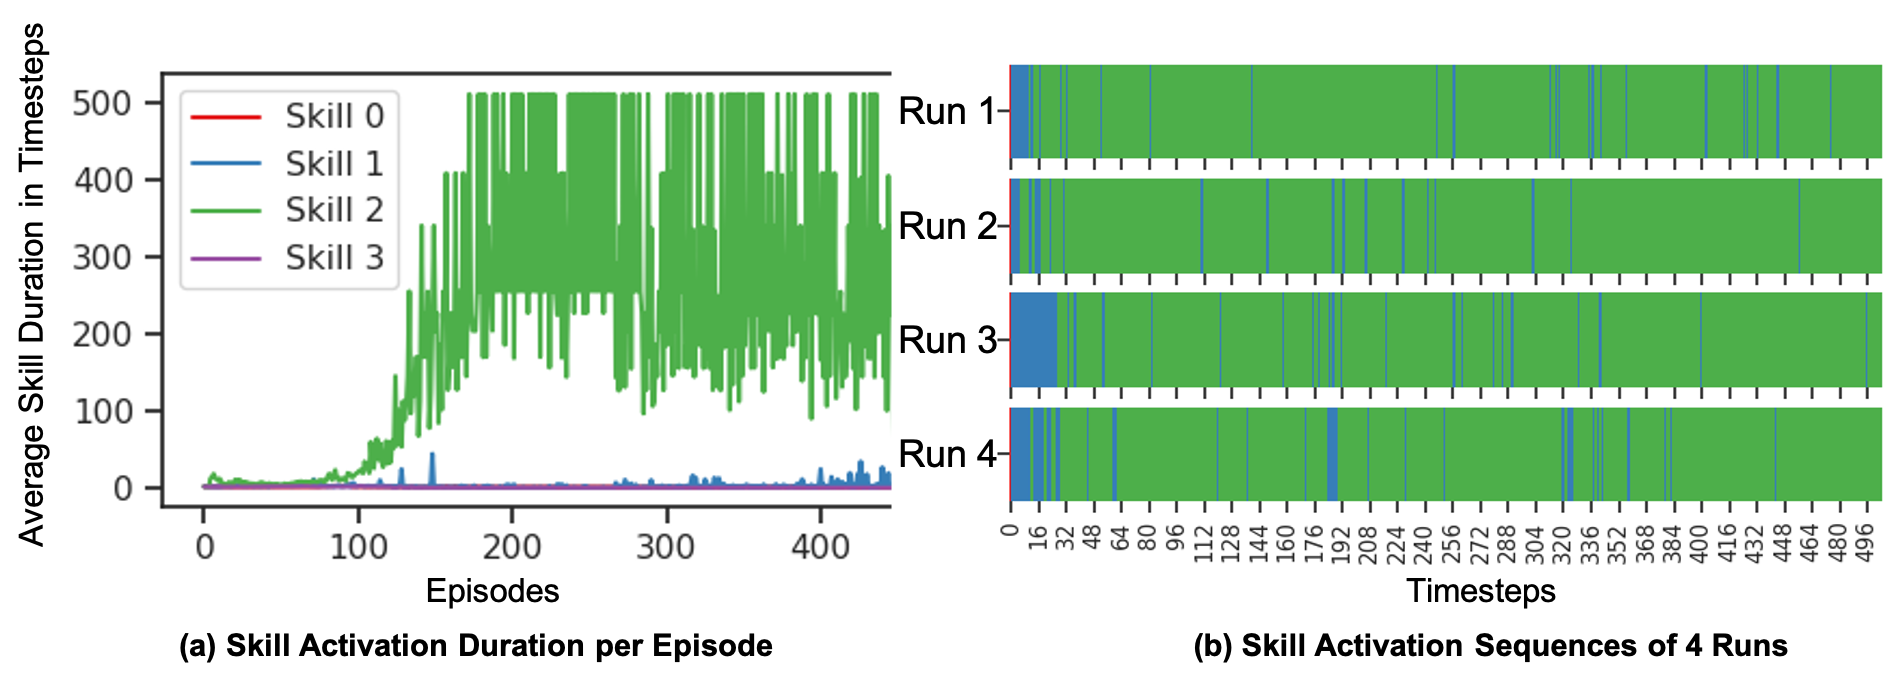
\includegraphics[width=0.7\linewidth]{./Part1/figures/skill_sequence_joint.png}\\
  \vspace{-4mm}\caption{\label{fig:skill_sequence} Skill Duration
  Patterns}\vspace{-3mm}
\end{figure*}
\begin{figure*}[h]
  \centering
  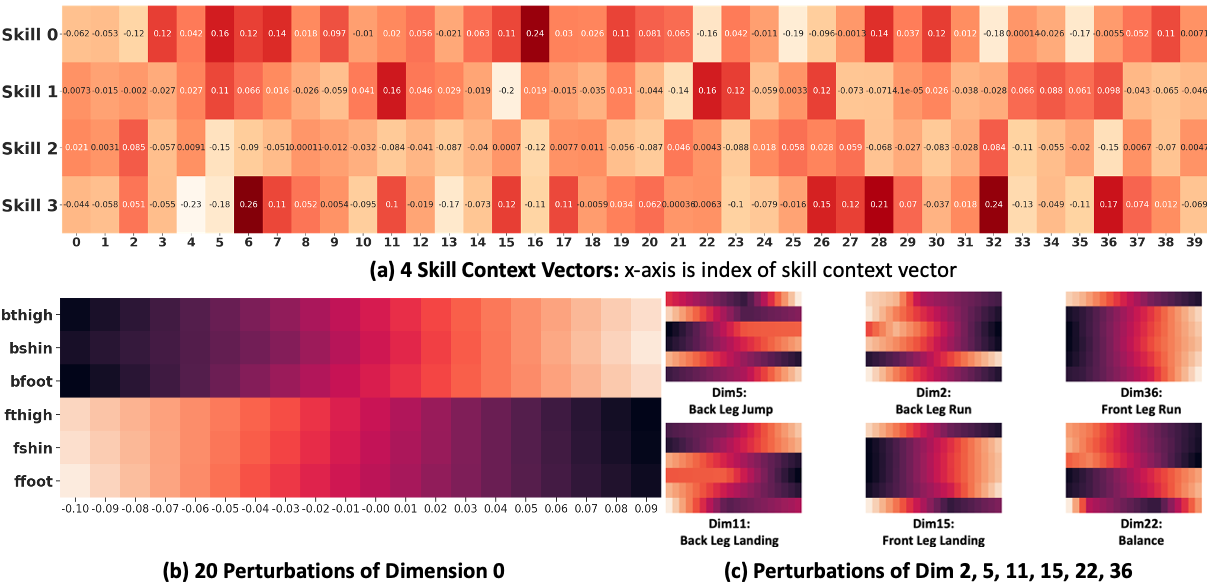
\includegraphics[width=0.75\linewidth]{./Part1/figures/Interp_joint.png}\\
  \vspace{-4mm}\caption{\label{fig:interp_joint} Interpretation
    of Skill Context Vectors}\vspace{-4mm}
\end{figure*}

% to write: in this section,
In this section, we design experiments to answer three questions:
1) Can SA outperform other baselines (regarding episodic returns,
stability, and scalability)? 2) Can SA temporally extend skills
without the termination function? 3) Can skill context vectors be
easily interpreted? 4) Does skill embeddings learned by SA have a
performance boost over other option variants in transfer learning
settings?

For single task learning, experiments are conducted on all OpenAI
Gym MuJoCo environments (10 environments)
\cite{brockman2016openai}. We follow DAC~\cite{zhang2019dac} and
compare our algorithm with five baselines, four of which are
option implementations, i.e., DAC+PPO \cite{zhang2019dac},
AHP+PPO \cite{levy2011unified}, PPOC
\cite{klissarov2017learnings} and OC \cite{bacon2017option}. The
last baseline is PPO \cite{schulman2017proximal}. All baselines'
parameters used in DAC\footnote{All baselines' implementations
  are from DAC's open source repo
  https://github.com/ShangtongZhang/DeepRL/tree/DAC. Note that
  the author list of this paper does not have any overlap with
  DAC. Our source code is available in supplementary materials.}
remain unchanged other than the maximum number of training steps:
SA only needs 1 million steps to converge rather than the 2
million used in DAC. For transfer learning, we follow
\citename{zhang2019dac} and run 6 pairs of transfer learning
tasks constructed in DAC based on DeepMind Control Suite
\cite{tassa2020dmcontrol}. For a fair comparison, we use four
skills for SA and four options for other option implementations.
All experiments are run on an Intel® Core™ i9-9900X CPU @ 3.50GHz
with a single thread and process. Our implementation details are
summarized in Appendix~\ref{sec:append_implement}.

\begin{figure*}[h]
  \vspace{-2mm}
  \centering
  \includegraphics[width=1\linewidth]{./Part1/figures/transfer.png}\\
  \vspace{-4mm}
  \caption{\label{fig:transfer} Performance on DAC transfer
    learning tasks}
  \vspace{-4mm}
\end{figure*}

\subsection{Single Task Learning}
\label{sec:exp_perf}
\vspace{-2mm}
% towrite: figure capitalize
In Figure~\ref{fig:exp_dac}, we report episodic returns on
infinite horizon and finite horizon\footnote{We refer to
  environments with the game-over condition as finite horizon
  environments, and infinite vice versa.} environments
separately. For a fair comparison, we use exactly the same
plotting script as used in DAC: curves are averaged over 10
independent runs and smoothed by a sliding window of size 20.
Shaded regions indicate standard deviations. Performance of all
ten environments is shown in (Appendix
Figure~\ref{fig:all_tasks}, Table~\ref{table:single_infinite}).

It is extremely interesting that SA shows two completely
different kinds of behaviors on infinite and finite horizon
environments. According to previous option framework
implementations~\cite{klissarov2017learnings,smith2018inference,harb2018waiting,zhang2019dac},
on single task environments, option-based algorithms do not have
a distinguishable performance boost over hierarchy-free
algorithms. SA also has similar behavior and achieves comparable
performance to the best baseline algorithm on most finite horizon
environments (Figure~\ref{fig:exp_dac} (b)). In
Appendix~\ref{sec:append_gist} we conceptually explain that
conventional value functions are insufficient to approximate
models which have temporal latent variables dependencies. A
concrete deep wide skill-action architecture remains open for the
future work.

On infinite horizon environments as shown in
Figure~\ref{fig:exp_dac} (a), SA's performance significantly
outperforms all baselines by a large margin in various aspects.
For episodic return, e.g., HumanoidStandup, all option
implementations barely converge, while SA is $240\%$ better than
DAC and AHP\footnote{Even on Reacher, a simple environment on
  which most algorithms converge to a similar performance, SA is
  still $38\%$ better than the second best (AHP).}. For
convergence, SA has the fastest convergence speed. On the first
two environments, which are also reported in DAC, SA only takes
$40\%$ of time steps of DAC and AHP to reach similar episodic
returns. This acceleration is because: 1) SA is MDP formulated,
the skill policy is updated at each time step; 2) SA only has one
action policy decoder; 3) the action decoder learns to decode
skill context vectors whichever skill is activated. For
stability, all 10 runs of SA converge to a similar level while
the other have much larger standard deviations. This property is
theoretically justified by Proposition~\ref{prop:var_red} and
further discussed in Appendix~\ref{sec:append_gist}.

\vspace{-2mm}
\subsection{Temporal Extension}
\label{sec:exp_ext}

It is logical to ask whether SA is capable of temporal extension
without the termination function. To illustrate this, we plot the
average duration of each skill during training episodes of the
HalfCheetah environment in Figure~\ref{fig:skill_sequence} (a)
and 4 runs of skill activation sequences in
Figure~\ref{fig:skill_sequence} (b). (more details in
Appendix~\ref{sec:append_exp_ext}). At the start of training, all
skills' durations are short, while Skill 2's duration quickly
grows and dominates the entire episode. This growth of duration
proves that SA can still temporally extend a skill. Towards the
end of the training, the dominant skill's duration starts to
decrease while the duration of a secondary skill (Skill 1) starts
to increase. This means that during later training stages, SA
starts to coordinate different skills. The dominant skill
phenomenon is also reported in other option implementations such
as DAC. However, as shown in the
video\footnote{https://www.youtube.com/watch?v=QiLVZvI6NJU}, SA
still learns distinguishable skills. Skill 2 is the running
forward skill thus it dominates the whole episode. Skill 1 is
only used to recover from falling down thus it has much shorter
duration. As discussed in Appendix \ref{sec:append_gist},
solution to the dominant skill is actually learning skills at
much finer granularity. The SA-style wide value function
(Eq.~(\ref{eq:sa_v})) provides an elegant solution to this
problem.

\vspace{-2mm}
\subsection{Interpretation of Skill Context Vectors}
\label{sec:interpret}

Explicit skill representations not only improve efficiency,
scalability, and generalization, but also benefit interpretation.
We continue with the HalfCheetah example and demonstrate how
easily skill context matrix $\mW_s$
(Figure~\ref{fig:interp_joint} (a)) can be interpreted (more
details are provided in Appendix~\ref{sec:append_interpret}). We
first follow \citename{sabour2017dynamic} and interpret what
property is represented by a context vector's dimension by adding
perturbations on to it, and inspecting perturbations' effects
on the action policy decoder in generating primary actions $\rva$
(Figure~\ref{fig:interp_joint} (b)). Once each dimension is
understood, skills become straight forward to interpret by simply
inspecting on which dimensions (property) each skill $\hat{\rvo}$
in Figure ~\ref{fig:interp_joint} (a) has significant weights,
and interpreting properties of those dimensions
((Figure~\ref{fig:interp_joint} (c)). In this way, we can
interpret that Skill 2 is a forward movement skill, since it
focuses on jumping and running forward, while Skill 1 is a
landing skill. These interpretations can further be used to
explain skill activation patterns in
Figure~\ref{fig:skill_sequence} (b): Skill 2 has the longest
duration because it is the major source of all forward movements.
Skill 2 occasionally falls back to Skill 1 because, after jumping
or running, the HalfCheetah needs to land and balance itself.


\subsection{Transfer Learning}
\label{sec:transfer}

We follow \citename{zhang2019dac} and run 6 pairs of transfer
learning tasks constructed in DAC based on DeepMind Control Suite
\cite{tassa2020dmcontrol}. Each pair contains two different
tasks. To keep consistent with DAC, we train all models one
million steps on the first task and switch to the second (SA's
skill context matrix is subsequently frozen) to run another one
million steps. Results are reported in Figure~\ref{fig:transfer}
(Appendix Table~\ref{table:transfer}). On the first task, SA's
performance is among the best algorithms in all environments.
This further validates SA's advantages on single task as observed
in section~\ref{sec:exp_perf}. On the transfer learning (the
second) task, SA's performance ranks the first in 5 out of 6
environments. This shows SA's advantages in knowledge reuse
tasks. \vspace{-2mm}

\section{Conclusions}
\label{sec:conclusion}
\vspace{-2mm}

In this paper, we presented a novel MDP equivalence of the SMDP
formulated option framework, from which an MDP implementation of
the option framework, i.e., the Skill-Action architecture, was
derived. We theoretically proved that SA has lower variance than
conventional RL models and provided policy gradient theorems for
updating SA. Our empirical studies on challenging infinite
horizon robot simulation environments demonstrated that SA not
only outperforms all baselines by a large margin, but also
exhibits smaller variance, faster convergence, and good
interpretability. On transfer learning, SA also outperforms the
other models in 5 out of 6 environments and shows its advantages
in knowledge reuse tasks.

The final and most important contribution of SA is hierarchically
learning explicit abstract actions' representations with ``skill
context vectors''. This design significantly improves the
scalability and interpretability of SA. It is straightforward to
extend SA to deeper and wider (Appendix~\ref{sec:append_gist})
architectures, which gives rise to a large-scale pre-training and
transfer learning architecture in the reinforcement learning
area.

Experiments also show that SA shares two innate limitations with
the conventional option framework
\cite{levy2011unified,klissarov2017learnings,smith2018inference,harb2018waiting,zhang2019dac}:
(1) failure to improve the performance and the sample efficiency
on finite horizon environments (section~\ref{sec:exp_perf}); (2)
``the dominant skill problem'' \cite{zhang2019dac} (section
\ref{sec:exp_ext}). In Appendix~\ref{sec:append_gist} we
conceptually discuss that SA-style wide (higher-order
dependencies) value functions could be a solution to both
limitations. This is mainly because these limitations are caused
by the insufficiency of the conventional value functions in
approximating values that have temporal latent variables
dependencies (discussed in Appendix~\ref{sec:append_gist}).



%%% Local Variables:
%%% mode: latex
%%% TeX-master: "../thesis"
%%% End:


\part{Undirected Probabilistic Graphical Model: Markov Random
  Fields}
\label{part:2}
%% 
%% 
%% 

\chapter{Modeling Higer-order Structural Dependencies with Markov Random Fields (MRFs)}
\chaptermark{MRF-LSSVMs}
\label{cha:mrf}

One challenging task in machine learning is recognizing and
labeling over complex and structured objects. Many applications,
such as image segmentation, motif finding and noun-phrase
parsing, involves representing jointly correlated sub-objects and
exploiting structural dependencies to identify higher level
objects. These objects usually have structural dependencies on
sub-objects (smaller components), \eg the human face has a strong
structural dependency on five sensory organs. The Markov Random
Fields (MRFs, are also called undirected Probabilistic Graphical
Models~\cite{bishop:2006:PRML}), is one of the most popular
framework in modeling structural dependencies. In this Chapter,
we propose novel exact inference and learning algorithms, the
MRF-LSSVMs (Latent Structural Support Vector Machine) framework,
to exploit MRFs' capabilities in modeling higher-order (more than
three entities) structural dependencies. The application of
MRF-LSSVMs to capture higher-order dynamics on time series is
discussed in \Chapref{cha:mrf_lssvm_app}.

Markov Random Fields (MRFs) are undirected Probabilistic
Graphical Models (PGMs). The formulation of MRFs is simply a
regularized joint probability distribution. One specialty of MRFs
is that they are factorized (conditional independent) over
\textbf{maximal cliques} (more details in~\Secref{sec:MRF}) of
random variables defined on the undirected
graph~\cite{bishop:2006:PRML}. In many applications, structural
information, such as sub-objects to the whole object
relationships and relationships between sub-objects, can be well
represented in maximal cliques. By defining each maximal clique's
probability distribution and optimizing over them, MRFs provide a
powerful framework for modeling complex higher-order
dependencies between entities.

Utilizing MRFs usually involves three steps: 1) designing energy
functions (un-normalized probability distribution) according to
the actual problem, 2) solving inference problem (MAP or energy
minimization), and 3) learning parameters from data set. With
respect to energy functions, our work focuses on Lower Linear
Envelope Potentials (LLEP), a class of higher-order potentials
defined as a concave piecewise linear function over a clique of
random variables. LLEP has been raising much interest in the
image segmentation area, in which the raw image input is used as
PGM's graph and pixels are treated as random variables. Maximal
cliques of the input image are usually detected at preprocessing
stage by using clustering algorithms such as
superpixel~\cite{achanta2012slic}. Success of LLEP on encoding
consistent constraints over large subsets of pixels in image
segmentation tasks has been witnessed in many
literatures~\cite{Kohli:CVPR07,Nowozin:2011, Song2015}. In this
chapter we focus on proposing a novel exact inference algorithm
for LLEP and design a learning algorithm under the LLSVM
framework. In \Chapref{cha:mrf_lssvm_app}, we will generalize the
MRF-LLSVMs framework into encoding consistent constraints among
time-series' entities.

In the second step, in order to solve the inference problem of
LLEP, \citename{kohli2009robust} proposed a method to represent a
class of higher order potentials with lower (upper) linear
envelope potentials. By introducing auxiliary
variables~\cite{Kohli:CVPR10}, they reduced the linear
representation to a pairwise form and proposed an approximate
algorithm with standard linear programming methods. However, they
only show an exact inference algorithm on at most three terms.
Following their approach, \citename{gouldlearning} extended their
method to a weighted lower linear envelope with arbitrary many
terms solved with an efficient algorithm. They showed that the by
introducing auxiliary variables into LLEP, a quadratic
pseudo-Boolean form~\cite{Boros:MATH02} can be developed. This
psuedo-Boolean form is submodular and can be inferred efficiently
and exactly through graph-cuts like
algorithms~\cite{Boykov:ICCV01}. However, in order to employ
Structural Support Vector Machine (SSVM) to solve the learning
problem of LLEP, \citename{gouldlearning} have to sample the LLEP
using a set of fixed space points. Althought this formulation can
be globally optimized by using the SSVM framework, it lost a rich
class of representations of energy function due to the fixed
space sampling. In this chapter, we an alternative formulation to
learn LLEP exactly. We introduce auxiliary variables back to LLEP
and propose a graph-cuts algorithm to infer observed variables
and auxiliary variables simultaneously. Experiments in
~\Secref{sec:synth-check} also show that LLEP under this
formulation the algorithm can be learned exactly from various
different probability distribution configurations.

The third and last difficulty is to design a learning algorithm
for our LLEP formulation. In previous work,
\citename{gouldlearning} sampled the LLEP with fixed space points
and solved the learning problem under the Structural Support
Vector Machine (SSVM) framework \cite{tsochantaridis2005large}.
However, since we add auxiliary variables back, SSVM does not fit
our case anymore. One of our main contribution is that we prove
that auxiliary variables introduced in LLEP can be formulated as
latent variables in SSVM. With additional convex constraints
added to the SSVM object, our formulation results to the Latent
SSVM (LSSVM) framework \cite{yu2009learning}. The LSSVM was
developed by \citename{felzenszwalb2008discriminatively} and
\citename{yu2009learning} independently in different ways. The
main idea is introducing a latent variable to extend the feature
vector, which results in an arbitrary loss function, e.g. Hinge
Loss, with an upper bound. Then the optimization was done by
using Concave-Convex Procedure (CCCP) algorithm, which is
guaranteed to decrease the objective function to a local minimum.
In this thesis, we propose a variant formulation of
\cite{gouldlearning} by rewriting the lower linear envelope
function directly into a linear combination with latent feature
vectors and developing the learning algorithm using the LSSVM.

The rest of the thesis is structured as follows:
\Secref{sec:RelatedWorks} introduces background and related works
of MRFs and LSSVM. \Secref{sec:inference} proposes our first
contribution, the exact inference method of LLEP with auxiliary
variables. In~\Secref{sec:learning}, we reformulate the LLEP into
a linear combination and develop the learning algorithm under the
LSSVM framework. \Secref{sec:synth-check} conduct experiments on
a synthetic checkerboard image to show the effectiveness of our
novel MRF-LLSVMs framework. Application of MRF-LLSVMs on real
financial time-series data set is discussed in
\Chapref{cha:mrf_lssvm_app}.

\section{Background \& Related Works}
\label{sec:RelatedWorks}

\subsection{Markov Random Fields}
\label{sec:MRF}
From a PGMs view (\figref{fig:prml_mrf}) \cite{Bishop:2007},
MRFs' joint probability distribution can be represented as an
undirected graph and each random variable can be represented as a
node in the graph. A \textbf{clique} is a fully connected subset
of nodes: there exists a path between any pair of nodes in it. A
\textbf{maximal clique} is a clique such that it is not possible
to include any other nodes from the graph in the set without it
ceasing to be a clique.
\begin{figure}[ht]
  \centering
  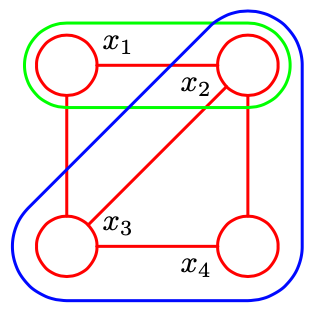
\includegraphics[width=0.3\columnwidth]{Part2/figures/prml_mrf}
  \caption{\label{fig:prml_mrf} An example PGM of MRFs. Each node
    in this graph corresponds to a random variable in this PGM's
    joint probability distribution. A clique is outlined in green
    circle and a maximal clique is outlined in blue circle.}
\end{figure}
Let $C$ denotes a maximal clique in one graph and $\vy_C$ denotes
the set of variables in that clique. Then the joint distribution
can be written as:
\begin{align}
  p(\vy)=\frac{1}{Z}\prod_{C}{\Psi_C(\vy_C)}
\end{align}
\noindent where $\Psi$ is called \emph{potential functions} which
can be defined as any non-negative functions and
$Z=\sum_{\vy}\prod_{C}{\Psi_C(\vy_C)}$ which is a normalization
constant. To infer labels which best explains input data set, we
can find the \emph{maximum a posteriori} (MAP) labels by solving
$\vy^*=\argmax_{\vy}p(\vy)$. However, potential functions are
restricted to be non-negative to ensure it is a probability
distribution.

In order to have more flexible representations of probability
distributions, by taking exponential of potential terms, MRFs can
be represented as a regularized joint log-probability
distribution of arbitrary non-negative functions over a set of
maximal cliques on the PGM graph~\cite{bishop:2006:PRML}. Thus
the joint distribution becomes:
\begin{align}
  p(\vy)=\frac{1}{Z}exp(-\sum_{C}{E_C(\vy_C)})
\end{align}
\noindent where $E$ is called \emph{energy functions} which can be
arbitrary functions. Therefore, \emph{maximum a posteriori}
problem is equivalent to \emph{energy minimization} problem,
which is also known as the \emph{inference} problem:
\begin{align}
  \vy^*=\argmax_{\vy}p(\vy)=\argmin_{\vy}(\sum_{C}{E_C(\vy_C)})
\end{align}

The \emph{inference} problem is computationally expensive. There
has been many sub-optimal algorithms such as max-product
algorithm \cite{Globerson:NIPS07} been proposed to solve the
general MRFs' inference problem. However, \citename{Boros:MATH02}
proved that for submodular energy functions, there exist
efficient algorithms based on graph cuts
\cite{Ishikawa:CVPR09,Kohli:TR08} and are guaranteed to converge
to the global optimum. In \Secref{sec:inference} we formulate the
MRFs with Lower Linear Envelope Potentials (LLEP) as
psuedo-boolean functions and devise a graph cut algorithm for
exact inference.

As for the \emph{learning} problem, conventionally, energy
functions can be decomposed into three weighted parts: nodes
$\gN$, edges $\gE$ and higher order cliques (any group which has
more than 3 fully connected nodes in it)
$\gC$~\cite{Szummer:ECCV08}. Each term has its own weights. Let
$\vw$ be the vector of parameters and $\phi$ be arbitrary feature
function, then the energy can be decomposed as a set linear
combinations of weights and feature vectors:

\begin{align}
  \label{eq:energyfunction_UPH}
  E(\vy;\vw)=\sum_{i\in \gN}{\vw_i^U\phi^U(\vy_i)}+
  \sum_{(i,j)\in \gE}{\vw_{ij}^P\phi^P(\vy_i,\vy_j)}+
  \sum_{\vy_C\in \gC}{\vw_C^H\phi^H(\vy_C)}
\end{align}

\noindent where $U$ denotes \emph{unary} terms, $P$ denotes
\emph{pairwise} terms and $H$ denotes \emph{higher order} terms
(when $|C|>2$ namely each clique contains more than two
variables).

A weight vector $\vw$ is more preferable if it gives the
ground-truth assignments $\vy_t$ less than or equal to energy
value than any other assignments $y$:

\begin{align}
E(y_t,w)\leq E(y,w)~ \text{,~}\forall y \neq y_t
\text{,~} y\in \sY
\end{align}

Thus the goal of \emph{learning} MRFs is to learn the parameter
vector $\vw^*$ which returns the lowest energy value for the
ground-truth labels $y_t$ relative to any other assignments
$y$~\cite{Szummer:ECCV08}:

\begin{align}
\vw^* = argmax_{\vw}(E(y_t,w)-E(y,w))~ \text{,~}\forall y \neq y_t
\text{,~} y\in \sY
\end{align}

Solving the learning problem of MRFs is also computationally
expensive. In this thesis, we employ the efficient Latent
Structural Support Vector Machines (LSSVMs) algorithm to solve
our MRFs.

\subsection{Latent Structural SVMs}
\label{sec:latent-struct-svms}

The Structural Support Vector Machines (SSVMs) (also called
max-margin
framework)~\cite{Taskar:ICML05,tsochantaridis2005large} is a
principled approach to learn weights of pairwise MRFs
\citename{Szummer:ECCV08,Gould:ICML2011}.
\citename{gouldlearning} extended this framework with additional
linear constraints to enforce concavity on the weights, thus
allowing them to be used to learn MRFs with lower linear envelope
potentials. However, because SSVM does not include latent
variables in its feature vector, such methods only approximately
learn higher-order functions. In this thesis, we propose an
algorithm to optimize the energy function exactly by introducing
auxiliary variables back into the feature vector and solving the
learning problem using the Latent Structural SVMs (LSSVMs)
framework~\cite{yu2009learning}. To include unobserved
information, \citename{yu2009learning} extended the joint feature
function in structural SVM with latent variables and re-wrote the
objective function of SSVM into a difference of two convex
functions. This formulation can be solved using the
Concave-Convex Procedure (CCCP)\cite{yuille2002concave} which is
two-stages algorithm that guarantee to convergence to a local
minimum.

Specifically, given an a linear combination of features vector
$\phi(\vx ,\vy) \in \sR^m$ and weights $\vtheta \in \sR^m$, and a
set of $n$ training examples $\{\vy_i\}_{i=1}^n$ max-margin
framework can be used to solve optimized solution $\vtheta^*$. To
include unobserved information in the model,
Yu\cite{yu2009learning} extended the joint feature
function\cite{tsochantaridis2005large} $\phi(\vx,\vy) $ with a
latent variable $\vh\in \mathcal{H}$ to $\phi(\vx,\vy,\vh) $. So
the inference problem becomes
\begin{align}
  \label{eq:latent_ssvm_linearcomb}
  f_\theta(x) = \argmax_{(\vy \times \vh) \in \sY
  \times \sH} \vtheta\cdot\phi(\vx,\vy,\vh)
\end{align}

Accordingly, the loss function can be extended as

$$
\Delta((\vy_i,\vh^*_i(\theta)),(\hat{\vy}_i(\vtheta),\hat{\vh}_i(\vtheta)))
$$

\noindent where

\begin{align}
  \label{eq:latentssvm_full_inf}
 (\hat{\vy}_i(\vtheta),\hat{\vh}_i(\vtheta))=\argmax_{(\vy
  \times \vh) \in \mathcal{Y} \times \mathcal{H}}
\theta\cdot\phi(\vx_i,\vy,\vh)
\end{align}

\begin{align}
  \label{eq:latentssvm_latent_inf}
  \vh^*_i(\theta) = \argmax_{\vh \in \mathcal{H}} \theta \cdot
  \phi(\vx_i,\vy_i,\vh)
\end{align}

The loss function under this formulation measures difference
between the inferred result pair $(\hat{\vy}_i(\theta),
\hat{\vh}_i(\theta))$ and the pair $(\vy_i(\theta),
\vh_i^*(\theta))$ which best explains the training data. However,
under this formulation the ``loss augmented inference'' used in
structural SVMs\cite{tsochantaridis2005large} to remove the
complexity cannot be performed due to the dependence of loss
function $\Delta$ on hidden variables $\vh^*_i(\theta)$.
\citename{yu2009learning} argued that in real world applications
hidden variables are usually intermediate results and are not
required as an output\cite{yu2009learning}. Therefore, the loss
function can only focus on the inferenced hidden variables
$\hat{\vh}_i(\theta)$ which leads to:

$$
\Delta((\vy_i,\vh^*_i(\theta)),(\hat{\vy}_i(\theta),\hat{\vh}_i(\theta)))
=
\Delta(\vy_i,\hat{\vy}_i(\theta),\hat{\vh}_i(\theta))
$$

Thus the upper bound used in standard structural
SVMs\cite{tsochantaridis2005large} can be extended to:

\begin{align}
  \nonumber\Delta((\vy_i,\vh^*_i(\theta)),(\hat{\vy}_i(\theta),\hat{\vh}_i(\theta)))
  &\leq \bigg(\max_{(\hat{\vy} \times \hat{\vh}) \in
    \mathcal{Y} \times \mathcal{H}}
    [\theta\cdot\Psi(\vx_i,\hat{\vy},\hat{\vh}) +
    \Delta(\vy_i,\hat{\vy},\hat{\vh})]\bigg)\\
  &-\max_{\vh \in \mathcal{H}} \theta \cdot
    \Psi(\vx_i,\vy_i,\vh)
\end{align}

Hence the optimization problem for Structural SVMs with latent
variables becomes

\begin{align}
\label{eq:latent_ssvm_object}
  \min_\theta\bigg(\frac{1}{2}\|\theta\|^2+
  C\sum_{i=1}^{n}\big(\max_{(\hat{\vy} \times
  \hat{\vh}) \in \mathcal{Y} \times \mathcal{H}}
  [\theta\cdot\Psi(\vx_i,\hat{\vy},\hat{\vh}) +
  \Delta(\vy_i,\hat{\vy},\hat{\vh})]\big)\bigg)\\
  -C\sum_{i=1}^{n}\big(\max_{\vh \in \mathcal{H}} \theta \cdot
  \Psi(\vx_i,\vy_i,\vh)\big)\nonumber
\end{align}

\noindent which is a difference of two convex functions. Problem
of this formulation can be solved using the Concave-Convex
Procedure (CCCP)\cite{yuille2002concave} which is guaranteed to
converge to a local minimum. \citename{yu2009learning} proposed a
two stages algorithm. In the first step the latent variable
$\vh_i^*$ which best explains training pair $(\vx_i, \vy_i)$ is
found by solving equation~\eqref{eq:latentssvm_latent_inf}. This
step is also called the ``latent variable completion'' problem.
In the second step $\vh_i^*$ is used as completely observed to
substitute $\vh$ in equation~\eqref{eq:latent_ssvm_object}.
Therefore, solving equation~\eqref{eq:latent_ssvm_object} is
equivalent to solve the standard structural SVM problem.

In contrast to SVM, the latent structural SVM only provides an
optimization framework and cannot be directly applied. In order
to use it, the inference algorithm, as well as the MRF feature
function, loss function, and latent variable completion
problem~\cite{yu2009learning} must first be specified. Our
implementation of these terms are described in
section~\ref{sec:opt}.

\section[MRFs with LLEPs]{Markov Random Fields (MRFs) with Lower
  Linear Envelope Potentials (LLEPs)}
\label{sec:inference}

Energy functions can be decomposed over nodes $\gN$, edges $\gE$
and higher order cliques $\cal C$~\cite{Szummer:ECCV08}. Let
$\vw$ be vector of parameters and $\psi$ be arbitrary feature
function, then the energy can be decomposed as a set of linear
combinations of weights and feature vectors:

\begin{align}
  \label{eq:energyfunction_UPH}
  E(\vy;\vw)&=\sum_{i\in \gN}{\vw_i^U\psi^U(\vy_i)}+ \notag\\
  & \sum_{(i,j)\in \gE}{\vw_{ij}^P\psi^P(\vy_i,\vy_j)}+
  \sum_{\vy_C\in \cal C}{\vw_C^H\psi^H(\vy_C)}
\end{align}

\noindent where $U$ denotes \emph{unary} terms, $P$ denotes
\emph{pairwise} terms, $H$ denotes \emph{higher order} terms. In
this section we mainly focus on one class of higher-order
potentials $\psi^H$ defined as a concave piecewise linear
function which is known as \emph{Lower Linear Envelope
  Potentials} (LLEP). 

LLEP has been studied extensively in Markov Random Fields area
for encouraging consistency over large
cliques~\cite{Kohli:CVPR07,Nowozin:2011,Gould:ICML2011}. In
\Secref{sec:llep}, we begin with developing standard Markov
Random Fields (MRFs) (equation~\eqref{eq:energyfunction_UPH})
with the LLEP as energy functions. We then show how to perform
exact inference under this formulation in
\Secref{sec:exact_inference}. The optimization algorithm for our
formulation will be discussed in \Secref{sec:learning}.

\subsection{Higher-order Energy Functions: Weighted Lower Linear
  Envelope Potentials (LLEP)}
\label{sec:llep}

Let $\cal C$ denotes the set of all maximal cliques
and $\vy_c=\{y_i |\text{\,for\,} i \in C_j\}$ denotes set of
binary random variables where $y_i\in \{0,1\}$ in clique $C_j$, a
weighted lower linear envelope potential over $\vy_c$ is defined
as the minimum over a set of $K$ linear functions as:
%
\begin{align}
  \psi^H_c\!(\vy_c) \, &= \min_{k=1, \ldots, K} \left\{ a_k W_{\!c}(\vy_c) + b_k \right\}.
  \label{eqn:potential2}
\end{align}
%
where $W_{\!c}(\vy_c) = \sum_{i \in c} w_i^c y_i$ with $w^c_i
\geq 0$ and $\sum_{i \in c} w^c_i = 1$ which are weights for each
clique. $(a_k, b_k) \in \sR^2$ are the linear function
parameters. We illustrate an example with four linear functions
in \figref{fig:concave}.

\begin{figure}[t]
  \centering
  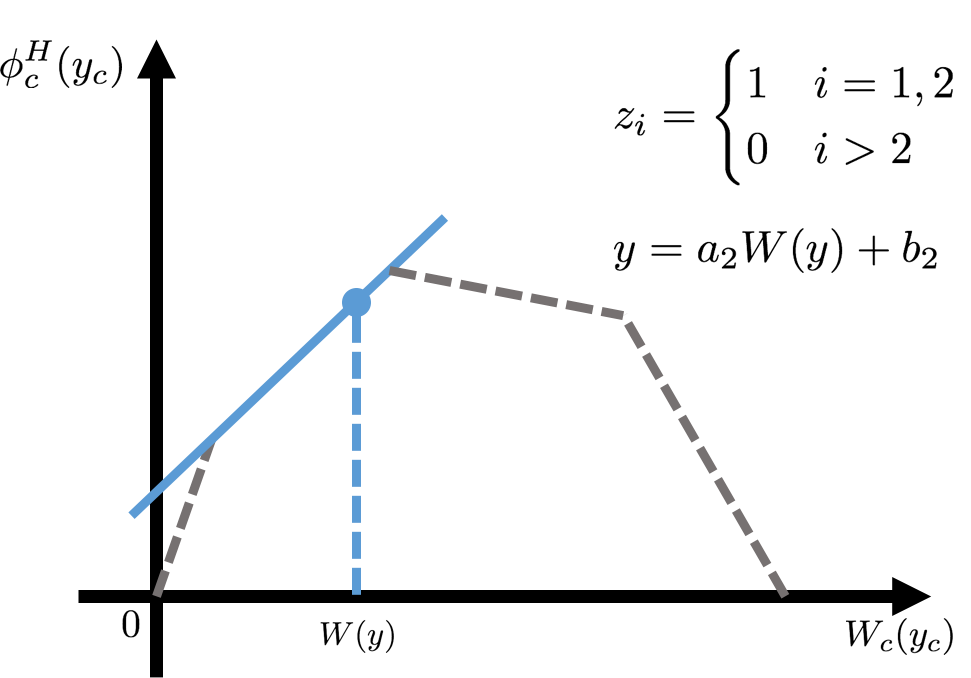
\includegraphics[width=0.8\columnwidth]{Part2/figures/linEnvLatentFig.png}
  \caption{\label{fig:concave} Example piecewise-linear concave
    function of $W_{\!c}(\vy_c) = \sum_{i \in c} w^c_i y_i$.
    Assume the second linear function is active namely
    $\vz^c=(1,1,0,0)$ (equation \ref{eqn:binary_concave_z}). The result of linear combination of
    parameter vector and feature vector is same as quadratic
    pseudo-Boolean function.}
\end{figure}

% % to_replace
% \begin{figure}[ht]
%   \centering
%   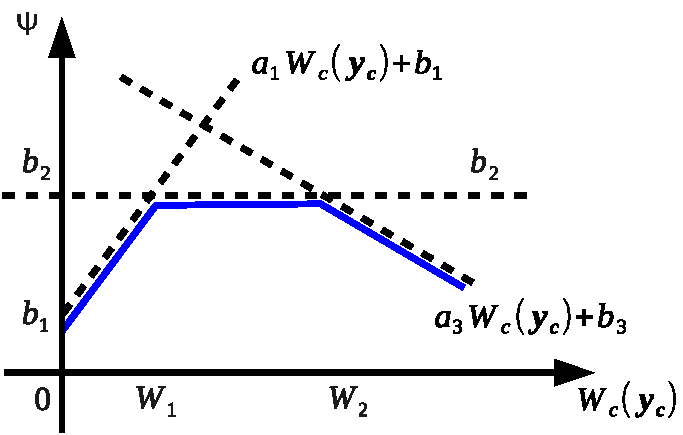
\includegraphics[width=0.6\columnwidth]{Part2/figures/not_redundant}
%   \caption{\label{fig:nonredundant} Example lower linear envelope
%     $\psi^H_c\!(\by_c)$ (shown solid) with three terms (dashed).
%     When $W_{\!c}(\by_c) \leq W_1$ the first linear function is
%     active, when $W_1 < W_{\!c}(\by_c) \leq W_2$ the second
%     linear function is active, otherwise the third linear
%     function is active.}
% \end{figure}

Inference on energy function contains lower linear potentials is
the same as the standard equation~\eqref{eq:energyfunction_UPH}
and is given by:
\begin{align}
  \label{eq:min_energy}
  \vy^* = \argmin\energy{\vy}
\end{align}

Suppose that parameters $\{(a_k, b_k)\}_{k=1}^K$ are sorted in
decreasing order of $a_k$. From \emph{Definition 3.1}
\cite{gouldlearning} we know that the $k$-th linear function is
said to be \emph{active} if there exists $x \in (0, 1)$ such that
the following two inequalities hold
\begin{align}
  a_{k-1} x + b_{k-1} &> a_k x + b_k \nonumber \\
  a_{k+1} x + b_{k+1} &> a_k x + b_k
  \label{eqn:nonred_in_ab}
\end{align}
%
The $k$-th linear function is said to be \emph{redundant}
(\emph{Definition 3.2}~\cite{gouldlearning}) if it is not active
for any assignment to $\vy_c$ in any clique $c \in \gC$ or is only
active whenever another linear function is also active.
Figure \ref{fig:redundant} depicts such conditions. As a
result, removing redundant functions from the potential does not
chang the energy function.


From section~\ref{sec:MRF} we have already introduced that an
\emph{energy function} may contain \emph{unary}, \emph{pairwise}
and \emph{higher-order} potentials (see
equation~\eqref{eq:energyfunction_UPH}). In this section we
mainly focus on one class of higher-order potentials $\phi^H$
defined as a concave piecewise linear function which is known as
\emph{lower linear envelope potentials}. This has been studied
extensively in Markov Random Fields area for encouraging
consistency over large
cliques~\cite{Kohli:CVPR07,Nowozin:2011,Gould:ICML2011}.

Let $\gC$ denotes the set of all maximal cliques in an image and
$\vy_c=\{y_i |\text{\,for\,} i \in c\}$ denotes set of random
variables in the clique $c$, a weighted lower linear envelope
potential~\cite{gouldlearning} over $\vy_c$ is defined as the
minimum over a set of $K$ linear functions as:
%
\begin{align}
  \psi^H_c\!(\vy_c) \, &= \min_{k=1, \ldots, K} \left\{ a_k W_{\!c}(\vy_c) + b_k \right\}.
  \label{eqn:potential2}
\end{align}
%
where $W_{\!c}(\vy_c) = \sum_{i \in c} w_i y_i$ with $w^c_i \geq
0$ and $\sum_{i \in c} w^c_i = 1$ which are weights for each
clique. $(a_k, b_k) \in \sR^2$ are the linear function
parameters. We illustrate an example~\cite{gouldlearning} with
three linear functions in \figref{fig:nonredundant}.
%
\begin{figure}[ht]
  \centering
  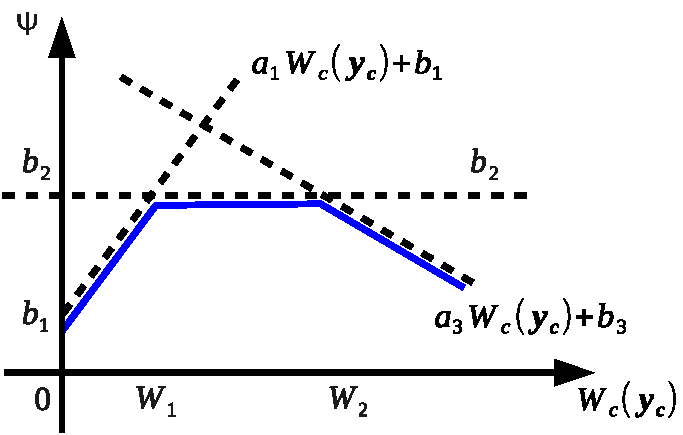
\includegraphics[width=0.6\columnwidth]{Part2/figures/not_redundant}
  \caption{\label{fig:nonredundant} Example lower linear envelope
    $\psi^H_c\!(\vy_c)$ (shown solid) with three terms (dashed).
    When $W_{\!c}(\vy_c) \leq W_1$ the first linear function is
    active, when $W_1 < W_{\!c}(\vy_c) \leq W_2$ the second
    linear function is active, otherwise the third linear
    function is active.}
\end{figure}

Suppose that parameters $\{(a_k, b_k)\}_{k=1}^K$ are sorted in
decreasing order of $a_k$. \citename{gouldlearning} (Definition
3.1) defines that the $k$-th linear function is said to be
\emph{active} if there exists $x \in (0, 1)$ such that the
following two inequalities hold
\begin{align}
  a_{k-1} x + b_{k-1} &> a_k x + b_k \nonumber \\
  a_{k+1} x + b_{k+1} &> a_k x + b_k
  \label{eqn:nonred_in_ab}
\end{align}
%
The $k$-th linear function is said to be \emph{redundant}
(\emph{Definition 3.2}~\cite{gouldlearning}) if it is not active
for any assignment to $\vy_c$ in any clique $c \in \gC$ or is only
active whenever another linear function is also active.
Figure \ref{fig:redundant} depicts such conditions. As a
result, removing redundant functions from the potential does not
chang the energy function.

\begin{figure}[ht]
  \centering
  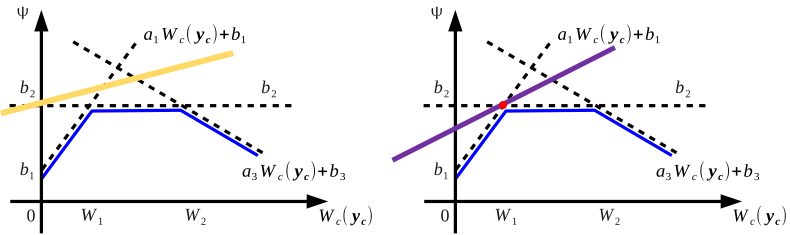
\includegraphics[width=1\columnwidth]{Part2/figures/redundant}
  \caption{\label{fig:redundant} Example lower linear envelope
    with redundant linear functions. On the left figure, the
    solid yellow line is always inactive. On the right figure,
    the solid purple line intersects $line \; 1$ and $line \; 2$
    at the red point. It's only active when $line \; 1$ and $line
    \; 2$ are both active. Both solid lines are redundant linear
    functions hence can be removed without changing their energy
    function.}
\end{figure}
%

To ensure potentials do not contain redundant linear functions
(functions that would never be active), \citename{gouldlearning}
proposed a constraint on parameters of the envelope. The $k$-th
linear function is not redundant if the following condition is
satisfied:
%
\begin{align}
    0
    <
    \frac{b_k - b_{k-1}}{a_{k-1} - a_k}
    <
    \frac{b_{k+1} - b_k}{a_k - a_{k+1}}
    <
    1.
  \label{eq:nonredundant}
\end{align}
%
Another important property of equation~\eqref{eq:min_energy} is
shift invariant (vertically). We write
$\widetilde{\psi}^{H}_c\!(\vy_c)$ by shift
equation~\eqref{eqn:potential2} vertically with an arbitrary
amount $b^{const}\in R$
$$\widetilde{\psi}^{H}_c\!(\vy_c) = \min_{k=1, \ldots, K}
\left\{a_k W_{\!c}(\vy_c) + b_k + b^\textrm{const} \right\}$$
%
Then we have
\begin{align}
  \argmin_{\vy_c} \psi^H_c\!(\vy_c)
  = \argmin_{\vy_c} \widetilde{\psi}^{H}_c\!(\vy_c).
  \label{eq:shift_invariant}
\end{align}
%
Therefore, in the following discussion without loss of generality
we assume $b_1 = 0$ thus $b_k\geq0 \text{\; for \;} k=1,\dots,n$.

\subsection{Exact Inference}
\label{sec:exact_inference}

Exact inference on MRFs has been extensively studied in past
years. Researchers found that, energy functions which can be
transformed into quadratic pseudo-Boolean
functions~\cite{Ishikawa:PAMI03,Ishikawa:CVPR09,Rother:CVPR09}
are able to be minimized exactly using \emph{graph-cuts} like
algorithms~\cite{Freedman:CVPR05,Hammer:1965} when they satisfy
submodularity condition~\cite{Boros:MATH02}.
\citename{Kohli:TR08} and \citename{Gould:ICML2011} adapted those
results to perform exact inference on lower linear envelope
potentials. In this section we mainly focus on describing the
minimum \emph{$st$-$cut$} graph constructed by
Gould~\cite{Gould:ICML2011,gouldlearning} for exact inference of
energy function (equation ~\eqref{eq:min_energy}) containing
lower linear envelope potentials.

Following the approach of \citename{Kohli:CVPR10},
\citename{Gould:ICML2011,gouldlearning} transformed the weighted
lower linear envelope potential in
equation~\eqref{eqn:potential2} into a quadratic pseudo-Boolean
function by introducing $K-1$ auxiliary variables $\vz =
\left(z_1, \ldots, z_{K-1}\right)$ with $z_k\in \{0,1\}$:

\begin{align}
  E^c(\vy_c, \vz) &= a_1 W_{\!c}(\vy_c) + b_1 \notag \\
  &+ \sum_{k = 1}^{K-1} z_k \left( \left(a_{k+1} - a_k\right) W_{\!c}(\vy_c) + b_{k+1} - b_k \right)
  \label{eqn:binary_concave_z}
\end{align}

\noindent for a single clique $c \in \cal C$. Under this
formulation, minimizing the pseudo-Boolean function over $\vz$ is
equivalent to selecting (one of) the active functions(s) from
equation~\eqref{eqn:potential2}. Another important property of
optimized $\vz$ under this formulation is that it automatically
satisfies the constraint
%
$$z_{k+1} \leq z_k$$
%
This property give rise to further development of parameter
vector and feature vector (equation~\eqref{eq:llsvm_param} and
~\eqref{eq:llsvm_feature}) which are used in latent structural
SVM. By introducing latent variables within the energy function,
we can learn richer energy representations than previous
study~\cite{gouldlearning} and solve inference problem exactly
within polynomial number of iterations.

In order to construct the minimum \emph{$st$-$cut$} graph, we
rewrite equation~\eqref{eqn:binary_concave_z} into
\emph{posiform}~\cite{Boros:MATH02}:

\begin{align}
  \label{eqn:posiform}  
  E^c(\vy_c, \vz)
  &= b_1 - (a_1 - a_K) + \sum_{i \in c} a_1 w^c_i y_i \notag\\
  & + \sum_{k = 1}^{K - 1} \left( b_{k+1} - b_k \right) z_k
    + \sum_{k = 1}^{K - 1} \left( a_k - a_{k+1} \right)
    \bar{z}_k\notag\\
  & + \sum_{k = 1}^{K - 1} \sum_{i \in c} \left( a_k - a_{k+1}
    \right) w^c_i \bar{y}_i z_k
\end{align}

\noindent where $\bar{z}_k = 1 - z_k$ and $\bar{y}_i = 1 - y_i$.
$a_1$ is assumed to be greater than $0$ so that all coefficients
are positive (recall we assume $b_1=0$ in section~\ref{sec:llep}
and we have $a_k > a_{k+1}$ and $b_k < b_{k+1}$). Since the energy function~\eqref{eqn:posiform}
is submodular, the \emph{st-min-cut} graph can be constructed 
based on equation~\eqref{eqn:posiform}.


\begin{figure}[t]
  \centering
  \setlength{\tabcolsep}{2pt}
  \begin{tabular}{cc}
    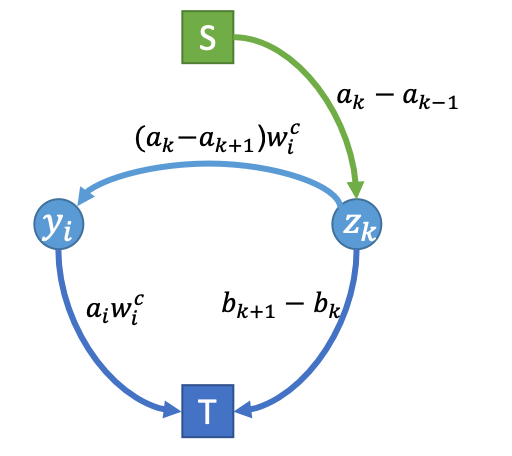
\includegraphics[width=0.47\columnwidth]{Part2/figures/ho.png}&
                                                                         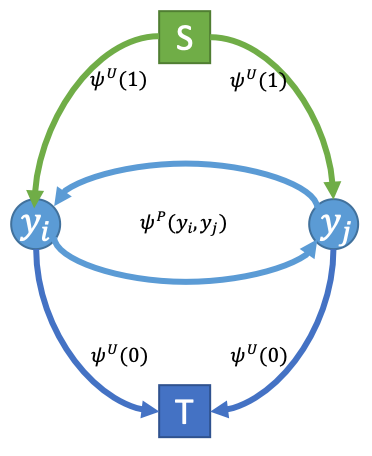
\includegraphics[width=0.37\columnwidth]{Part2/figures/up.png}\\
                                                                         {\small (a)} & {\small (b)} 
  \end{tabular}
  \caption{\label{fig:stmincut} $st$-graph construction for
    equation~\eqref{eqn:posiform}, unary and pairwise terms.
    Every cut corresponds to an assignment to the random
    variables, where variables associated with nodes in the $\gS$
    set take the value one, and those associated with nodes in
    the $\gT$ set take the value zero. With slight abuse of
    notation, we use the variables to denote nodes in our graph.}
\end{figure}


The construction (including unary and pairwise) is explained in
\Figref{fig:stmincut}. Figure (a) denotes construction for
equation~\eqref{eqn:posiform}. For each lower linear envelope
potential edges are added as follows: for each $i \in c$, add an
edge from $y_i$ to $t$ with weight $a_1 w^c_i$; for each $i \in
c$ and $k = 1, \ldots, K-1$, add an edge from $z_k$ to $y_i$ with
weight $(a_{k} - a_{k+1}) w^c_i$; and for $k = 1, \ldots, K-1$,
add an edge from $s$ to $z_k$ with weight $a_k - a_{k+1}$ and
edge from $z_k$ to $t$ with weight $b_{k+1} - b_k$. Figure (b)
denotes construction for unary and pairwise terms (see
\cite{Kolmogorov:PAMI04}). For unary edges (4 edges on both
sides), weights on each edge are corresponding to values in input
unary terms accordingly. For pairwise edges (2 edges in the
middle), both edges share the same weight which equals to the
input pairwise term.

\section[Solving MRFs under LSSVMs]{Solving MRFs under the Latent
  Structrual SVMs (LSSVM) Framework}
\label{sec:opt}

With the inference algorithm in hand, we now can develop the
learning algorithm for weighted lower linear envelope potentials
using the Latent Structural SVMs (LSSVMs) framework. In
\Secref{sec:learning}, we begin by transforming the
equation~\eqref{eqn:binary_concave_z} into a linear combination
of parameter vector and feature vector. A two-step algorithm was
developed to solve the latent structural SVM in
\Secref{sec:mrflssvm_learning_algo}.


\subsection{Transforming Between Representations}
\label{sec:learning}

The latent structural SVM formulation requires that the energy
function be formulated into a linear combination of features and
weights while our higher-order potential is represented as the
minimum over a set of linear functions. However,
in~\ref{sec:exact_inference} we reformulated the piesewise linear
functions into a quadratic pseudo-Boolean function in
equation~\eqref{eqn:binary_concave_z} by introducing auxiliary
variables. Now we show equation~\eqref{eqn:binary_concave_z}
itself is an inner product of parameter vector and feature vector
with latent information. Note that the function can be expanded
as a summation of $2K-1$ terms:

\begin{align}
  \label{eq:originalenergy}
  E^c(y_c,z)
  =&a_1W_c(y_c)+\sum_{k=1}^{K-1}(a_{k+1}-a_k)z_kW_c(y_c) \notag \\
   &+\sum_{k=1}^{K-1}(b_{k+1}-b_k)z_k
\end{align}

Here we use the fact of equation~\eqref{eq:shift_invariant} and
let $b_1=0$. Now we can reparameterize the energy function
as
\begin{align}
  \label{eq:llsvm_innerprod_energy}
  E^c(\vy_c,\vz; \vtheta^H) = \vtheta^{H^T} \! \psi^H(\vy_c,\vz)
\end{align}

\noindent where:

\begin{equation}
\label{eq:llsvm_param}
  \theta_k^H = \left\{
    \begin{aligned}
      & a_1	& \text{for} \ k=1\\
      & a_k-a_{k-1} & \text{for}\ 1< k \leq K\\
      & b_{k+1-K}-b_{k-K} & \text{for} \ K<k\le2K-1\\
    \end{aligned}
  \right.
\end{equation}

\begin{equation}
\label{eq:llsvm_feature}
  \psi_k^H = \left\{
		\begin{aligned}
      & W_c(\vy_c) 	& \text{for} \ k=1\\
      & W_c(\vy_c)\vz_k & \text{for}\ 1<k\le K\\
      & \vz_k & \text{for} \ K<k\le2K-1\\
		\end{aligned}
  \right.
\end{equation}

Under this formulation, similar to \cite{yu2009learning}, the inference problem
can be given by:

\begin{align}
  \label{eq:linenv_full_inf}
  (\mathbf{y}^*_k(\vtheta^H),\mathbf{z}^*_k(\theta^H))=\argmin_{(\mathbf{y}
  \times \mathbf{z}) \in \mathcal{Y} \times \mathcal{Z}}
  \vtheta^{H^T}\cdot\psi^H(\mathbf{y}_k,\mathbf{z}_k)
\end{align}
and
\begin{align}
  \label{eq:linenv_latent_inf}
  \mathbf{z}^*_k(\vtheta) = \argmin_{\mathbf{z} \in \mathcal{Z}}
  \vtheta^{H^T} \cdot \psi^H(\mathbf{y}_k,\mathbf{z}_k)
\end{align}

There are two facts worth to mention. The first fact is that in
our previous construction of minimum $st-cut$ graph the latent
variable $\vz$ is already included. Therefore, we can apply our
inference algorithm directly on our two new formulations. The
second fact is that for equation~\eqref{eq:linenv_latent_inf},
there exists a more efficient algorithm. At training stage, the
ground-truth labels $y_i$ is an input and is completely observed.
Therefore, the term $((a_{k+1}-a_k)W_c(\vy_c)+b_{k+1}-b_k)$ in
equation~\eqref{eq:originalenergy} becomes constant. So we can
infer latent variable $\vz$ explicitly by:
\begin{align}
  \label{eq:linenv_effi_infer_latent}
  z_k^c &=
          \begin{cases}
            0 & \text{if $((a_{k+1}-a_k)W_c(y_c)+b_{k+1}-b_k)\geq0$} \\
            1 & \text{otherwise}.
          \end{cases}
\end{align}

To show the equivalence between
equation~\eqref{eqn:binary_concave_z} and
equation~\eqref{eq:llsvm_innerprod_energy} we consider the
example illustrated in figure~\ref{fig:concave}. Assume the
inferred latent vector $\vz^c=(1,1,0,0)$. Plug it into
equation~\eqref{eq:llsvm_feature} the energy function can be
written as:
\begin{align*}
  E^c(\vy_c,\vz; \vtheta) &=
  \begin{bmatrix}
    a_1\\
    a_2-a_1\\
    a_3-a_2\\
    a_4-a_3\\
    b_2\\
    b_3-b_2\\
    b_4-b_3
  \end{bmatrix}^T
  \begin{bmatrix}
    W_c(\vy_c) \\
    W_c(\vy_c) \\
    0\\
    0\\
    1\\
    0\\
    0
  \end{bmatrix}\\
  &=a_1W_c(\vy_c)+(a_2-a_1)W_c(\vy_c)+b_2\\
  &=a_2W_c(\vy_c)+b_2
\end{align*}

Therefore, assignments inferred by graph-cut algorithm can be
directly encoded into a linear combination by using our latent
structural SVM formulation for learning purpose. The remaining
task is to ensure the concavity of $\vtheta$. We do this by
adding following constraint:

\begin{align}
  \label{eq:concave_constraint}
  A\vtheta\geq\epsilon \text{,\;~~~} A=
                  \begin{bmatrix}
                    1 & \mathbf{0} & \mathbf{0}\\
                    \mathbf{0} & -\mathbf{1} & \mathbf{0}\\
                    \mathbf{0} & \mathbf{0} & \mathbf{P}
                  \end{bmatrix}\in \mathbb{R}^{(2K-1)\times(2K-1)}
\end{align}

\noindent where $-\mathbf{1}$ is a matrix of size $(K-1)\times(K-1)$ and
$\mathbf{P}$ is an identity matrix of size $(K-1)\times(K-1)$.
One subtle problem we found during experiments is that the
algorithm can be stuck with small numerical value. To avoid this
we add small slack variables $\epsilon=\mathbf{1}^{-15}$ on 
those constraints.
\begin{align}
  \label{eq:concave_constraint}
  A\vtheta\geq\epsilon \text{,\;~~~} A=
                  \begin{bmatrix}
                    1 & \mathbf{0} & \mathbf{0}\\
                    \mathbf{0} & -\mathbf{1} & \mathbf{0}\\
                    \mathbf{0} & \mathbf{0} & \mathbf{P}
                  \end{bmatrix}\in \mathbb{R}^{(2K-1)\times(2K-1)}
\end{align}

\subsection{Latent Structural SVM Learning}
\label{sec:mrflssvm_learning_algo}

With the inner product formulation
(equation~\eqref{eq:llsvm_innerprod_energy}) of higher order
energy function, we are able to derive our latent
structural SVM learning algorithm. The energy function (higher
order function together with unary and pairwise functions) can be
written as:
\begin{equation}
  E_{all}(y,z) = \begin{bmatrix}
    \vtheta^H\\
    \theta^{unary}\\
    \theta^{pairwise}
  \end{bmatrix}^T 
  \cdot \begin{bmatrix}
    \psi^H\\
    \psi^{unary}\\
    \psi^{pairwise}
  \end{bmatrix}=\theta_{all}^T\cdot\psi_{all}
\end{equation}
where $\vtheta^H\in \sR^{2K-1}$ is the parameter vector in higher
order equation~\eqref{eq:llsvm_innerprod_energy} of size $2K-1$.
$\theta^{unary}$ and $\theta^{pairwise}$ are both scalars.
$\psi^\textrm{unary} = \sum_i \psi^U_i\!(y_i)$ and
$\psi^\textrm{pairwise} = \sum_{ij} \psi^P_{ij}(y_i, y_j)$.
Therefore, the size of $\theta_{all}$ is $2K+1$.

Plug equation~\eqref{eq:linenv_full_inf} and
equation~\eqref{eq:linenv_latent_inf} into object function in
\cite{yu2009learning}, the latent structural SVM object function
for our problem can be derived as a difference of two convex
functions:

\begin{align}
\label{eq:lssvm_object}
  \min_\theta\bigg(\frac{1}{2}\|\theta\|^2+
  C\sum_{i=1}^{n}\big(\max_{(\mathbf{\hat{y}} \times
  \mathbf{\hat{z}}) \in \mathcal{Y} \times \mathcal{Z}}
  [\theta\cdot\psi(\mathbf{\hat{y}},\mathbf{\hat{z}}) +
  \Delta(\mathbf{y}_i,\mathbf{\hat{y}},\mathbf{\hat{z}})]\big)\bigg)\\
  -C\sum_{i=1}^{n}\big(\max_{\mathbf{z} \in \mathcal{Z}} \theta \cdot
  \psi(\mathbf{y}_i,\mathbf{z})\big)\nonumber
\end{align}

Following \citename{yu2009learning}, we use the two stages
Concave-Convex Procedure (CCCP)~\cite{yuille2002concave} to solve
the optimization problem. We first imputes the latent variables
$\vz$ explicitly by equation~\eqref{eq:linenv_latent_inf}. Namely
solving the ``latent variable completion''
problem~\cite{yu2009learning}:

\begin{align}
  \vz_i^*=\argmax_{\mathbf{z} \in \mathcal{Z}} \theta \cdot
  \psi(\mathbf{y}_i,\mathbf{z})
\end{align}

The inference result $z_i^*$ for $i=1,\dots,n$ is used as
completely observed for later stage. With the latent variable
$z_i^*$ which best explains the ground-truth data $y_i$ in hand,
updating the parameter vector $\vtheta$ reduces to solve the
standard structural SVM problem:

\begin{align}
\label{eq:mrflssvm_object}
  \min_\theta\bigg(\frac{1}{2}\|\theta\|^2+
  C\sum_{i=1}^{n}\big(\max_{(\mathbf{\hat{y}} \times
  \mathbf{\hat{z}}) \in \mathcal{Y} \times \mathcal{Z}}
  [\theta\cdot\psi(\mathbf{\hat{y}},\mathbf{\hat{z}}) +
  \Delta(\mathbf{y}_i,\mathbf{\hat{y}},\mathbf{\hat{z}})]\big)\bigg)\\
  -C\sum_{i=1}^{n}\big(\theta \cdot
  \psi(\mathbf{y}_i,\mathbf{z}_i^*)\big) \nonumber
\end{align}

The last problem remaining is the initialization method. Because
our objective function~\eqref{eq:mrflssvm_object} is not convex
and the CCCP algorithm is only guaranteed to converge to a local
minimum or saddle point\cite{yuille2002concave}, initialization
of $\vtheta$ might affect the performance of our algorithm. Since
there are no theoretical solution for this problem, we propose an
empirical initialization algorithm in \Algref{alg:init_theta}.

\begin{algorithm}[ht]
  \begin{algorithmic}[1]
    \STATE{$gap=\frac{1}{K}$, $a_1=\sU(0,1e6)$, $b_1=0$,
      $sp_1=(0,0)$, $w_0=0$, $counter=2$} \FOR{each
      clique $c\in \gC$} \STATE{Compute weighted clique value
      $w_c=W_c(y_C)$} \IF{$w_c-w_{c-1}>gap$}
    \STATE{$upbound = a_{counter}w_c+b_{counter}$\\
      $sp_{counter}=(w_c,\sU(upbound-0.5,upbound))$\\
      Calculate $a_{counter}$ and $b_{counter}$ using
      $sp_{counter-1}$ and $sp_{counter}$\\
      $counter=counter+1$}
    \ENDIF
    \ENDFOR
    \STATE{If $counter<K$, remaining $a$s and $b$s are all set to
      be $a_{counter}$ and $b_{counter}$} \STATE{Calculate
      $\vtheta$ using $\{a_k,b_k\}_{k=1}^K$}
  \end{algorithmic}
  \caption{\label{alg:init_theta} Empirical initialization
    algorithm for $\vtheta$}
\end{algorithm}

We assume that the more evenly distributed of $W_c(Y_c)$ where
$c\in\gC$ on $x$ axis, the more rich representation (number of
linear functions) the energy function should have. In order to
initialize $\vtheta$, we first determine the x-coordinate of
sampled points $sp$. Then we sample its y-coordinate from a
uniform distribution $\sU(upbound,upbound-0.5)$ to add some
randomness in our initialization as well as maintain concavity.
Linear parameters $a_k$ and $b_k$ are later calculated using
those sampled points $sp_k$ and $sp_{k-1}$. At last we encode
$\{a_k,b_k\}_{k=1}^K$ into $\vtheta$ using
equation~\eqref{eq:llsvm_param}.

Our optimization algorithm is summarized in
\algref{alg:learning}.

\begin{algorithm}[hb]
  \begin{algorithmic}[1]
    \STATE{Set $MaxIter = 100$}
    \STATE{ {\bf input} training set $\{\vy_i\}_{i=1}^{n}$, regularization constant $C > 0$,
      and tolerance $\epsilon \geq 0$}
    \STATE{Initialize $\vtheta$ using \algref{alg:init_theta}}
    \REPEAT
    \STATE{Set $iter = 0$}
    \FOR{each training example, $i = 1, \ldots, n$}
    \STATE{compute $ \vz_i^*=\argmax_{\mathbf{z} \in \mathcal{Z}}
      \theta \cdot \phi(\mathbf{y}_i,\mathbf{z}) $}
    \ENDFOR

    \STATE{ {\bf initialize} active constraints set $\gC_i = \{ \}$ for all $i$}
    \REPEAT

    \STATE{solve the quadratic programming problem in
      equation~\ref{eq:mrflssvm_object} with respect to active
      constraints set $\gC_i$ for all $i$ and concavity constraints
      $A\vtheta\geq \epsilon$ to get
      $\hat{\vtheta}$ and $\hat{\vx_i}$}

    \FOR{each training example, $i = 1, \ldots, n$}
    \STATE{compute $\hat{\vy_i},\hat{\vz_i} = \argmin_{\vy}
      E(\vy,\vz; \hat{\vtheta}) - \Delta(\vy, \vz, \vy_i)$}
    \IF{$\hat{\xi}_i + \epsilon \!<\! \Delta(\hat{\vy_i},
      \hat{\vz_i}, \vy_i) -
      E(\hat{\vy_i},\hat{\vz_i}; \hat{\vtheta}) + E(\vy_i, \vz_i^*; \hat{\vtheta})$}
    \STATE{$\gC_i \leftarrow \gC_i \cup \{\vy_i^\star\}$}
    \ENDIF
    \ENDFOR
    \UNTIL{no more violated constraints}
    \STATE{ {\bf return} parameters $\hat{\vtheta}$}
    \STATE{Set $iter = iter+1$}

    \UNTIL{$iter\geq MaxIter$}
    \STATE{ {\bf return} parameters $\hat{\vtheta}$}
  \end{algorithmic}
  \caption{\label{alg:learning} Learning lower linear envelope
    MRFs with latent variables.}
\end{algorithm}

\section{Experiments}
\label{sec:synth-check}

Since the main contribution of our work is extending our previous
approximate formulation of lower linear envelope potentials to an
exactly formulation, it is necessary to compare the performance
of MRF-LLSVMs to previous work~\cite{gouldlearning}. In this
section, we examine our method's effectiveness by comparing our
results with~\cite{gouldlearning,Gould:ICML2011} on a synthetic
checkerboard. In order to demonstrate that our formulation has
the capability to learn a much richer class of energy function's
representation, we experiment our method on three different
problem instances: checkerboard with squares containing
monotonous color~\ref{sec:monot-color-squar}, checkerboard with
squares containing more pixels of one color over
another~\ref{sec:unbal-color-squar} and checkerboard with
uniformly colored squares containing unbalanced
color~\ref{sec:unif-distr-squar}.

\subsection{Experiment Settings}
\label{sec:experiment-settings}

An image of synthetic checkerboard contains $8 \times 8$ pixel
squares. Each square (clique) contains $16 \times 16$ (256)
pixels. The color of each pixel is either black $0$ or white $1$.
Given a ground-truth checkerboard image
$\vy^*=y^*_1,\dots,y^*_{16384}$, the observed unary terms
$\vy=y_1,\dots,y_{16384}$ are generated as followings. Let
$\eta_0$ and $\eta_1$ be the signal-to-noise ratios for the black
and white squares, the unary terms are generated by destroying
groud-truth label to noisy input
\begin{align}
  \label{eq:noisy_checkerboard}
  y_i = \eta_0 \ind{y^\star_i = 0} - \eta_1 \ind{y^\star_i = 1} + \delta_i
\end{align}
where $\delta_i
\sim \sU(-1, 1)$ is additive i.i.d.\ uniform noise. $\ind{x}$ is
an indicator function which equals $1$ when $x$ is true and $0$
otherwise. The task is to recover the ground-truth checkerboard
from the noisy input.

Our MRF is constructed on this image by associating each node in
the MRF to each pixel in the image. Thus our MRF contains $8
\times 8 \times 256 = 16,384$ variables. The energy function used
in this experiment follows equation~\eqref{eq:energyfunction_UPH}
without pairwise terms.

\begin{align}
  \label{eq:syncheck_energy}
  E(\vy;\vtheta)=\theta^U\sum_{i\in \gN}{\phi^U(\vy_i)}+
  \sum_{\vy_c\in \gC}{\phi^H(\vy_c,\vz_c;\vtheta^H)}
\end{align}
where $\phi^U(\vy_i)=\vy_i$ and $\theta^U$ is a scalar weight for
unary terms. $\phi^H(\vy_c,\vz_c;\vtheta^H)=\vtheta^{H\;T} \!
\phi(\vy_c,\vz_c)$ is equivalent to
equation~\eqref{eq:llsvm_innerprod_energy} and added for each
square (clique $c$) in the checkerboard. The number of linear
equations $K$ in equation~\eqref{eq:llsvm_param} is set to be
$10$. The parameters $\theta^U$ and $\vtheta^H$ are learned using
\algref{alg:learning} with $MaxIter=100$. 

\subsection{Monotonous Colored Squares}
\label{sec:monot-color-squar}

\begin{figure}[hb]
  \centering
  \setlength{\tabcolsep}{2pt}
  \begin{tabular}{cc}
    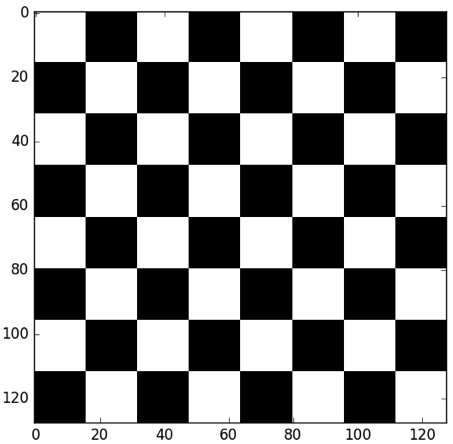
\includegraphics[width=0.5\columnwidth]{Part2/figures/mono_gt.png}&
                                                                            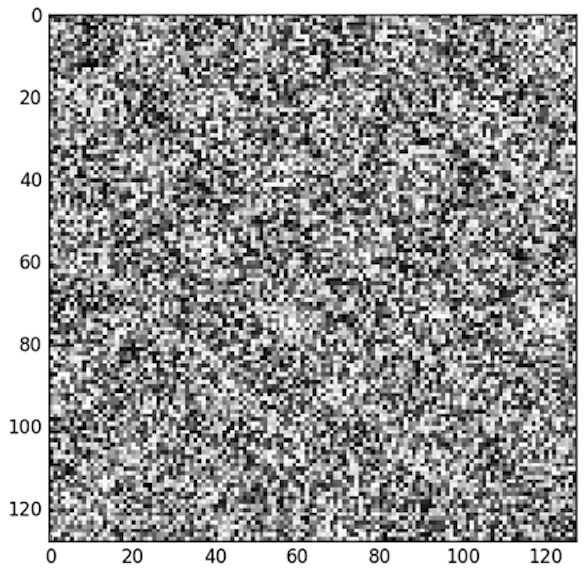
\includegraphics[width=0.5\columnwidth]{Part2/figures/mono_noisy.png}\\
    {\small (a)} & {\small (b)} 
  \end{tabular}
  \caption{\label{fig:mono_checkerboard} Example for monotonous
    colored squares. figure (a) is the ground-truth checkerboard.
    Figure (b) is the noisy input (unary terms) destroyed by
    equation~\eqref{eq:noisy_checkerboard}}
\end{figure}

We first repeat our previous black and white checkerboard
experiment~\cite{Gould:ICML2011,gouldlearning} in order to
examine the correctness of our new formulation. Each clique
(square) $c\in \gC$ in the checkerboard contains either all white
pixels $y_i=1 ,\;\forall i \in c$ or all black pixels $y_i=0
,\;\forall i \in c$. Figure~\ref{fig:mono_checkerboard}
illustrates the ground-truth checkerboard and the noisy input
destroyed by equation~\eqref{eq:noisy_checkerboard} with
$\eta_0=\eta_1=0.1$. Figure~\ref{fig:mono_results} shows the
results of our new method (on the bottom) together with our
previous method~\cite{gouldlearning} (on the top).

\begin{figure}[ht]
  \centering
  \setlength{\tabcolsep}{2pt}
  \begin{tabular}{cc}
    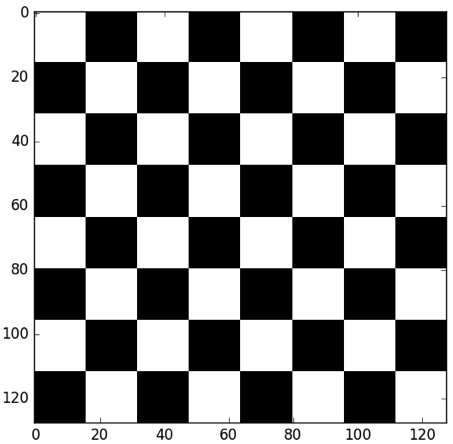
\includegraphics[width=0.3\columnwidth]{Part2/figures/mono_gt.png}&
                                                                              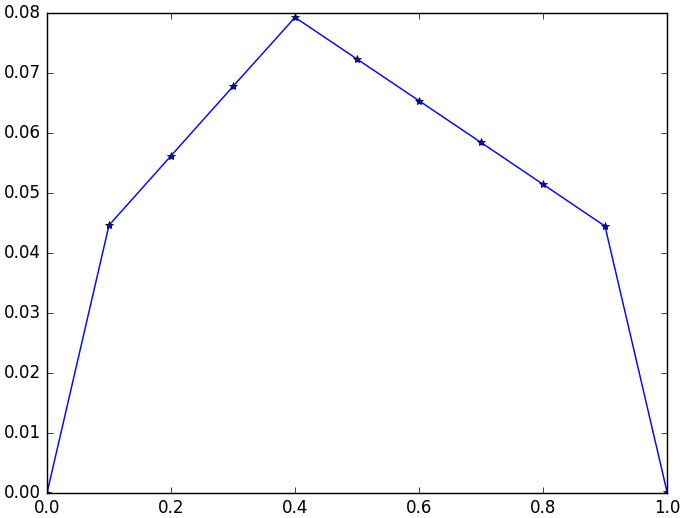
\includegraphics[width=0.4\columnwidth]{Part2/figures/mono_old.png}\\
    {\small (a)} & {\small (b)} \\
    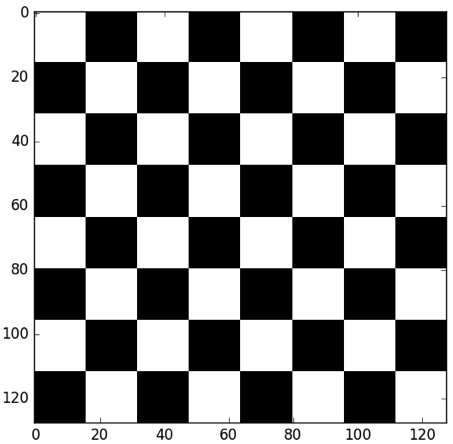
\includegraphics[width=0.3\columnwidth]{Part2/figures/mono_gt.png}&
                                                                              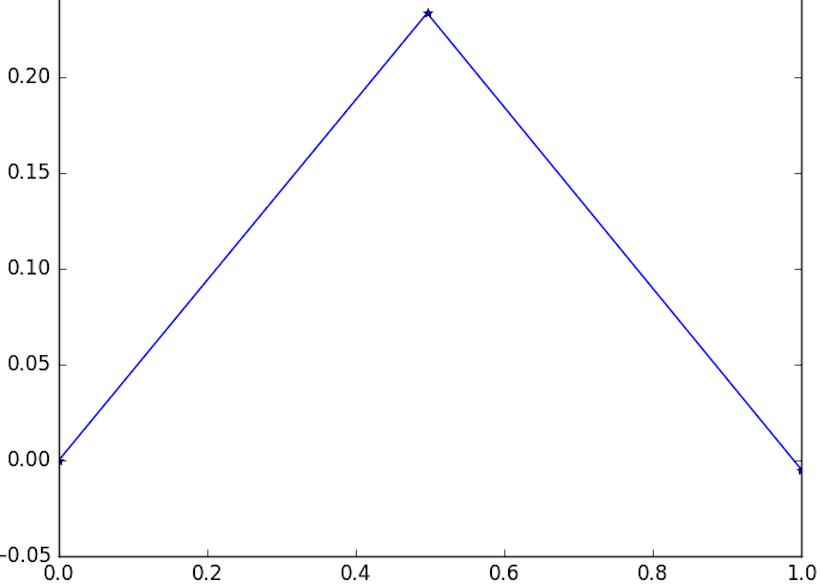
\includegraphics[width=0.4\columnwidth]{Part2/figures/mono_new.png}\\
    {\small (c)} & {\small (d)} 
  \end{tabular}
  \caption{\label{fig:mono_results} Results comparison for
    monotonous colored squares. Figure (a) and Figure (c) are
    inferred checkerboard from our previous and current
    formulation separately. Figure (b) and Figure (d) are lower
    linear envelopes learned by each formulation.}
\end{figure}

From figure~\ref{fig:mono_results} we conclude that both
formulations can recover checkerboard perfectly so our new
formulation's accuracy is as good as previous one. However,
there are significant differences between structural SVM
formulation (previous method) and latent structural SVM
formulation. There are $10$ active linear functions in
figure~\ref{fig:mono_results} (b) while there are only $2$ active
linear functions in figure~\ref{fig:mono_results} (d). Shapes
learned by each formulation are also significantly different.

In general, the second result is more preferable than the first
one. The reason is despite the image contains 64 cliques, there
are only two kinds of squares in the image: completely black and
completely white. Accordingly, our model only see two kinds of
cliques: completely $0$s (black) and completely $1$s (white). In
this case, a lower linear envelope contains two linear functions
is enough for encoding consistency information. This is reflected
in figure~\ref{fig:mono_results} (d) which gives least penalty
(0) when the clique value $W_C(y_c)$ equals either $0$ or $1$. It
gives the highest penalty when $W_C(y_c)$ is in the middle
because our model has least probability seen that in training
data. The results certificates that our latent structural SVM
formulation can learn lower linear envelope exactly. Therefore,
we say that our new method learns more preferable lower linear
envelope.

In terms of computational performance, because our initial point
are generated randomly using \algref{alg:init_theta}, the
performance various between runnings. On average it takes 2
\emph{outer loops} and 47 \emph{inner loops} to converge. Which
means the latent structural SVM formulation spends $3.5$ times
iterations to converge than previous one ($27$ iterations).
Each \emph{inner loop} took under 1s with inference taking about
120ms on a $2.7$GHz dual-core Intel CPU, which is the same as our
previous method.



\subsection{Unbalanced Colored Squares}
\label{sec:unbal-color-squar}

Experiment in section~\ref{sec:monot-color-squar} proves that our
latent structural SVM formulation can learn the lower linear
envelope exactly. In this section we conduct further experiment
to investigate its capability of representing unbalanced input.
The desirable result of this experiment should be the shape of
the lower linear envelope shifting along with the changing of
input data.

We design our checkerboards contain unbalanced colored squares as
shown in figure~\ref{fig:unba_checkerboard}.

\begin{figure}[hb]
  \centering
  \setlength{\tabcolsep}{2pt}
  \begin{tabular}{cc}
    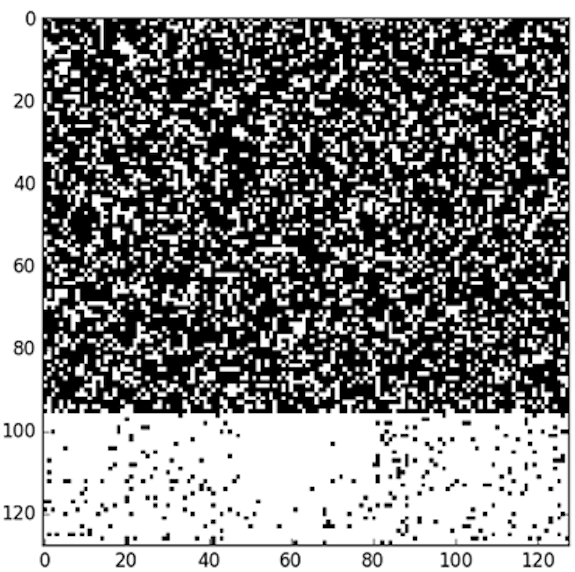
\includegraphics[width=0.5\columnwidth]{Part2/figures/unba_black.png}&
                                                                            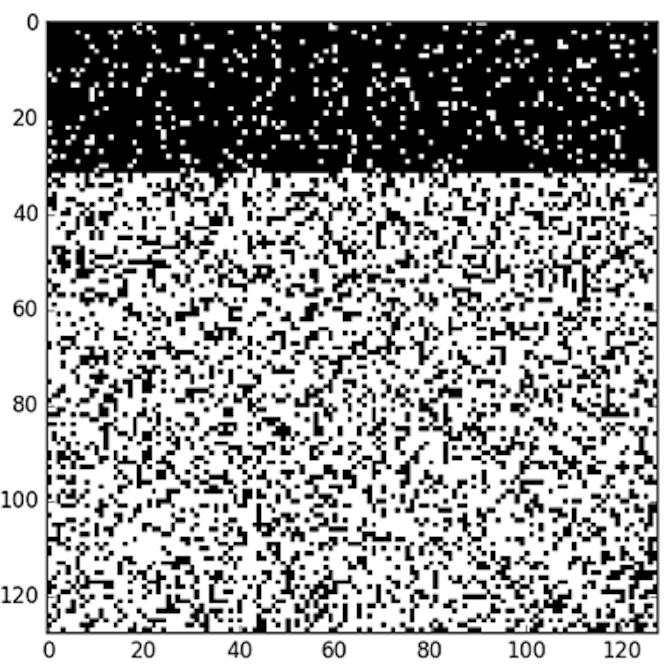
\includegraphics[width=0.5\columnwidth]{Part2/figures/unba_white.png}\\
    {\small (a)} & {\small (b)} 
  \end{tabular}
  \caption{\label{fig:unba_checkerboard} Example for unbalanced
    colored squares. In figure (a) $75\%$ cliques contain more
    than $85\%$ black pixels while $25\%$ cliques contain more
    than $85\%$ white pixels. Figure (b) is the opposite of
    figure (a)}
\end{figure}

As before, figure~\ref{fig:unba_results} shows results learned by
structural SVM (top row) and latent structural SVM (bottom row).
The accuracy performance of both methods are almost the same.
Both methods are able to recover $45\%-50\%$ pixels. The shape of
each formulations' results are both preferable and very similar
when compared to each other. The most significant difference is
the number of linear functions (10 active linear functions v.s.
2). In terms of computational performance, our previous method
only takes $10$ iterations to converge while the latent
structural SVM formulation takes $89$ iterations. Our new method
is much more computational expensive than our previous method.

\begin{figure}[ht]
  \centering
  \setlength{\tabcolsep}{2pt}
  \begin{tabular}{cc}
    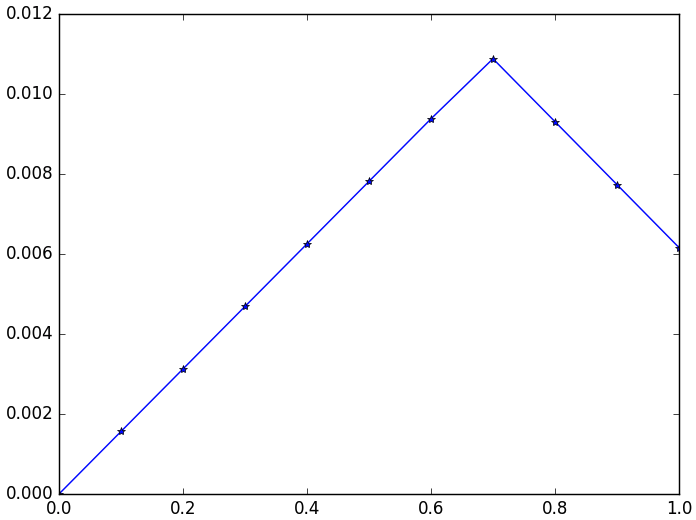
\includegraphics[width=0.5\columnwidth]{Part2/figures/unba_black_res_old.png}&
                                                                              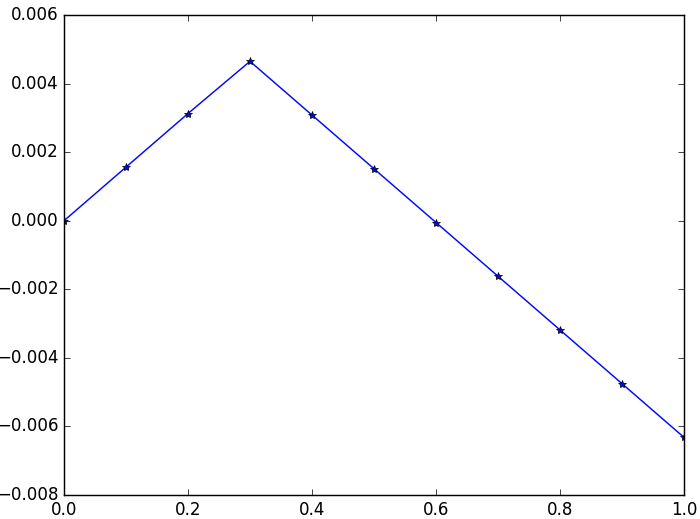
\includegraphics[width=0.5\columnwidth]{Part2/figures/unba_white_res_old.png}\\
    {\small (a)} & {\small (b)} \\
    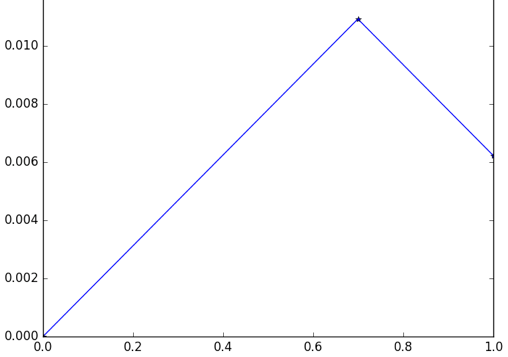
\includegraphics[width=0.5\columnwidth]{Part2/figures/unba_black_res_new.png}&
                                                                              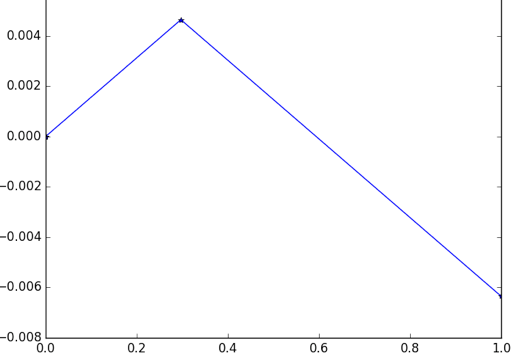
\includegraphics[width=0.5\columnwidth]{Part2/figures/unba_white_res_new.png}\\
    {\small (c)} & {\small (d)} 
  \end{tabular}
  \caption{\label{fig:unba_results} Results comparison for
    unbalanced colored squares. Figure (a) and Figure (b) are
    lower linear (more black and more white) envelopes learned by
    structural SVM. Figure (c) and Figure (d) are learned by
    latent structural SVM.}
\end{figure}

\subsection{Uniformly Colored Squares}
\label{sec:unif-distr-squar}

All of the above experiments show that our new method can
significantly simplify the shape of the lower linear envelope
function while maintaining the inference performance at the same
level. However, one significant cost is the computational
performance. It still remains obscure if there exists any other
advantages. In this section we design a much harder problem.
$W_c(y_c)$ is uniformly distributed from $0$ to $1$.
Figure~\ref{fig:ba_gt} shows the result. The preferable shape of
the lower linear envelope should contain a line which is parallel
to the x-axis.

\begin{figure}[t]
  \centering
  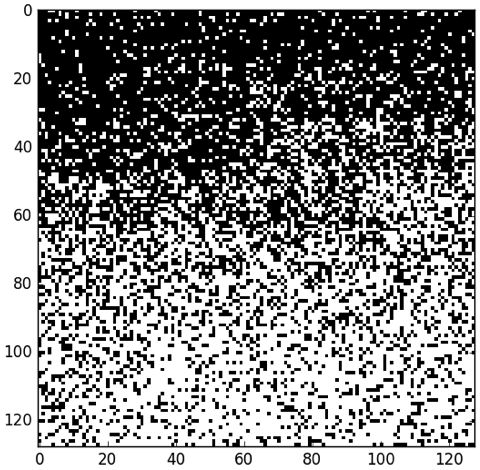
\includegraphics[width=0.5\columnwidth]{Part2/figures/ba_gt.png}
  \caption{\label{fig:ba_gt} Uniformly colored squares example.
    $W_{\!c}(\vy_c) = \sum_{i \in c} w^c_i y_i$ is uniformly
    distributed from $0$ to $1$.}
\end{figure}

Results are shown in figure~\ref{fig:ba_res}. As we can see
that shapes are very different between two formulations. Our
latent structural formulation (figure~\ref{fig:ba_res} (b))
learned a very flat representation of the lower linear envelope
function, which is much preferable, while the structural SVM
formulation preserves much concavity in the shape. This might
because in previous work~\cite{gouldlearning,Gould:ICML2011}
we imposed strict concave constraints on parameter vector
$\vtheta$.

The performance of accuracy also various significantly. Under
this formulation our new method is still able to recover
$45\%-50\%$ pixels while our previous can only recover
$25\%-30\%$ pixels on average. Therefore, our new formulation
finally outperforms previous one. In terms of computational
performance, the new formulation takes $129$ \emph{inner loops}
in total (2 \emph{outer loops}) while our previous formulation
takes $75$ iterations to converge. Although the new formulation
is still more computational expensive than previous one, the gap
decreases significantly.

We consider all of those improvements are due to our new method
is able to learn the lower linear envelope exactly.

One subtle thing is that the linear function on the right side in
figure~\ref{fig:ba_res} (b) decreases sharply which seems
abnormally at first glance. The reason is that we assume $b_1=0$
in section~\ref{sec:llep} which fixes the y-intercept of the
first linear function to be zero. Therefore the last linear
function can be arbitrarily deep while the first linear function
is fixed at the original point.

\begin{figure}[h]
  \centering
  \setlength{\tabcolsep}{2pt}
  \begin{tabular}{cc}
    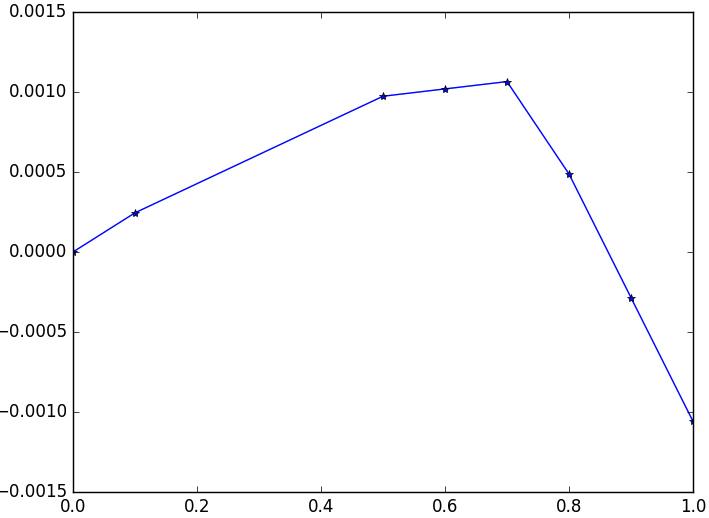
\includegraphics[width=0.5\columnwidth]{Part2/figures/ba_res_old.png}&
                                                                            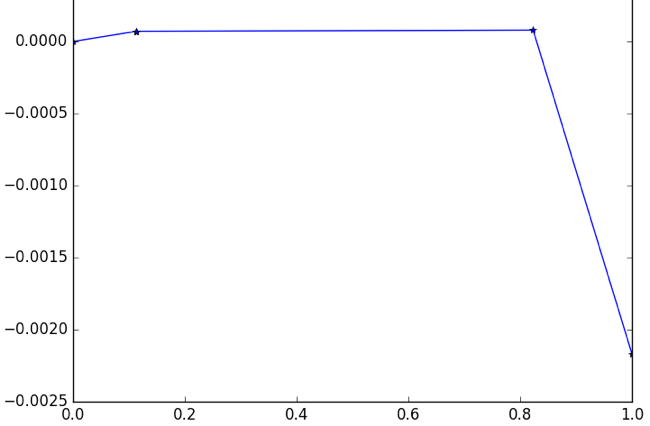
\includegraphics[width=0.55\columnwidth]{Part2/figures/ba_res_new.png}\\
    {\small (a)} & {\small (b)} 
  \end{tabular}
  \caption{\label{fig:ba_res} Results of uniformly colored
    squares experiment. Figure (a) is the result learned by
    structural SVM formulation. Figure (b) is the result learned
    by latent structural SVM formulation.}
\end{figure}

\subsection{Conclusions}
\label{sec:synth-check-conc}

From above experiments we conclude our findings as followings:

\begin{itemize}
\item All of those experiments verified that our latent
  structural formulation is able learn the lower linear envelope
  exactly.
\item In general (see section~\ref{sec:monot-color-squar} and
  section~\ref{sec:unbal-color-squar}), our new method have
  equivalent accuracy performance to our old method (structural
  SVM formulation\cite{Gould:ICML2011,gouldlearning}).
\item In terms of computational performance, the new formulation

  during training. However, it is more efficient during testing
  due to it simplicity for the lower linear envelope potentials.
\item For harder problem (see
  section~\ref{sec:unif-distr-squar}), the new method outperforms
  the previous one significantly. The gap of computational
  performance also decreases a significant amount.
\end{itemize}

%%% Local Variables:
%%% mode: latex
%%% TeX-master: "../thesis"
%%% End:

%% 
%% 
%% 

\chapter{MRF-LSSVM Application: Learning Higher-Order Dynamics on
  China Securities Index (CSI) 300}
\chaptermark{Application: MRF-LSSVM on CSI 300}
\label{cha:mrf_lssvm_app}
It is well known that single the price movement of an individual
stock not only depends on historical records but also highly
correlated to other
stocks~\cite{lo1990contrarian,mech1993portfolio} and may change
in a non-synchronous
manner~\cite{lo1990contrarian,brennan1993investment}. This
correlated yet asynchronous price movement is sometimes referred
to as the lead-lag relationship~\cite{hou2007industry} between a
group of stocks and is thought to arise from the different speed
of information
diffusion\cite{lo1990contrarian,badrinath1995shepherds,mcqueen1996delayed}.
When new information hits the market, some stocks react faster
than others and identification of these leading stocks and their
lead-lag relationships to other lagging stocks provides strong
predictive evidence to the latter\textquotesingle s price
movement.


% Extracting informational price changes from market price data has
% been a long existing challenge in stock trading industry.
% Researchers have developed hundreds of technical
% indicators~\cite{kirkpatrick2010technical} to recognize trend or
% predict volatility in future stock price movement. We are
% inspired by the significant progress in computer vision area
% where researchers developed neural networks which outperform
% hand-crafted features such as SIFT, HOG, and SURF. In this paper
% we try to investigate a multi-task hierarchical RNN neural
% networks in order to replace those hand-crafted technical
% indicators.
However, there are three key challenges in utilizing the lead-lag
relationship: (1) discovering which stock will be affected by
newly arriving information (such as news); (2) identifying the
group ($e.g.$, industry, supply chain, $etc.$) it belongs to along with
the leading and lagging stocks in this group and
modeling their relationships; (3) predicting the price movement of
each stock by jointly considering knowledge in the correlated
group and an individual stock\textquotesingle price movement at
that moment.

The first challenge is extremely difficult, not only because it
requires an expert level of understanding of the finance system and
market dynamics and the stock price, but also
due to a lack of training data. However, according to the
efficient market
hypothesis~\cite{malkiel1970efficient}, stock price reflects all
available market information.
% chli_comment
% Therefore, informative stock price
% changes can be employed as an approximate of market news arrival.
% In this way, the complexity of the first challenge is transformed
% to the detection of informative price changes in individual
% stocks.
%
Economists hitherto to used patterns hidden inside historical
trading prices and volume to predict future price
movements~\cite{fama1966filter,jensen1967random}. As a result,
hundreds of hand-crafted features, known as technical analysis
indicators~\cite{kirkpatrick2010technical}, have been designed.
However, most of these models have stopped generating profitable
signals since the early 1990s~\cite{park2007we}.
% chli_comment Since trading strategies based on technical
% analysis rules are publicly available and easy to replicate,
% informed institutional traders have been motivated to
% manipulate the market price and encourage retail (individual)
% traders to follow their manipulated price to generate excess
% profit~\cite{sun2016decision}.

To overcome these problems and address the first challenge, here
we employ an end-to-end hierarchical
multi-task~\cite{caruana1993multitask} RNN to extract informative
changes from raw market prices without using hand-crafted
features such as technical analysis indicators. Good price
prediction relies on rich representations and a multi-task
framework that can leverage complementary aspects from diverse
tasks~\cite{sogaard2016deep}. Specifically, given raw market
price data, which only contains six features (opening price, low
price, high price, closing price, volume, and amount) at each
time interval, we leverage a hierarchical multi-task network to
first extract features on different tasks and then concatenate
those complementary feature vectors to make the final prediction.

To model lead-lag relationships and address the other two
challenges, we also present a binary Markov Random Fields (MRFs)
with weighted lower linear envelopes as higher order (when the
clique contains more than two nodes) energy
functions~\cite{Kohli:CVPR07,Nowozin:2011,Gould:ICML2011,gouldlearning}.
In our implementation, we treat each stock as a node in MRFs and
each stock\textquotesingle s group with lead-lag relationships as
a maximum clique in MRFs. We use a pre-defined industry
classification list~\cite{ths} as the prior domain knowledge of
each maximum clique for each stock. By using a weighted version
of higher order functions, stocks have higher weights in the
above list can be seen as leading stocks, and vice versa.
Finally, the complexity of modeling dynamics between leading and
lagging stocks becomes encouraging consistency over large cliques
under weighted lower linear envelope potentials. Logits from
hierarchical RNN networks are used as unary features in MRFs. By
minimizing the energy function which contains both unary and
higher order features, we can predict each stock\textquotesingle
s future price movement by jointly considering individual market
price trends together with lead-lag relationships.

% todo: 这样说是否合适
Unlike the first challenge trying to avoid prior knowledge, we
consider being able to embed prior knowledge as an advantage.
Definitions of sectors as well as leading and lagging stocks in
each sector require solid financial industry research.
Statistical evidence learned automatically from market price data
are usually insufficient for determining such relationships.

We demonstrate the effectiveness of the proposed technique using
three popular Chinese stock market indexes, and the proposed
method outperforms baseline approaches. To our best knowledge,
the proposed technique is the first one to investigate
intra-clique relationships with higher-order MRFs on stock price
movement prediction.
  
% todo: 需要4.04分钟引用文献
% We verify our methodology on Chinese stock market because it is
% generally considered less mature than other developed
% countries\textquotesingle thus potentially to be more
% profitable~\cite{bessembinder1995profitability}. Even though
% immature, \citename{fangyan2012} found that the average
% duration of information arrival-conduction-integration-release
% process is $4.04$ minutes. Therefore, a minute-level frequency
% model is mandatory to leverage from lead-lag relationship. To
% our best knowledge, our model is the first one demonstrating
% lead-lag relationship at minute-level frequency on Chinese
% stock market.

To summarize, the main contributions of this paper as follows: 
\begin{itemize}
\item We propose a hierarchical multi-task RNN architecture to
  learn stock price patterns without hand-crafted features. To
  our best knowledge, this is the first work proposing a
  multi-task neural networks for stock price movement prediction.
\item We propose the first model that encode lead-lag
  relationships between stocks using higher-order MRFs.
\item We develop an algorithm to learn the weighted lower linear
  envelope with latent variables as a higher order energy function
  under the latent structural SVM framework. Adding latent variables
  to higher order functions enables our model to learn
  richer representations than previously study~\cite{gouldlearning}.
  Furthermore, our algorithm is not limited to
  stock price movement prediction but can easily be applied
  to other time series tasks and computer vision tasks.
\end{itemize}

In this section, we first introduce 3 stock datasets. Then, we
introduce the parameter settings for our model and training
details. Finally, we select four evaluation metrics and use them
to demonstrate the effectiveness of our proposed model by comparing to
several baseline approaches.

\section{Related Works}
\label{sec:background}

\textbf{Lead-lag relationships:} Lead-lag relationships have long
been recognized in the stock market. They can arise for many
reasons such as information diffusion, sector (industry)
rotation, investment style rotation, event-driven trading, and
asynchronous
trading~\cite{lo1990contrarian,chordia2000trading,conrad1988time,hameed1997time}.
It is generally believed that lead-lag relationships are more
prevalent in firms in the same industry \cite{hou2007industry},
justifying our use of pre-defined industry classification list
\cite{ths} as prior domain knowledge of each
stock\textquotesingle s maximum clique. Several studies
\cite{brennan1993investment,hou2007industry,badrinath1995shepherds,mcqueen1996delayed}
have shown that stocks with larger capital size and higher
liquidity tend to be leading stocks and vice versa. To replicate
potential lead-lag relationships, we assign each stock a
different weight from its corresponding indexes created by the
China Securities Index Company, Ltd. More complicated dynamics
hidden behind a clique of stocks are learned by higher-order
MRFs.

\textbf{Multi-task learning:} \citename{caruana1993multitask}
showed that inductive knowledge learned from multiple tasks can
transfer between tasks and help improving generalization of all
tasks. Many Natural Language Processing (NLP) tasks take
advantage of multi-task frameworks and achieve state-of-the-art
performance while using simple models for each of these tasks
\cite{sogaard2016deep,hashimoto2016joint}. However, as noted
elsewhere \cite{caruana1993multitask,ruder2017overview}, there is
a lack of theory on underpinning a diverse set of tasks and the
hierarchical architecture of the chosen tasks. Recent works
\cite{sogaard2016deep,hashimoto2016joint} apply the principle
that the task complexity should increase according to
hierarchical level, and we do likewise. Because technical
analysis indicators can be categorized into trend, momentum,
volatility and volume~\cite{kirkpatrick2010technical}, and volume
is included in market price data, we propose an architecture that
uses trend and volatility tasks as lower level tasks and price
movement prediction (upward or downward) as a higher level task.
Other task selection and hierarchical designations remain open
for further research.

\section{Methods}
\label{sec:meth}

In this section, we introduce the multi-task RNN-MRFs
architecture which is constructed with two parts. The first part
is a ``Multi-task Market Price Learner", which consists of three
dual stage attention based recurrent neural network
(DARNN)~\cite{qin2017dual} modules. The goal of the first part is
to tackle the first challenge, \ie automatically extracting
informative representations of the raw market price without
considering any hand-crafted feature and technical indicator. The
second part is an ``Intra-clique Predictor'' which is a binary
Markov random fields model with weighted higher order energy
functions. Those higher order functions are applied to sector
lists (used as maximum cliques) defined by financial experts. The
domain knowledge about leading stocks and lagging stocks are
assigned as higher and lower weights in energy function
accordingly. The goal of this part is to tackle the second and
third challenges. Unary features learned by DARNN modules are
jointly employed to maintain higher order consistency among
stocks belonging to the same sector. The detailed architecture is
shown in Figure~\ref{fig:mrfrnn}.

\section{Multi-task Market Price Learner}
\label{sec:mmpl}

Stock price movement can be interpreted from many aspects such as
investors sentiment, temporal patterns and cycles, flow of funds
and market strength, \textit{etc}. Ideal features should
incorporate as many aspects as possible. Multi-task learning
has shown its effectiveness to learn inductive knowledge among
tasks and improve performance as well as generalization
capability~\cite{caruana1993multitask}. Therefore, we propose a
multi-task RNN framework entitled ``Multi-task Market Price
Learner (MMPL)'' to tackle the first challenge: extracting
informational representations from raw market price.

However, as noted elsewhere
\cite{caruana1993multitask,ruder2017overview}, there is a lack of
theory on underpinning a diverse set of tasks and the
hierarchical architecture of the chosen tasks. We follow this
intuition to construct our model. Most technical indicators fall
into four categories: trend, momentum, volatility and
volume~\cite{kirkpatrick2010technical}. Since volume is included
in input for all low-level tasks and we assume that momentum
information can be learned by a high-level task, we propose an
architecture that using trend and volatility tasks as our low-level tasks and price movement prediction (upward or downward) as
the high-level task.

% As an early work under this direction, the main idea is to test
% effectiveness of multi-task framework on stock dataset rather
% than design a dedicated neural network, we directly borrow the
% idea from DARNNs~\cite{qin2017dual} as our basic module because
% of its ability of attending to multiple features. To the best
% of our knowledge, we are the first work proposing a multi-task
% neural network on stock market data.

Multi-task Market Price Learner(MMPL) contains two
levels, three modules of DARNNs. DARNNs~\cite{qin2017dual} are
used as our basic module not only because of its capability of
selecting relevant deriving series as well as temporal features,
but also due to its superior performance for time series
prediction compared to LSTM~\cite{hochreiter1997long} and
attention based LSTM~\cite{attention}. Specifically, the bottom
level contains two separate DARNN modules. They are supervised by
low-level tasks which aim to predict future price as well as
volatility based upon the raw market price data. The key
difference among those modules is the loss function. At the top
level, it is supervised by a high-level task that learns to use
representations extracted by two low-level modules as well as raw
market price data to predict positive / negative price movement
of stocks. Logits of the last layer are passed to Intra-clique
Predictor described in section~\ref{sec:srp} as unary features.

\begin{figure}[t]
  \centering
  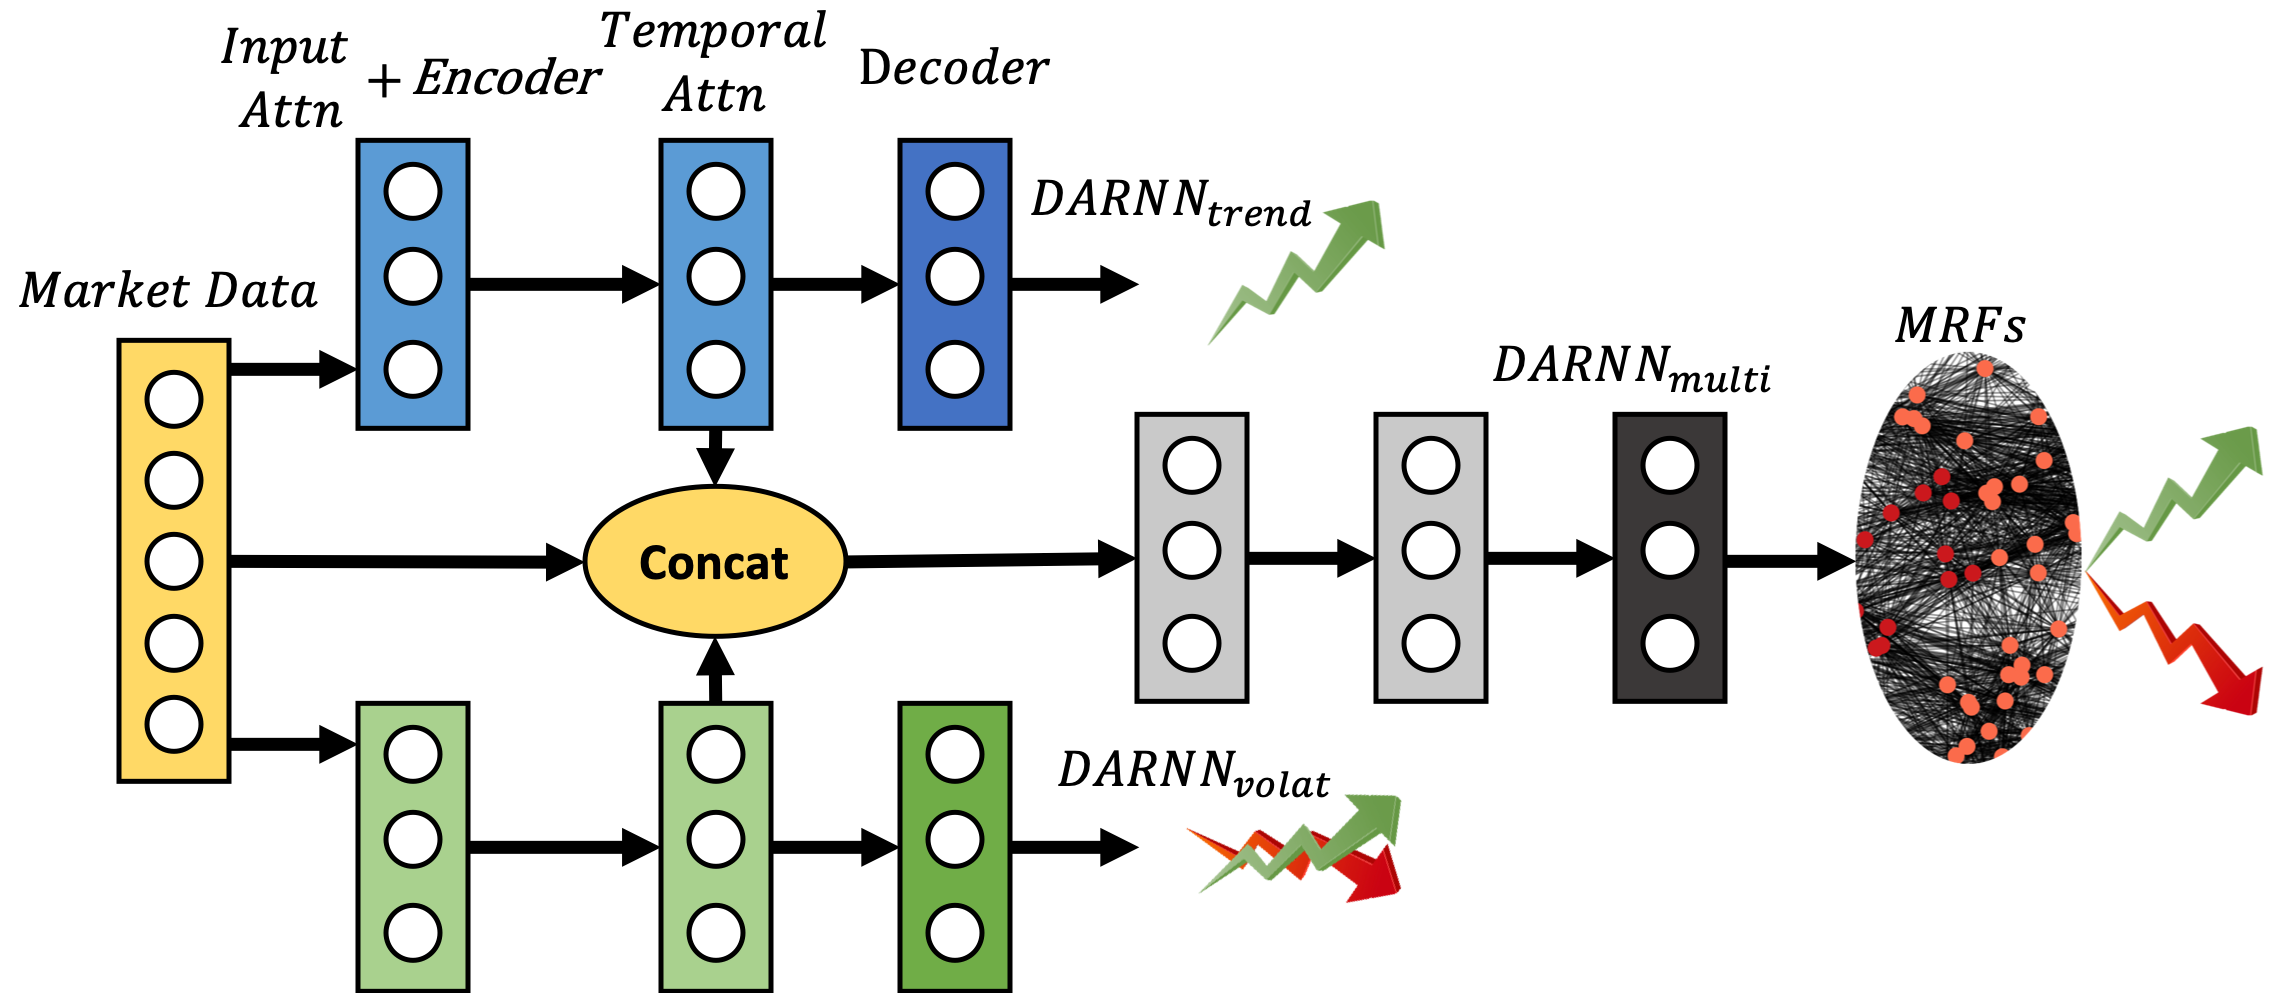
\includegraphics[width=1\columnwidth]{Part2/figures/mmplmrf.png}
  \caption{\label{fig:mrfrnn} Multi-task RNN-MRFs architecture. Note 
  that the output of $\text{DARNN}_{\text{multi}}$ only corresponds to one 
  node's unary feature in MRFs.}
\end{figure}

All three DARNN modules share the same raw market price data.
Here, we denote the time-series dataset as $\mX$ where
$\mX=(\vx_1,\vx_2,\dots,\vx_T)\in \sR^{N\times T}$. We use
$\vx^n=(x_1^n,x_2^n,\dots,x_T^n) \in \sR^T$ to denote a driving
series of $T$ time-steps and $\vx_t=(x_t^1,x_t^2 ,\dots
,x_t^N)\in \sR^N$ to denote a snapshot at time-step $t$ of all
$N$ features.

For both DARNN modules at the low level, the input is $\mX \in \sR^{5\times T}$
which contains $5$ exogenous driving series, \textit{i.e.}, opening price, low
price, high price, volume, amount and $1$ target series $\vy =
(y_1,y_2,\dots,y_T) \in \sR^T$. These two modules
aim to predict target series $y_{t+p}$ in the next $p$ time
steps:

$$\hat{y}_{t+p} = \text{DARNN}(y_1,\dots,y_{t},x_1,\dots,x_t)$$

The target series $\vy_{\text{trend}}$ of
$\text{DARNN}_{\text{trend}}$ is the closing price. The target series
$\vy_{\text{volat}}$ of $\text{DARNN}_{\text{volat}}$ is the
standard deviation of closing price over $M$ constant time-steps.
In our implementation we set $M=10$. We use Mean Squared Error
(MSE) as the loss function to train those two modules separately.

To construct the high level DARNN module, which aims to predict
the price movement, we concatenate context vectors $\vc_T$ from
each of low level DARNN module's encoder and raw market price
matrix as the input. The target series $\vy^{\text{binary}}$ is
constructed by the sign function $y_t^{\text{binary}} =
sign(y_{t+p}-y_t)$ where $y_t$ denotes closing price at time-step
$t$. We use cross-entropy as loss function to train the final
$\text{DARNN}_{\text{multi}}$. Logits (outputs before going
through \emph{softmax}) of $\text{DARNN}_{\text{multi}}$ are then
passed to Intra-clique Predictor as unary features.

In order to train MMPL together with MRFs in an end-to-end
manner, we follow the subgradient method proposed by
\citename{witoonchart2017application}. Since our inner loop
proposed in section~\ref{sec:mrflssvm_learning_algo} is actually
a latent structural SVM. Only gradients of parameters and feature
functions need to be updated. In our framework, outputs of
MMPL (Logits of $\text{DARNN}_{\text{multi}}$) are only used as unary features in MRFs' energy functions,
our back-propagation rules can be defined by taking derivative of the objective function \textit{w.r.t} $\vw^U$  defined in
~\eqref{eq:mrflssvm_object}:

\begin{align}
  \label{eq:der_w}
  \frac{\partial L}{\partial \vw^U} = \psi^U(y)-\psi^U(y^*)
\end{align}

\noindent where $y$ is the ground-truth label and $y^*$ is
inferenced label. $\psi^U$ is unary feature
function described in section~\ref{sec:llep}, here it denotes
logits calculated from $\text{DARNN}_{\text{multi}}$. $\vw^U$ is
unary parameter defined in energy function~\eqref{eq:energyfunction_UPH}.
Equations \eqref{eq:der_w} can be directly plugged
into sub-gradient algorithm proposed in \cite{witoonchart2017application}.
Other configurations stay the same with their algorithm.

\subsection{Intra-clique Predictor}
\label{sec:srp}

In this section, we show how to construct an ``Intra-clique
Predictor" to model lead-lag relationships and address the other
two challenges as mentioned in the introduction. Specifically, we
present a binary Markov Random Fields (MRFs) with weighted lower
linear envelopes as higher order (when the clique contains more
than two nodes) energy functions. Note that the algorithm
proposed here is a general framework for classification tasks.
Besides time series classification, it can also be applied to other tasks such as computer vision.

Pairwise energy function is included only to show our framework
applies to general cases. To our best knowledge, there is no
public available definition of pairwise relationship between
stocks. In our implementation, we use logits from MMPL as unary
function and weighted lower linear envelopes as higher order
function to encode lead-lag relationships. Pairwise features are
excluded.

The detail of the optimization algorithm is summarized in
\algref{alg:learning_app}. As we mentioned in
\appref{sec:train_detail}, although we proposed an end-to-end
subgradient algorithm is section \ref{sec:mmpl}, MRFs updated by
such algorithm take too many iterations to converge. Therefore,
we propose a two-stage training procedure. At first stage, MMPL
and MRFs are trained separately. Therefore, MRFs can take
advantage of the efficient latent structural SVM and converge in
a polynomial number of iterations. After all those models are
converged, we then combine them together to conduct end-to-end
training. Note that the CCCP Inner Loop in
\algref{alg:learning_app} is actually solving standard structural
SVM problem. Therefore, at the second stage, we use subgradient
algorithm proposed in section~\ref{sec:mmpl} to replace the CCCP
Inner Loop. Other settings remain the same.

\section{Dataset and Model Settings}
\label{sec:dataset}

To demonstrate the effectiveness of higher order consistency, we
choose three exclusive and the most famous stock indexes on Chinese
stock market to build our input datasets. Their index codes are:
CSI (China Securities Index) 200, CSI 300 and CSI 500 which
contain 200, 500 and 300 constituent stocks respectively. The CSI
300 index selects most liquid A-share stocks. It aims to reflect
the overall performance of China A-share market. The CSI 200 and
500 indexes aim to reflect the overall performance of mid-to-large
and small-to-mid capital A-shares respectively.

All these indexes are exclusive and are refined on a yearly
basis. In this paper, we use fixed versions on 30-JAN-2015. We
then collect their constituent stocks' minute-level data from
05-JAN-2015 to 29-DEC-2017. On Chinese stock market each trading
day has 4 trading hours. So there are 240 samples (minutes) for
each normally traded stock on each day. Each sample contains 6
features: opening price, high price, low price, closing price,
volume, and amount. \footnote{During this period, there are some
  stocks de-listed (SZ000024, SH600485, SH600832 in CSI 200;
  SZ000693, SZ000748, SZ000982 in CSI 500; SH600485, SH600832,
  SZ000024, SH601299 in CSI 300). Therefore, in total we collect
  197, 497 and 296 stocks during this period respectively.} For
each stock, the first $80\%$ days are used to construct the
training set and the last $20\%$ days are used as test set.
Approximately training set and test set contain $33.6$ million
and $4.2$ million samples, respectively. $49.5\%$ of them are
positive movements, $0.3\%$ of them stay unchanged and $50.2\%$
of them are negative movements. For binary classification task,
we follow \citename{mitchell2001characteristics}'s approach and
label all positive movement samples $1$ and $0$ for the other
samples. More labeling details are described in appendix
\ref{sec:train_detail}.

\begin{table}[H]
\centering
\small
\caption{Technical Indicators Selection}
\begin{tabular}{|c|c|} \hline
  Category&Indicator Name\\ \hline
  Momentum& Awesome Oscillator, Money Flow Index\\ \hline
  Volume& \makecell{Chaikin Money Flow\\ On-balance volume mean}\\ \hline
  Volatility& Bollinger Bands (Upper and Lower Bands)\\ \hline
  Trend& \makecell{Average Directional Movement Index\\Moving Average Convergence Divergence}\\ \hline
\end{tabular}
  \label{tab:ta}
\end{table}
To demonstrate the benefits of multi-task RNN over manually designed
technical indicators, we construct technical
indicators datasets. We select 8 most popular indicators, 2 from each
category~\cite{kirkpatrick2010technical} shown in Table
\ref{tab:ta}. In implementation, we use open source package
\emph{Technical Analysis Library in
  Python\footnote{https://github.com/bukosabino/ta}} to calculate
those indicators and all hyperparameters are using package's
default settings without any prior expert knowledge involved
with. After technical indicators calculation, these 8 new
features are concatenated to above market price dataset (5
features at each minute). So the final input dataset for each
single task model contains 13 features in total. Before feeding
into models, we normalize each stock with \emph{z-score} function
using standard deviation and mean calculated in the training set.

For brevity, we denote market price dataset which only contains
$5$ features as \textbf{Market} and the concatenated $13$
features dataset as \textbf{Indicator}. As discussed in
section~\ref{sec:mmpl}, closing price at time $t$ can be directly
used as regression target for $\text{DARNN}_{\text{trend}}$.
Standard deviation of closing price with a window size of $10$ is
used as regression target for $\text{DARNN}_{\text{volat}}$. The
dimensions of hidden state and cell state are fixed as 32 for
$\text{DARNN}_{\text{trend}}$ as well as
$\text{DARNN}_{\text{volat}}$, and 128 for
$\text{DARNN}_{\text{multi}}$. More training details are
described in appendix \ref{sec:train_detail}.

\section{Results}
\label{sec:res}

In order to demonstrate the effectiveness of our framework, we
compare 3 baseline methods, \textit{i.e.},
LSTM~\cite{hochreiter1997long}, attention based LSTM
Encoder\_Decoder~\cite{attention}, and DARNN~\cite{qin2017dual}
on 3 different Chinese Securities Indexes with and without
technical analysis indicators as inputs. Results are summarized
in Table~\ref{tab:result}. All results are reported over the test
sets. We select four metrics (Accuracy, Precision, Recall and F1
Score) as evaluation metrics to justify the effectiveness of the
proposed approach. They are calculated by collecting all
predicted labels of constituent stocks in each CSI index.

\begin{figure}[t]
  \centering
  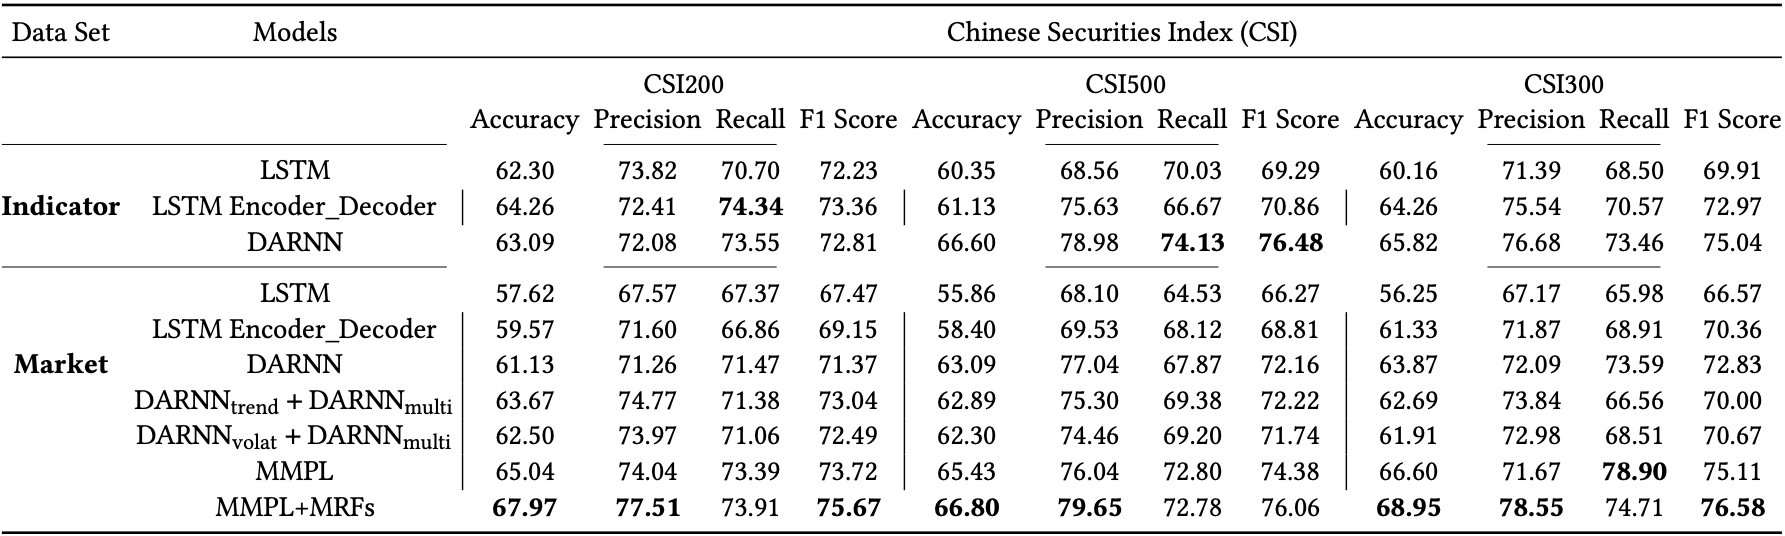
\includegraphics[width=1\columnwidth]{Part2/figures/table_results.png}
  \caption{\label{tab:result} Results: baselines and ablation
    studies. All models have a window size (lag steps) of 20 and
    predict price movement label at the next time step.}
\end{figure}


\subsection{Effectiveness of multi-task framework}

As mentioned earlier, to demonstrate effectiveness of multi-task
framework, we use \textbf{Indicator} dataset, which contains both
market price data and technical analysis indicators as inputs for
baseline approaches and \textbf{Market} dataset which only
contains market price data as inputs for MMPL (multi-task RNN) as
well as baseline methods. For DARNN, we use a hidden size of
$128$. MMPL's configuration is described in
section~\ref{sec:multi_train}. As we can see in
Table~\ref{tab:result}, single task models (LSTM, LSTM
Encoder\_Decoder, DARNN) tested on \textbf{Market} dataset
(without technical analysis indicators as inputs) generally have
worse performance with all 4 metrics. In particular, performance of
DARNN models tested on \textbf{Indicator} dataset is consistently
better than the ones on \textbf{Market} dataset. This proves that
even with hand-crafted features, deep learning models can still
benefit from diversified and complementary features.

To test the effectiveness of multi-task framework, we conduct
ablation study with only one low-level task (\quad
$\text{DARNN}_\text{trend}$ \quad or \\
$\text{DARNN}_\text{volat}$) together with the high-level task
module $\text{DARNN}_\text{multi}$. Results indicate that these
two variants have comparable or slightly worse result than DARNN
on \textbf{Market}. This may because single task model does not
provide diversified features while have more parameters than
DARNN. Finally, MMPL outperforms all single task models and
baseline methods on \textbf{Market}. This suggests that
diversified and complementary tasks can help MMPL extract
effective features. Specifically, by comparing MMPL and DARNN on
\textbf{Market} as well as \textbf{Indicator}, we can see that
MMPL generally outperforms DARNN on CSI200 and CSI300 indexes and
is slightly worse than DARNN on \textbf{Indicator} of CSI500
index. We can conclude that by using multi-task RNNs, we can
extract better or at least comparable features compared with
hand-crafted features.

\subsection{Effectiveness of higher-order MRFs}
In Table~\ref{tab:result}, we can observe that MMPL-MRFs
framework consistently outperforms other baselines on all 3 CSI
index constituent stocks. It shows evidence that higher-order
energy function can help with encoding clique level consistency
thus improving overall prediction performance. One interesting
point to note is that the recall rate of MMPL-MRFs is constantly
lower than other baselines. This can be seen as a trade off
between accuracy and recall rate. However, it is worth to mention
that for stock price movement prediction, high accuracy and
precision are much preferred than recall rate. Another
interesting phenomenon is that MMPL-MRFs gives more improvement
on CSI200 and CSI300 while less improvement over DARNN trained
with technical analysis indicators on CSI500. One possible reason
is that CSI200 and CSI300 select most liquid and representative
stocks in Chinese stock market. Those stocks exhibit much
stronger and higher order consistency than illiquid stocks.
CSI500 selects small-mid capital stocks which are less liquid and
contains much more noisy movements.

In the training stage, our algorithm converges in 4 to 19
CCCP outer loops. The average inference time of graph-cut
algorithm is 34 seconds.

\subsection{Visualization of higher-order consistency}

In order to further investigate higher-order MRFs' effectiveness,
we design a heat-map to visualize CSI300 index intra-clique
higher-order relationship in figure~\ref{fig:consistency}.

\begin{figure*}[t]
  \centering
  \setlength{\tabcolsep}{20pt}
  \begin{tabular}{cc}
  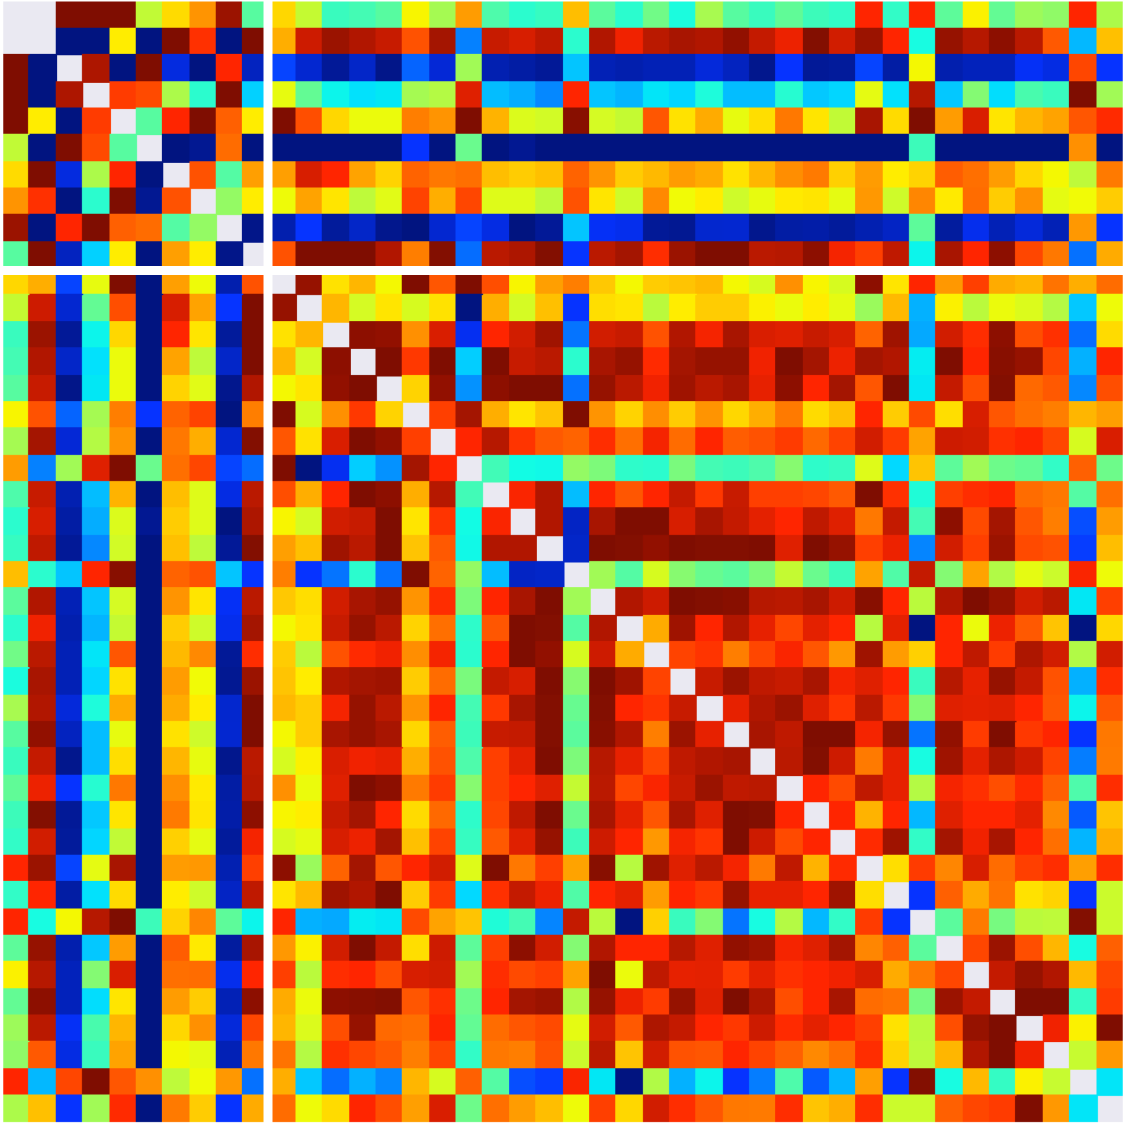
\includegraphics[width=0.4\columnwidth]{Part2/figures/gt.png}&
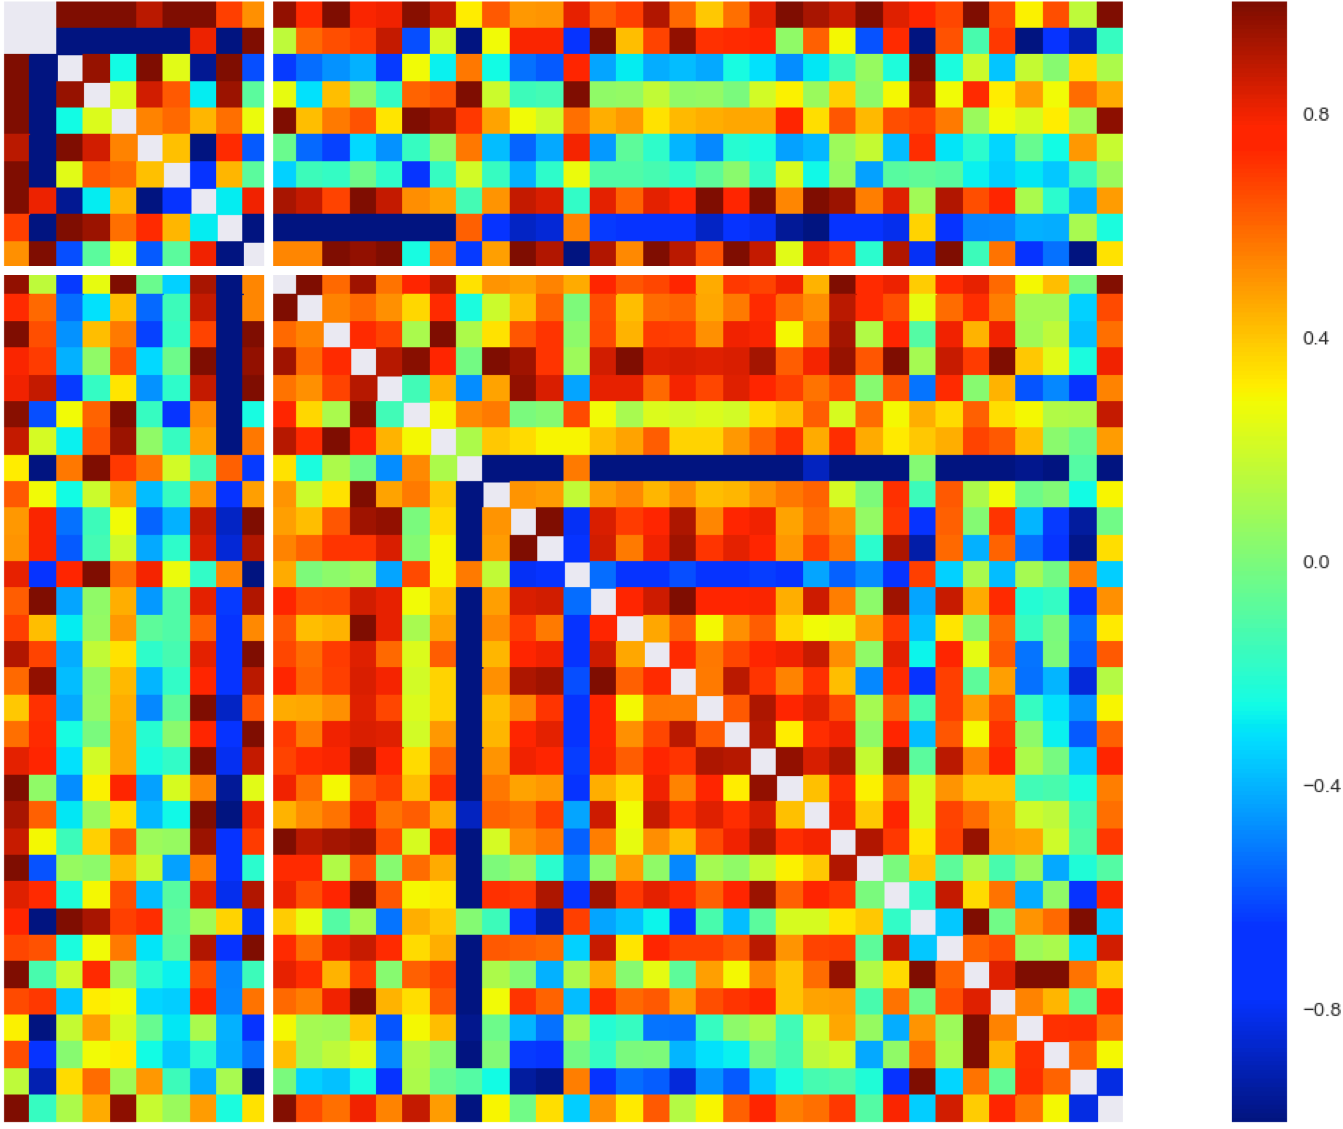
\includegraphics[width=0.48\columnwidth]{Part2/figures/mmpl.png}\\
{\small (a) Ground-truth} & {\small (b) MMPL }\\
    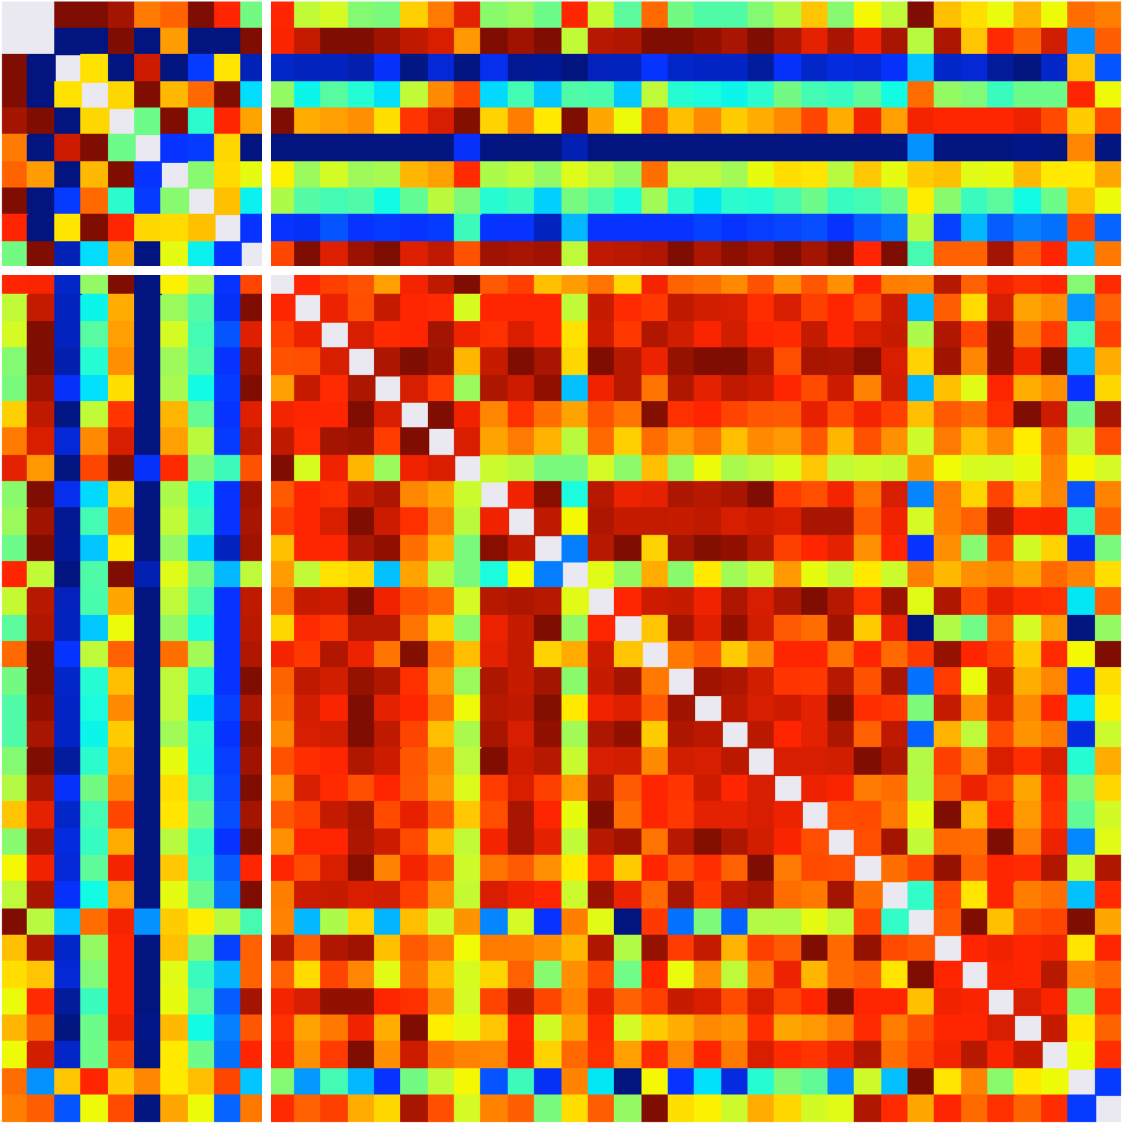
\includegraphics[width=0.4\columnwidth]{Part2/figures/mrf.png}\\
{\small (c) MMPL-MRFs}\\
  \end{tabular}
  \caption{\label{fig:consistency} Higher order consistency
    visualization. (a) is calculated
    directly from ground truth labels on test set.
    (b)
    is calculated using predicted labels of MMPL without MRFs on the
    test set.
    (c), we use predicted labels of
    MMPL-MRFs on test set as inputs.}
\end{figure*}

We first select two sectors: nonferrous metal sector, which
contains 10 constituent stocks, and infrastructure sector, which
contains 35 constituent stocks from CSI300 index \footnote{These
  two sectors are selected only because painting many sectors in
  one figure would be too messy to interpret and those two
  sectors have appropriate clique size (number of stocks) for
  visualization. Conclusions from these two sectors also apply to
  other sectors}. We then measure consistency level between each
two of these constituent stocks. In order to capture their
temporal relationship, we propose a novel consistency measure
which is calculated on temporal intervals.
% Let $\C\in\{\text{Nonferrous Metal},\text{Infrastructure}\}$
% denotes one clique. $\by_c=\{\by_i \in \C\}$ denotes a set of
% time-series $\by_i^T=\{y_i^1,y_i^2,...,y_i^T\}$ for all stocks

Let $\vy_i^T=\{y_i^1,y_i^2,...,y_i^T\}$ denotes time-series for
stock $i$. $y_i^t\in \{0,1\}$ is the binary price movement label
at time $t$. We segment time-series $\vy_i^T$ into
$N=\lceil\frac{T}{P}\rceil$ non-overlapping intervals
$\{y_i^n,y_i^{n+1},...,y_i^{n+P}\}$ with fixed length $P$. For
any two stocks $i$ and $j$, we calculate the difference
$d_{ij}^n=\sum_n^{n+P}{y_i^n}-\sum_n^{n+P}{y_j^n}$ of how many
times positive price movement happen in the $n$-th time interval
in each stock. Then the consistency level $c_{ij}$ between stocks
$i$ and $j$ can be calculated via a $\ell_1\text{norm}$:
$$c_{ij}=-\|\mathbf{d}_{ij}\|_1$$
\noindent where
$\mathbf{d}_{ij}=\{d_{ij}^1,d_{ij}^2,...,d_{ij}^N\}$. We
normalize $c_{ij}$ into interval $[-1,1]$. Each entry in
figure~\ref{fig:consistency} denotes a consistency level measure
$c_{ij}$. The larger the $c_{ij}$ is, the higher of consistency
level between stock $i$ and stock $j$, the color of corresponding
entry is closer to red, and vice versa. As we mentioned, the average duration of information
arrival-conduction-integration-release process is 4.04 minutes~\cite{fangyan2012}.
Since which stock is leading at each time interval is elusive, we
set $P=9$ when calculating consistency measures.

As we can see in Figure 4(a), there is a significant red square
area, which means ground-truth heat-map shows strong intra-clique
consistency. This is an evidence that higher-order relationships
do exist within clique of stocks. However, in Figure 4(b), the red
square area is fragmented into many little pieces. The whole
area's color is closer to blue when compared to ground-truth
heat-map, which means that MMPL captures little higher-order consistency.
The reason we still can observe a shape of red square
is that the accuracy of MMPL model on CSI300 is $66.6\%$.
However, we can still conclude that the accuracy of single MMPL
model mainly comes from unary features and it fails to capture
higher order consistency of different stocks belonging to the same clique.
On the contrary, even though MMPL-MRFs model's accuracy on CSI300
index is only $2.35\%$ better than MMPL model, we can observe
that heat-map Figure 4(c) is more close to ground-truth heat-map than
heat-map Figure 4(b). There is a much clear red square and the number of
small fragments in red area is also less than Figure 4(b). We can
conclude that MMPL-MRFs models learn to utilize both unary
features from MMPL as well as higher-order relationships encoded
in MRFs.

\section{Conclusions}
\label{sec:conc}

Here we show how to model individual stock price predictions
without hand-crafted features and encode lead-lag relationships
between stocks using weighted higher-order MRFs. A multi-task
neural network framework - Multi-task Market Price Learner (MMPL)
- is proposed to automatically extract diversified and
complementary features from individual stock price sequences.
Features learned by MMPL are passed to a binary MRF with a
weighted lower linear envelope energy function to utilize
intra-clique higher-order consistency between stocks. An
efficient latent structural SVM algorithm is designed to learn
MRFs in polynomial time. Finally, the MRFs and MMPL are trained
end-to-end using the sub-gradient algorithm. Extensive
experiments are conducted on three major Chinese stock market
indexes, and the proposed MMPL-MRFs achieve the best accuracy on
all three indexes.

Our work provides a number of directions for future research. In
this work we proposed a multi-task recurrent neural network for
stock price prediction. While we directly use DARNN as a proof of
concept, other, more dedicated architectures are worthy of
exploration. As well as time series tasks, we can also
investigate how the latent SSVM framework performs on computer
vision tasks. Another interesting direction is to investigate the
implicit relationship between the expert-defined index list and
graph RNN~\cite{you2018graphrnn}, which could further help to
reduce the domain knowledge required by our framework.

%%
%% The acknowledgments section is defined using the "acks" environment
%% (and NOT an unnumbered section). This ensures the proper
%% identification of the section in the article metadata, and the
%% consistent spelling of the heading.

\section{Training Details}
\label{sec:train_detail}

\subsection{Initialization of lower linear envelope}
\label{sec:sup_init}

We assume that the more evenly distributed of $W_c(Y_c)$ where
$c\in\cal C$ on $x$ axis, the more rich representation (number of
linear functions) the energy function should have. In order to
initialize $\vtheta$, we first determine the x-coordinate of
sampled points $sp$. Then we sample its y-coordinate from a
uniform distribution ${\cal U}(\text{upbound},\text{upbound}-0.5)$ to add some
randomness in our initialization as well as maintain concavity.
Linear parameters $a_k$ and $b_k$ are later calculated using
those sampled points $sp_k$ and $sp_{k-1}$. At last we encode
$\{a_k,b_k\}_{k=1}^K$ into $\vtheta$ using
equation~\eqref{eq:llsvm_param}. This algorithm is summarized in
\algref{alg:init_theta}.

\begin{algorithm}[h]
  \begin{algorithmic}[1]
    \STATE{$gap=\frac{1}{K}$, $a_1={\cal U}(0,1e6)$, $b_1=0$,
      $sp_1=(0,0)$, $w_0=0$, $counter=2$} \FOR{each
      clique $c\in \cal C$} \STATE{Compute weighted clique value
      $w_c=W_c(y_C)$} \IF{$w_c-w_{c-1}>gap$}
    \STATE{$upbound = a_{counter}w_c+b_{counter}$\\
      $sp_{counter}=(w_c,{\cal U}(upbound-0.5,upbound))$\\
      Calculate $a_{counter}$ and $b_{counter}$ using
      $sp_{counter-1}$ and $sp_{counter}$\\
      $counter=counter+1$}
    \ENDIF
    \ENDFOR
    \STATE{If $counter<K$, remaining $a$s and $b$s are all set to
      be $a_{counter}$ and $b_{counter}$} \STATE{Calculate
      $\vtheta$ using $\{a_k,b_k\}_{k=1}^K$}
  \end{algorithmic}
  \caption{\label{alg:init_theta} Empirical initialization
    algorithm for $\vtheta$}
\end{algorithm}

\subsection{Multi-task training}
\label{sec:multi_train}

To improve accuracy and reduce over-fitting, we add a drop out
layer between input layer and LSTM layer with a ratio of $0.2$.
We also clip and normalize gradients during back-propagation
stage with a maximum norm of $5.0$ to prevent gradient exploding
issue. As pointed out by \citename{lample2016neural}, the
question of ``when should the training schedule switch from one
task to another task?'' or ``should each task be weighted
equally?'' remains open. In our implementation, we follow the
proportional sampling approach described by
\citename{sogaard2016deep}. After a backward pass completed, we
randomly sample a new task as well as its batch data as the next
task to be trained. In practice, we use a proportion of
$[0.25,0.25,0.5]$ for three tasks respectively. This mechanism
helps multi-task model to avoid \emph{Catastrophic Forgetting}
phenomenon which means lower level model forgets learned
knowledge during higher level model back-propagation pass.

Even though we propose an end-to-end training algorithm for MMPL
and MRFs in section~\ref{sec:mmpl}, MRFs inference stage is still
too slow to be trained jointly with MMPL. To overcome this
difficulty, we implement a two stages training procedure. We
first add a \emph{softmax} layer on top of
$\text{DARNN}_{\text{class}}$ and train MMPL separately from
MRFs. We use \emph{Negative Log-likelihood} as the loss function.
At the second stage, after MMPL converge, we remove the
\emph{softmax} layer and re-train it together with MRFs. One
issue we must mention is that, even though we use binary MRFs
which can only predict positive / negative price movement, we
find there is a significant amount of time when stock price
remains no change. We find it benefits the performance a lot if
we treat the classification as a three classes problem rather
than a binary classification problem during the first stage.
Therefore, at the first stage, the \emph{softmax} layer will
output probability for three labels: \emph{negative movement},
\emph{no changes} and \emph{positive movement}. Since binary MRFs
still needs a two dimension input as part of unary energy
function, after the \emph{softmax} layer is removed, we add an
additional linear mapping layer between logits of MMPL and MRFs
at the second stage.

\subsection{End-to-end multi-task RNN-MRFs training}
\label{sec:mrf_train}

\begin{algorithm}[h]
  \begin{algorithmic}[1]
    \STATE{Set $MaxIter = 100$}
    \STATE{ {\bf input} training set $\{\vy_i\}_{i=1}^{n}$, regularization constant $C > 0$,
      and tolerance $\epsilon \geq 0$}
    \STATE{Initialize $\vtheta$ using \algref{alg:init_theta}}
    \REPEAT \STATE{CCCP Outer Loop}
    \STATE{Set $iter = 0$}
    \FOR{each training example, $i = 1, \ldots, n$}
    \STATE{compute $ \vz_i^*=\argmax_{\mathbf{z} \in \mathcal{Z}}
      \theta \cdot \psi(\mathbf{y}_i,\mathbf{z}) $}
    \ENDFOR

    \STATE{ {\bf initialize} active constraints set ${\cal C}_i = \{ \}$ for all $i$}
    \REPEAT \STATE{CCCP Inner Loop}

    \STATE{solve the quadratic programming problem in
      equation~\ref{eq:mrflssvm_object} with respect to active
      constraints set ${\cal C}_i$ for all $i$ and concavity constraints
      $A\vtheta\geq \epsilon$ to get
      $\hat{\vtheta}$ and $\hat{\vx_i}$}

    \FOR{each training example, $i = 1, \ldots, n$}
    \STATE{compute $\hat{\vy_i},\hat{\vz_i} = \argmin_{\vy}
      E(\vy,\vz; \hat{\vtheta}) - \Delta(\vy, \vz, \vy_i)$}
    \IF{$\hat{\xi}_i + \epsilon \!<\! \Delta(\hat{\vy_i},
      \hat{\vz_i}, \vy_i) -
      E(\hat{\vy_i},\hat{\vz_i}; \hat{\vtheta}) + E(\vy_i, \vz_i^*; \hat{\vtheta})$}
    \STATE{${\cal C}_i \leftarrow {\cal C}_i \cup \{{\vy}_i^\star\}$}
    \ENDIF
    \ENDFOR
    \UNTIL{no more violated constraints}
    \STATE{ {\bf return} parameters $\hat{\vtheta}$}
    \STATE{Set $iter = iter+1$}

    \UNTIL{$iter\geq MaxIter$}
    \STATE{ {\bf return} parameters $\hat{\vtheta}$}
  \end{algorithmic}
  \caption{\label{alg:learning_app} Learning lower linear envelope
    MRFs with latent variables.}
\end{algorithm}

With converged MMPL and MRFs at hand, now we can go forward to
train them in an end-to-end manner. We only include pairwise
energy function through section~\ref{sec:srp} and
section~\ref{sec:opt} to show a general application of our
proposed algorithm. In the case of Chinese stock market, to our
best knowledge there is no public available definition of
pairwise relationship between stocks. Therefore, in our
implementation we only use unary and higher order energy
function. Each stock is then treated as a node in MRFs and each
stocks group which has lead-lag relationships is treated as a
maximum clique in MRFs. One benefit of MRFs clique is that we can
embed domain expert knowledge about industry classification as
maximum cliques into our model. We choose to use Tonghuashun
industry classification \cite{ths} in our model. One subtle but
crucial detail about modeling lead-lag effect lies in
equation~(\ref{eqn:potential2}). Recall that $W_{\!c}(\vy_c) =
\sum_{i \in c} w_i y_i$ with $w^c_i \geq 0$ and $\sum_{i \in c}
w^c_i = 1$ which are weights for stocks in each clique.
Therefore, leading stocks should have a higher weights while
lagging stocks should have lower weights. In our implementation,
we use constituents' weight defined in CSI200, CSI500 and CSI300
as their weights in equation~(\ref{eqn:potential2}) and normalize
them to ensure the summation equals $1$.



%%% Local Variables:
%%% mode: latex
%%% TeX-master: "../thesis"
%%% End:


% \part{Conclusion}
% \label{part:3}
% %% Conclusion
% %%
%% Template conclusion.tex
%%

\chapter{Conclusion and Future Work}
\label{cha:conclusion}

We summarize our work in this chapter. We will also conclude its
advantages and disadvantages basing on our synthetic
(section~\ref{sec:synth-check}) and real-world
(section~\ref{sec:foregr-extr}) experiments' results. Our work
also provide some insights to our future work which we will
briefly discuss in this chapter.


\section{Conclusion}
\label{sec:conclusion}

Lower linear envelope binary MRFs are raising interests due to
its capability for encoding higher-order consistency constraints
over large sets of random variables. \citename{gouldlearning} has
shown how to perform exact inference and learning of this problem
under the max margin framework. In order to transform the lower
linear envelope function to a linear combination formulation,
they interpolates it with a set of fixed space sample points.
Thus their algorithm is only able to learn the shape of the lower
linear envelope function approximately.

The main goal of our research is to learn the lower linear
envelope function exactly. Based on their work, we explore a
variant of their formulation by introducing auxiliary variables
back to the energy function to formulate an exact representation.
We find that the lower linear envelope function under the
quadratic pseudo-Boolean formulation~\eqref{eq:originalenergy}
itself is an inner product of parameters and features thus can be
written into a linear combination directly. Under this
formulation the inference algorithm (\emph{st min cut}
construction) developed by \citename{gouldlearning} still adapts
to our problem. Therefore, we are still able to conduct exact
inference on our problem. We developed the learning
\algref{alg:learning} using an extension of the max margin
framework which is known as latent structural SVM. However, this
algorithm is only guaranteed to decrease the objective function
to a local minimum thus the initial point will affect the overall
performance. In order to overcome this issue we also proposed an
empirical initialization \algref{alg:init_theta}.

In order to examine the effectiveness of our new algorithm, we
repeat two experiments \citename{gouldlearning} conducted in
their research and compare both results. In the first synthetic
checkerboard experiment, we found that in general the new
algorithm's accuracy is at least as well as the previous one. But
on harder problem~\ref{sec:unif-distr-squar} the new method
outperforms previous one significantly. The new method is much
more computationally expensive during the training period.
However it is more efficient during the testing stage because of
the simplicity of the shape of the lower linear envelope. We also
found that the shape learned by the new method can shift along
with the changes of the input data which proves that we can learn
the lower linear envelope exactly.

We then take our algorithm to a harder real-world
experiment~\ref{sec:foregr-extr}. It turns out that our new
method has a slightly increasing in overall accuracy (0.6\%)
compared to the previous method. There are much less holes in
images inferred by our new method which certificates the lower
linear envelope function learned by our formulation can better
enforce higher order consistency in large cliques. However, the
performance various significantly between cross-validation folds
which indicates there are some generalization issues existing in
our new method.

At last we summarize the advantages and disadvantages as
following.

\bigskip

Advantages of the new method (compared to the previous
method~\cite{gouldlearning,Gould:ICML2011}):

\begin{itemize}
\item Able to learn the lower linear envelope exactly.
\item Performs better (higher accuracy) on harder problems.
\item Efficient to compute during testing due to the simplicity
  of the shape of the lower linear envelope function.
\end{itemize}

Disadvantages of the new method:

\begin{itemize}
\item Only guaranteed to decrease to the local minimum.
\item Computationally expensive during training.
\item Generalization various significantly.
\end{itemize}




\section{Future Work}
\label{sec:futurework}

As we suggested in the conclusion, our new method seems to have
some generalization issues (figure~\ref{fig:grabcut_worst} for
example). It will be our primal goal to keep investigating into
this problem. We also proposed an empirical initialization method
in section~\ref{sec:mrflssvm_learning_algo}. For future work we
would compare this method to others.

Our research also provide insights to further directions.
Extending our approach to multi-label MRFs seems to be very
promising. Other straightforward extensions include the
introduction of features for modulating the higher-order terms
and the use of dynamic graph cuts~\cite{Kohli:PAMI07} for
accelerating loss-augmented inference within our learning
framework. Other optimization algorithms for solving our learning
problem may also be considered, \eg the subgradient
method~\cite{Nowozin:2011, Bertsekas:2004}.






%%% Local Variables: 
%%% mode: latex
%%% TeX-master: "thesis"
%%% End: 



% Here begins the end matter

% %%
%% 
%%

\appendix

\chapter{Some Other Stuff}
\label{app:app1}

\section{Why I Did It}
\label{sec:why3}

\chapter{More Stuff}
\label{app:app2}

%%% Local Variables: 
%%% mode: latex
%%% TeX-master: "thesis"
%%% End: 


% \backmatter

%%%%%%%%%%%%%%%%%%%%%%%%%%%%%%%%%%%%%%%%%%%%%%%%%%%%%%%%%%%%%%%%%%%%%%%
%% Other options
% \end{doublepage}

\bibliographystyle{abbrvnat}
\bibliography{Bibs/thesis,Bibs/long,Bibs/scene,Bibs/proposal,Bibs/fin,Bibs/hrl,Bibs/sa,Bibs/lit}
\printindex

\end{document}

%%% Local Variables: 
%%% mode: latex
%%% TeX-master: "thesis"
%%% End: 



